The modeling of reducible and irreducible backgrounds in this analysis uses the exact methods, analysis code, and ROOT trees used for the \ttH\ multilepton analysis which is being finalized concurrently.
We give a brief description of the methods and refer to the documentation of that analysis in Refs.~\cite{CMS_AN_2016-211,CMS_AN_2017-029} for any details.

The backgrounds in three-lepton and same-sign dilepton final states can be split in two broad categories: irreducible backgrounds with genuine prompt leptons (\ie\ from on-shell \PW\ and \Z\ boson decays); and reducible backgrounds where at least one of the leptons is ``non-prompt'', \ie\ produced within a hadronic jet, either a genuine lepton from heavy flavor decays, or simply mis-reconstructed jets.
A further class of reducible backgrounds consists of leptons with a mis-reconstructed electric charge sign, only truly relevant for electrons.

Irreducible backgrounds can be reliantly estimated directly from Monte-Carlo simulated events, using higher-order cross sections or data control regions for the overall normalization.
This is done in this analysis for all backgrounds involving prompt leptons: \ttW, \ttZ, \ttH, \WZ, $\Z\Z$, $\PW^\pm\PW^\pm\cPq\cPq$, $\cPqt\cPaqt\cPqt\cPaqt$, $\cPqt\Z\cPq$, $\cPqt\Z\PW$, $\PW\PW\PW$, $\PW\PW\Z$, $\PW\Z\Z$, $\Z\Z\Z$.

Reducible backgrounds, on the other hand, are not well predicted by simulation, and are estimated using data-driven methods.
In the case of non-prompt leptons, a fake rate method is used where the contribution to the final selection is estimated by extrapolating from a sideband (or ``application region'') with a looser lepton definition (the fakeable object definitions in Tabs.~\ref{tab:muonIDs} and~\ref{tab:eleIDs}) to the signal selection.
The tight-to-loose ratios (or ``fake rates'') are measured in several background dominated data events with dedicated triggers, subtracting the residual prompt lepton contribution using MC.\@
Non-prompt leptons in our signal regions are predominantly produced in \ttbar\ events, with a much smaller contribution, mainly in the three-lepton channel, from Drell--Yan production.
The systematic uncertainty on the normalization of the non-prompt background estimation is on the order of 50\%, and thereby one of the dominant limitations on the performance of multilepton analyses in general and this analysis in particular.
It consists of several individual sources, such as the result of closure tests of the method using simulated events, limited statistics in the data control regions due to necessary prescaling of lepton triggers, and the uncertainty in the subtraction of residual prompt leptons from the control region.

The fake background where the leptons pass the looser selection are weighted according to how many of them fail the tight criteria.   
Events with a single failing lepton are weighted with the factor $f/(1-f)$ for the estimate to the tight selection region, where $f$ is the fake rate. 
Events with two failing leptons are given the negative weight $-f_{i}f_{j}/(1-f_{i})(1-f_{j})$, and for three leptons the weight is positive and equal to the product of $f/(1-f)$ factor evaluated for each failing lepton.

Finally, backgrounds from electron charge mis-identification (muon charge mis-id.\ is negligible) are estimated from the yield of opposite-sign event in the signal region using a measured charge mis-identification probability.
The mis-id.\ probability is measured in same-sign and opposite-sign Drell--Yan events, in several bins of \pt\ and $\eta$.
As for non-prompt leptons, the contribution from charge mis-identified electrons in our signal selection is predominantly from \ttbar\ and Drell--Yan events.
The systematic uncertainty of the normalization of the charge mis-id.\ estimate is evaluated at about 30\%, stemming from a slight disagreement of the mis-id.\ probability between data and simulation.
As it only affects the \Pe\Pgm\ channel, however, the impact of this background on the final sensitivity is very limited.

Figures~\ref{fig:input_vars_3l_xsec}, \ref{fig:input_vars_2lss_xsec_mumu} and~\ref{fig:input_vars_2lss_xsec_emu} show the distributions of some relevant kinematic variables, normalized to the cross section of the respective processes and to the integrated luminosity.
\begin{figure} [!h]
 \centering
 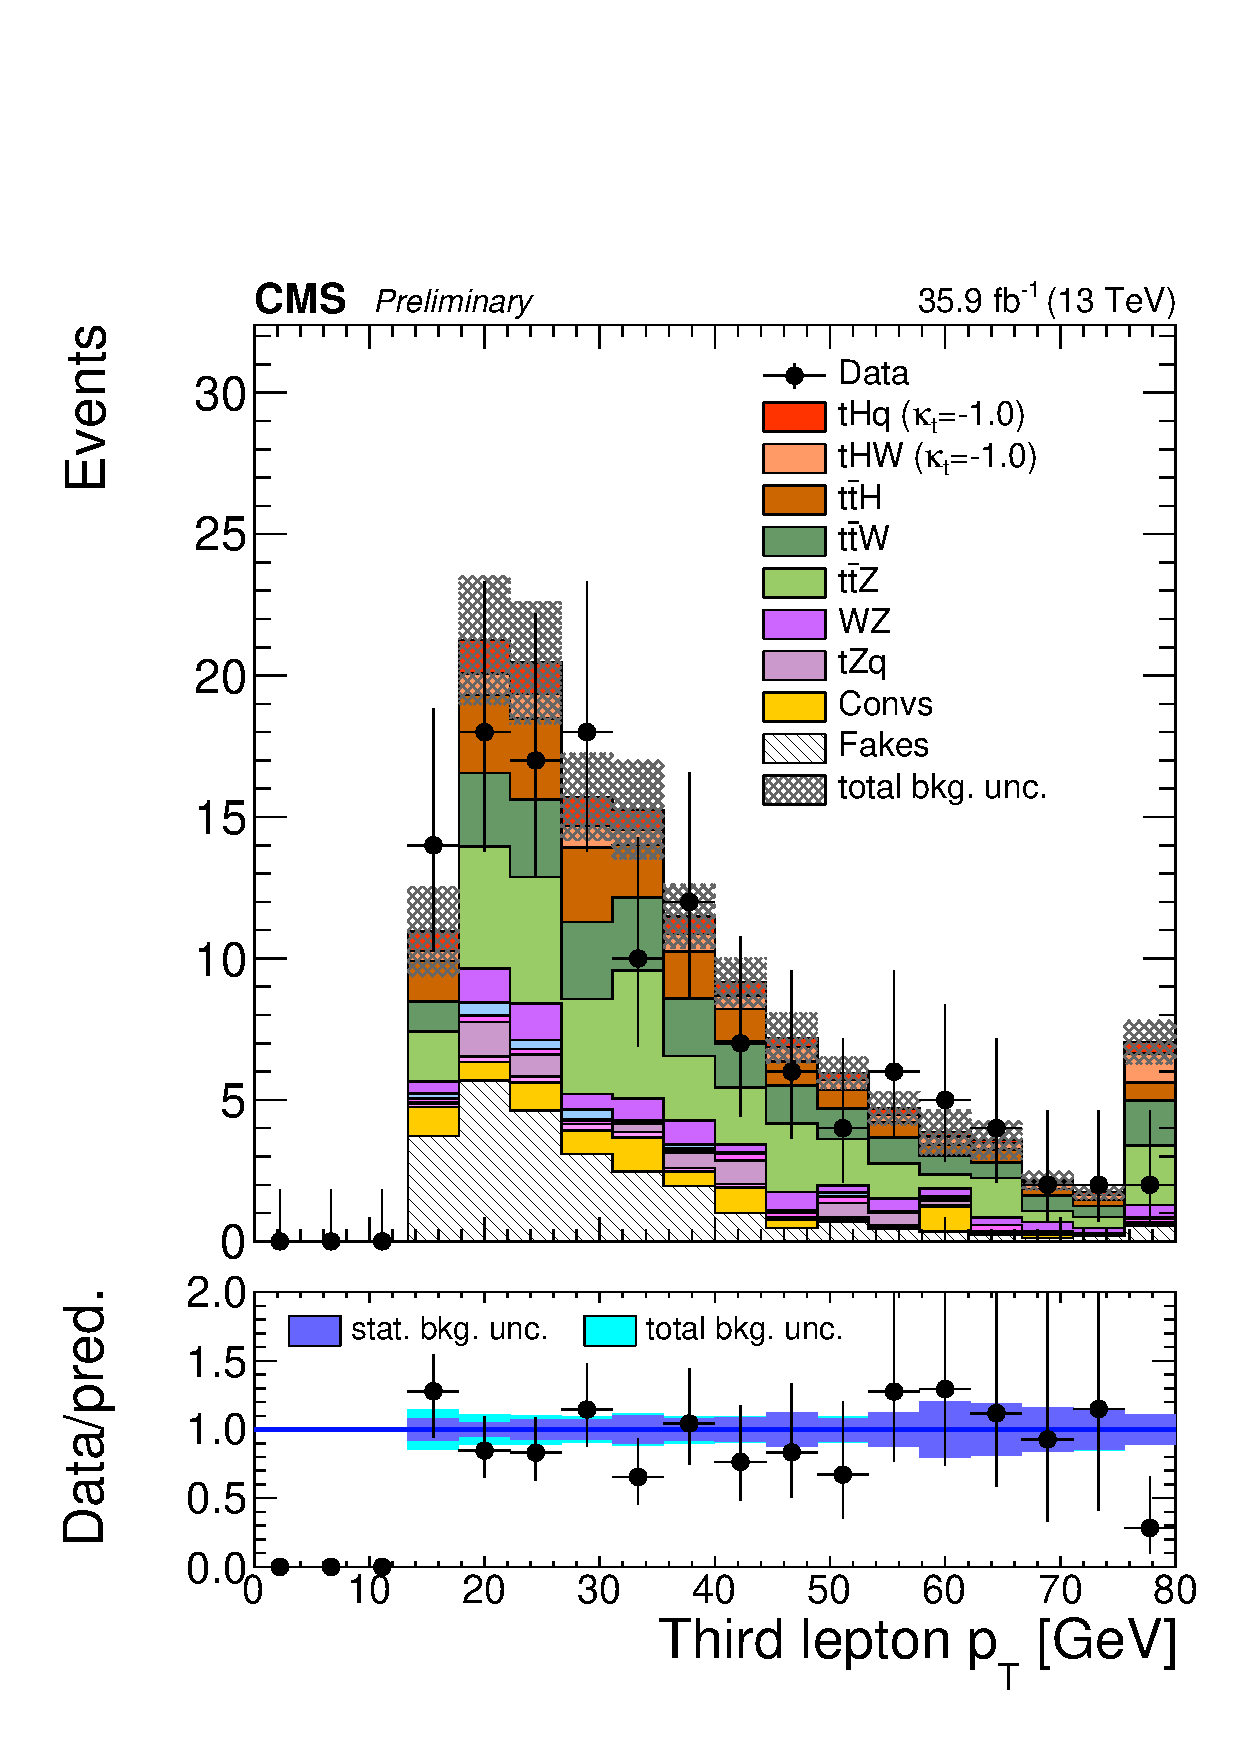
\includegraphics[width=0.22\textwidth]{figures/3lsignal/Lep3Pt.pdf} 
 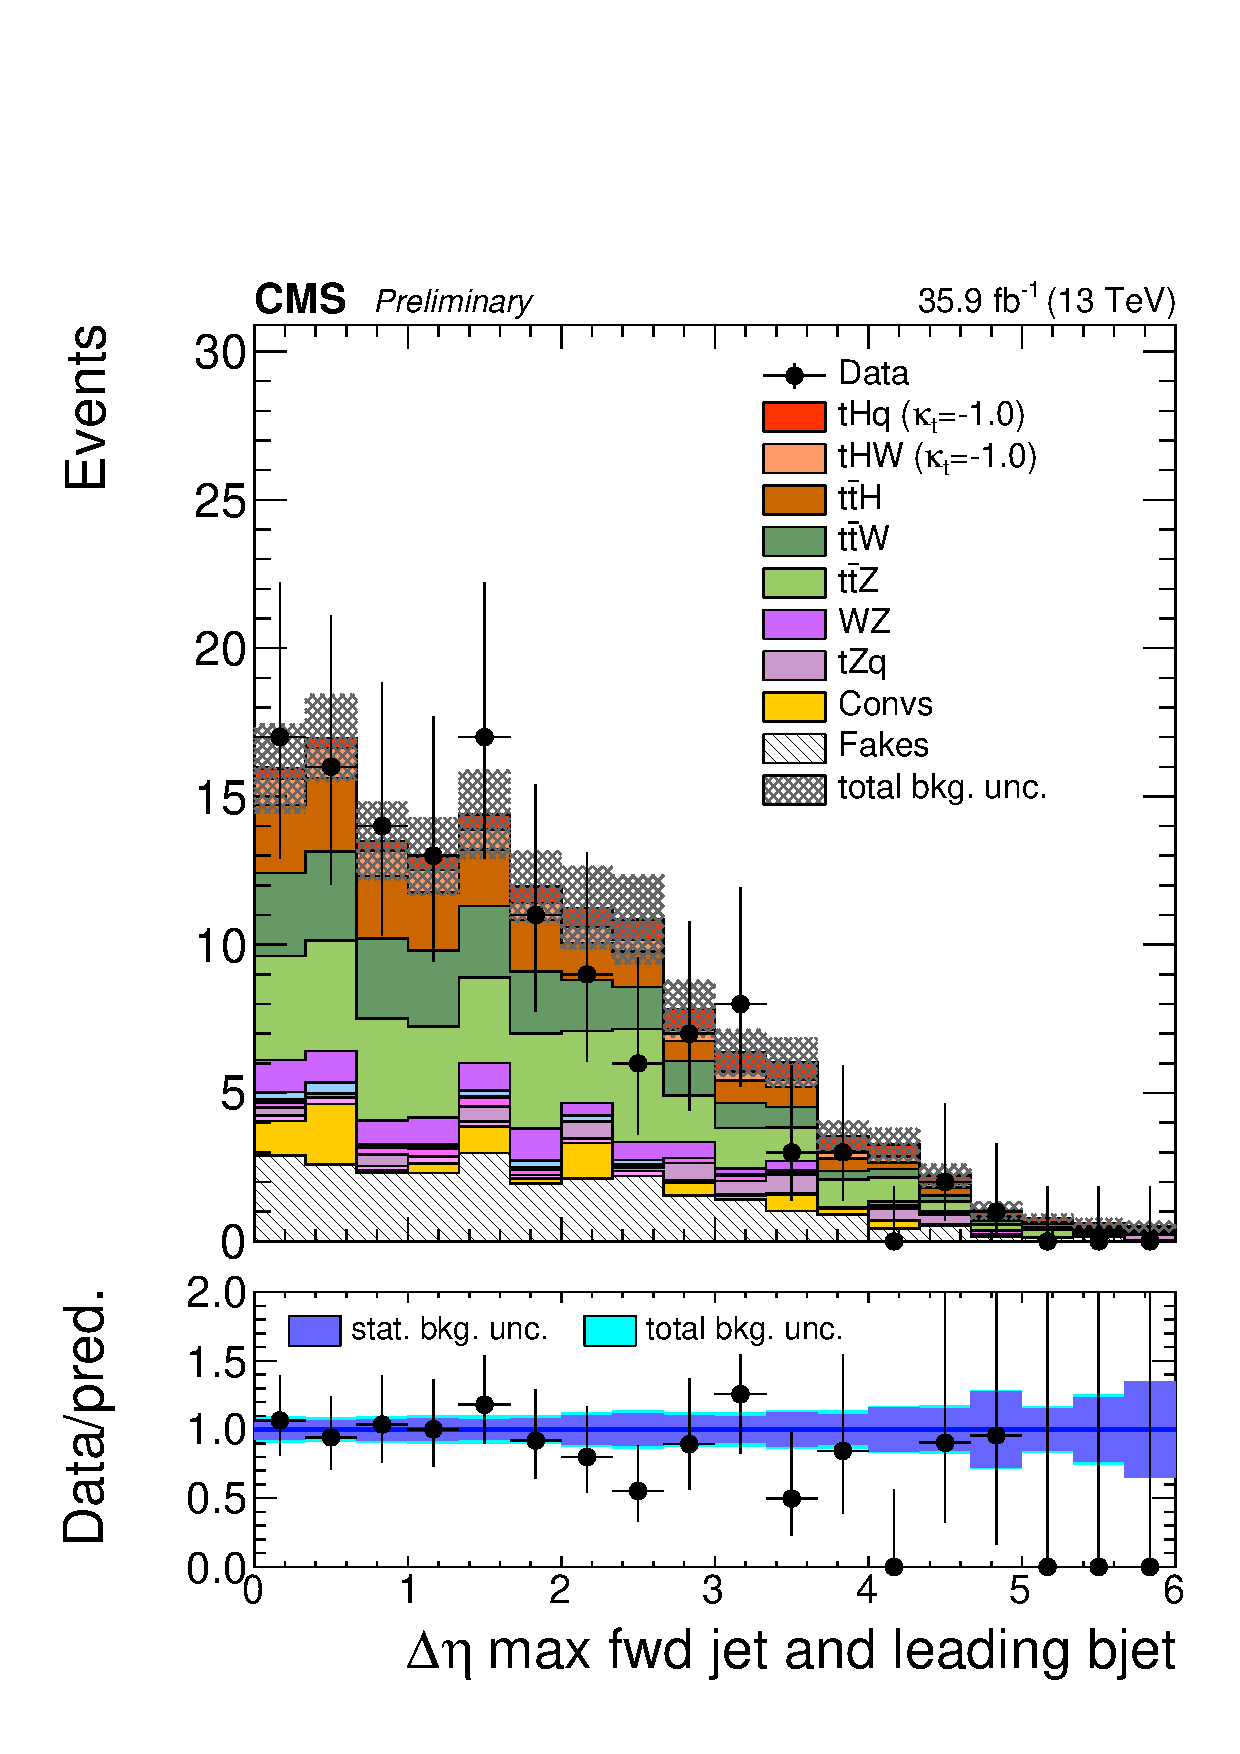
\includegraphics[width=0.22\textwidth]{figures/3lsignal/dEtaFwdJetBJet_40.pdf}
 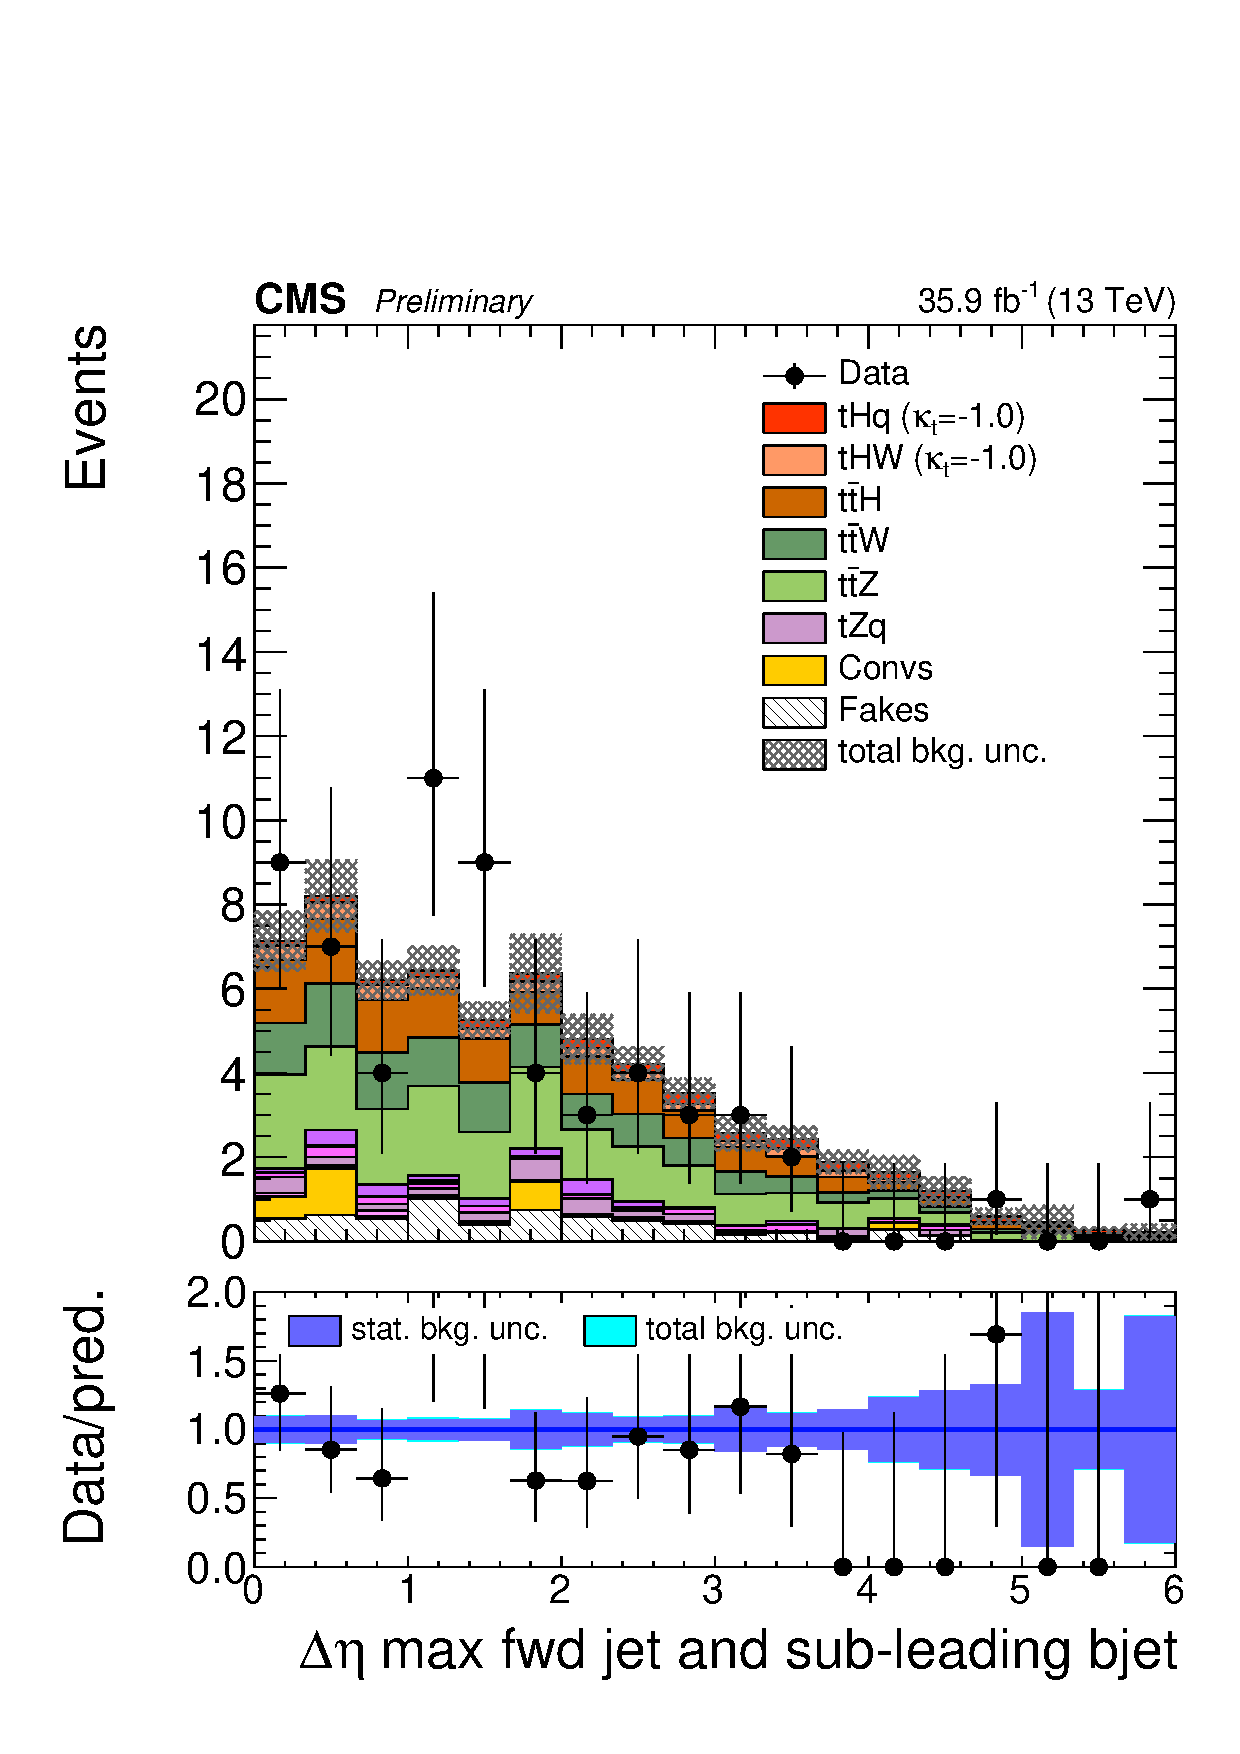
\includegraphics[width=0.22\textwidth]{figures/3lsignal/dEtaFwdJet2BJet_40.pdf}
 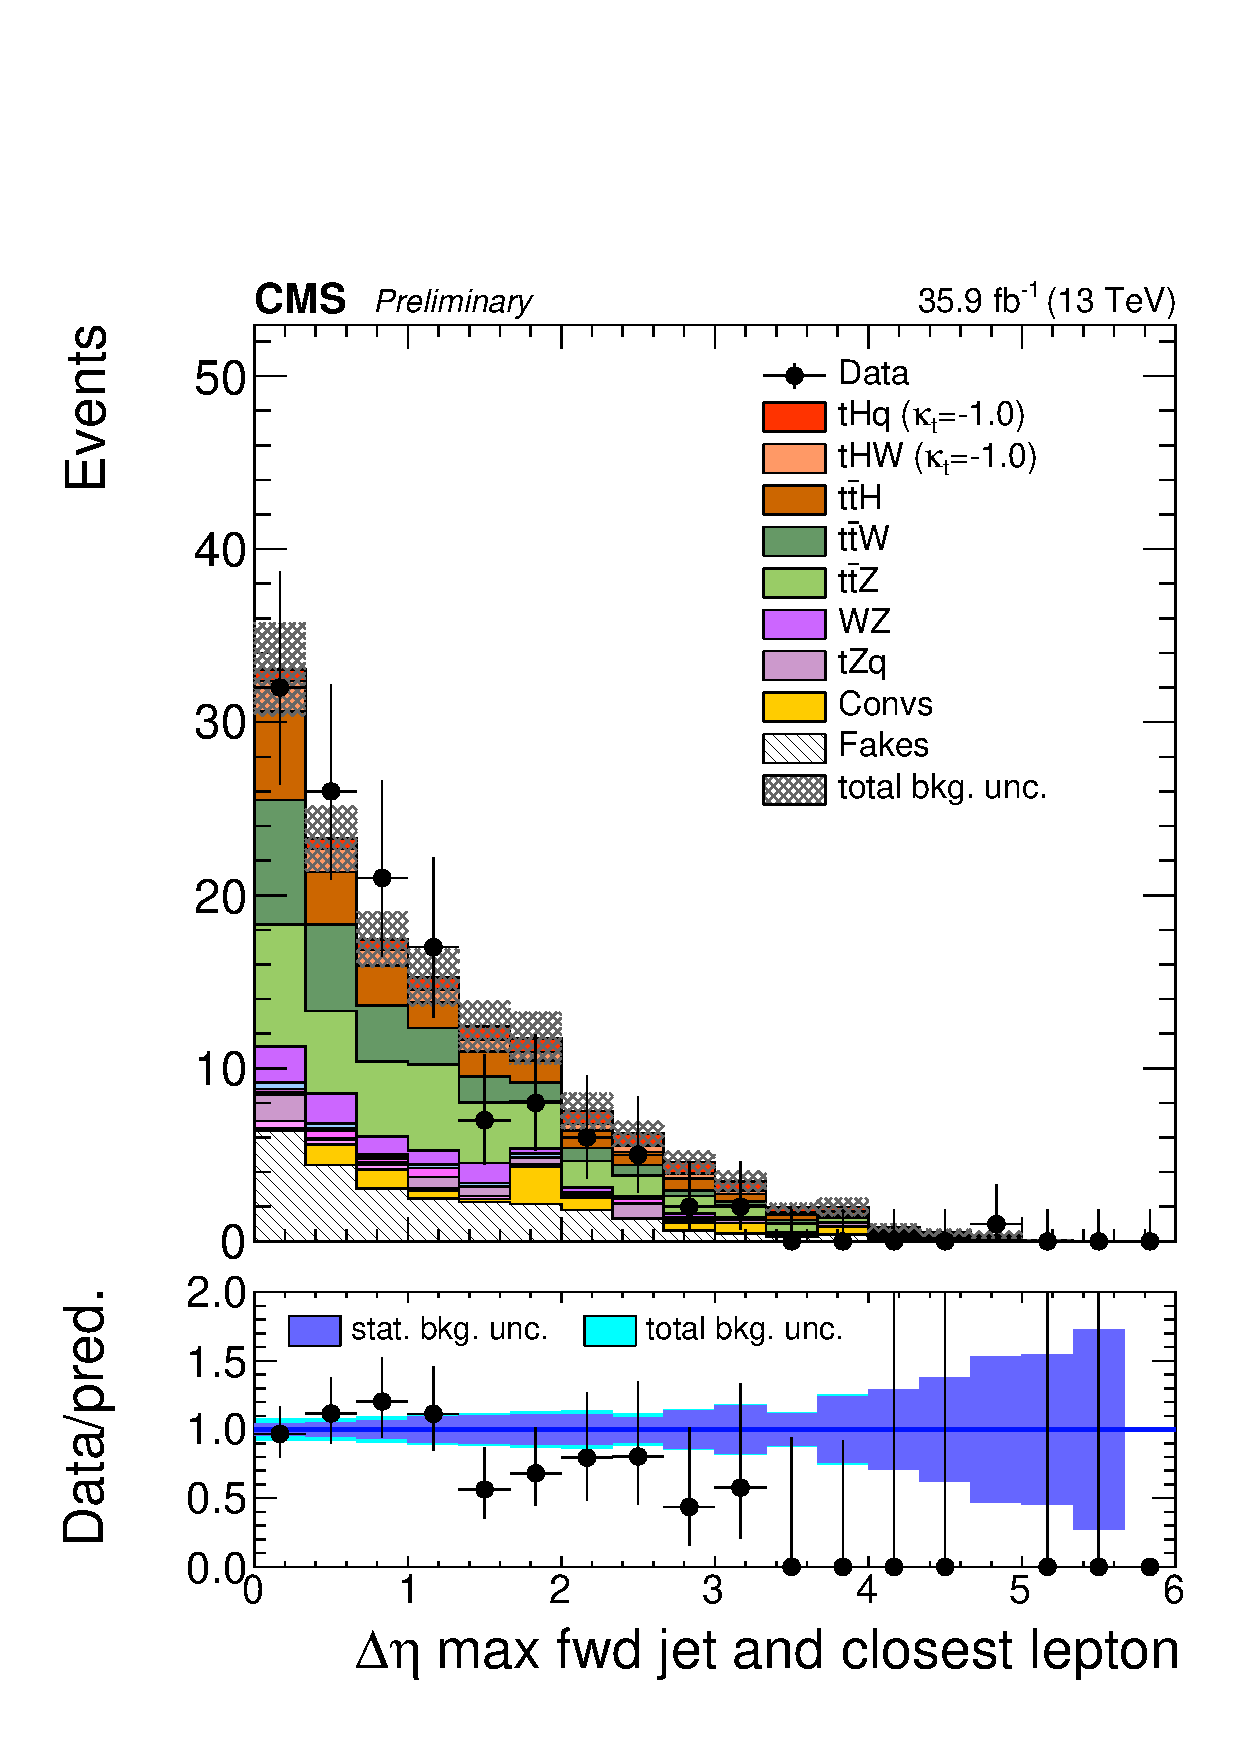
\includegraphics[width=0.22\textwidth]{figures/3lsignal/dEtaFwdJetClosestLep_40.pdf} \\
 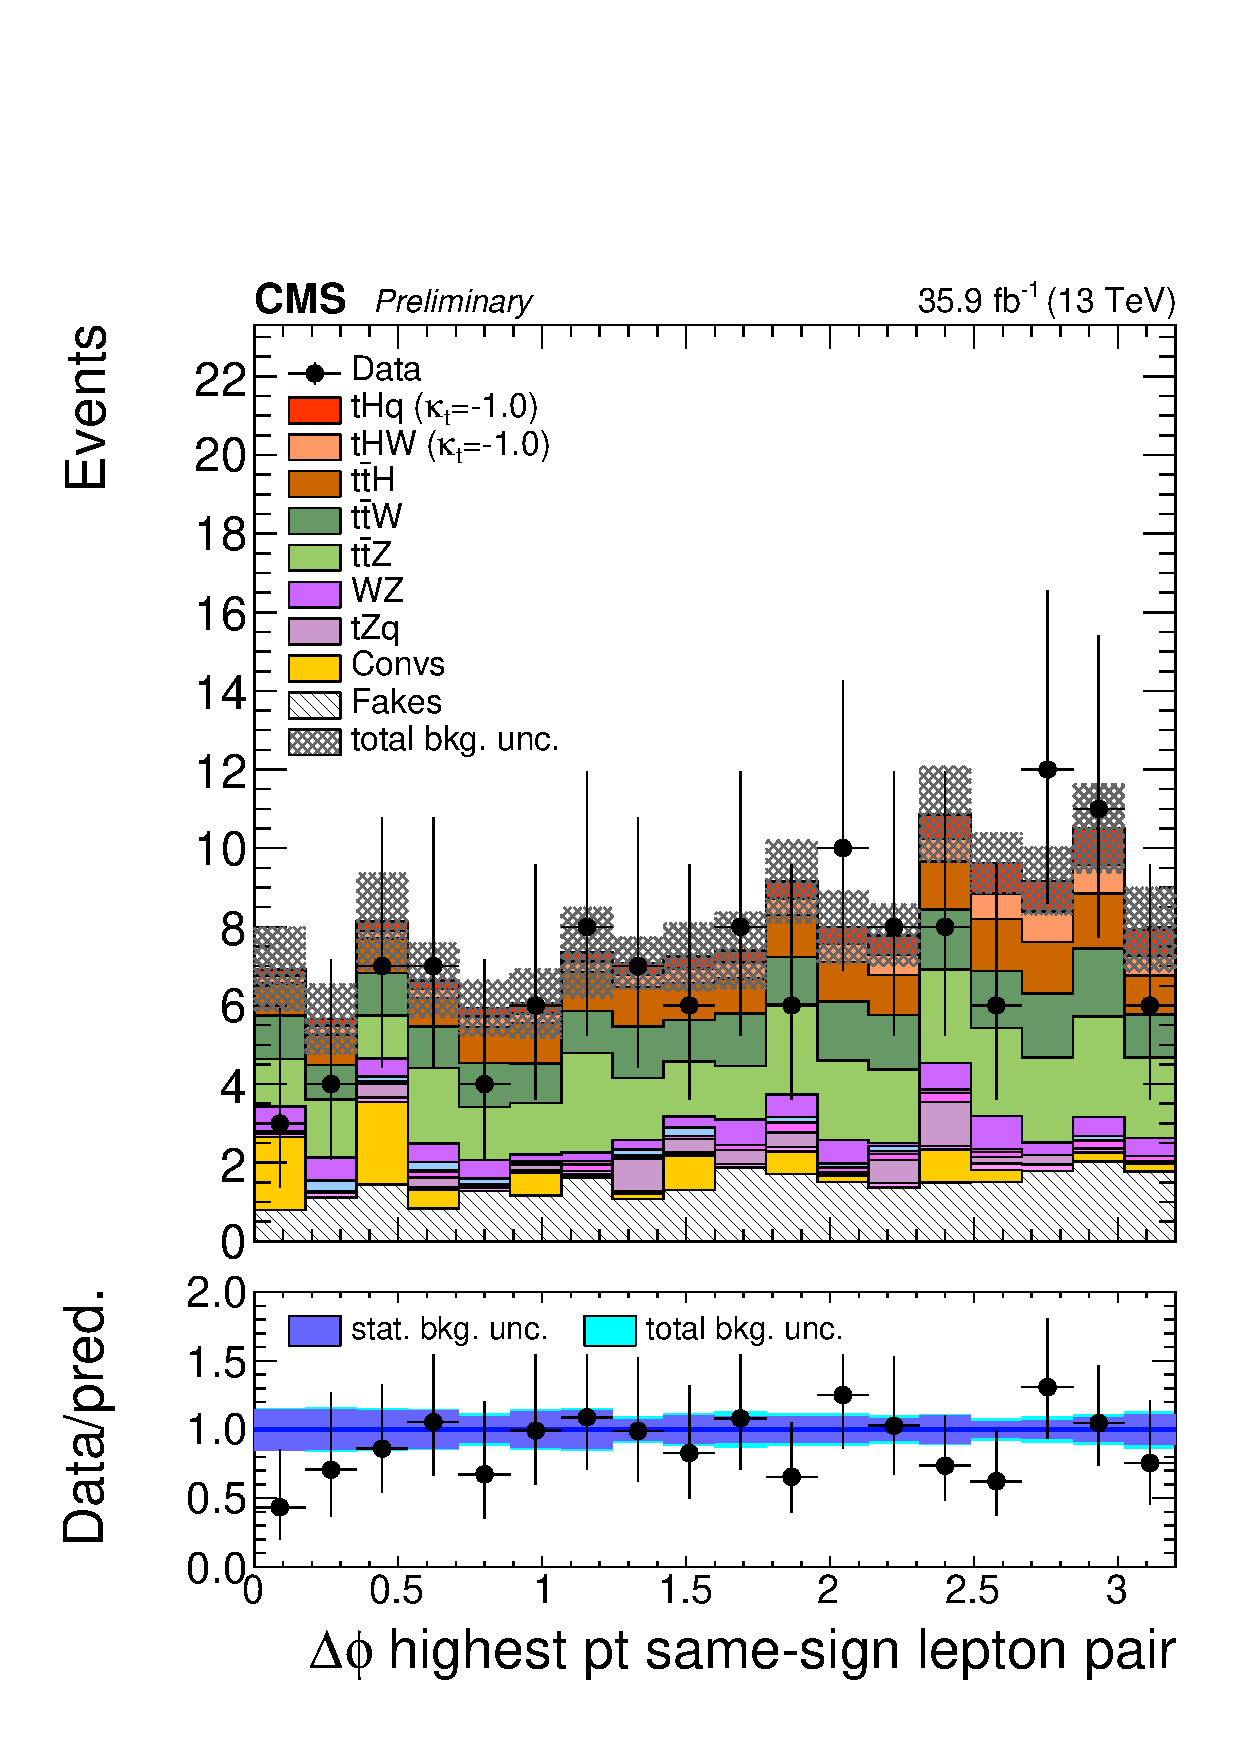
\includegraphics[width=0.22\textwidth]{figures/3lsignal/dPhiHighestPtSSPair.pdf}
 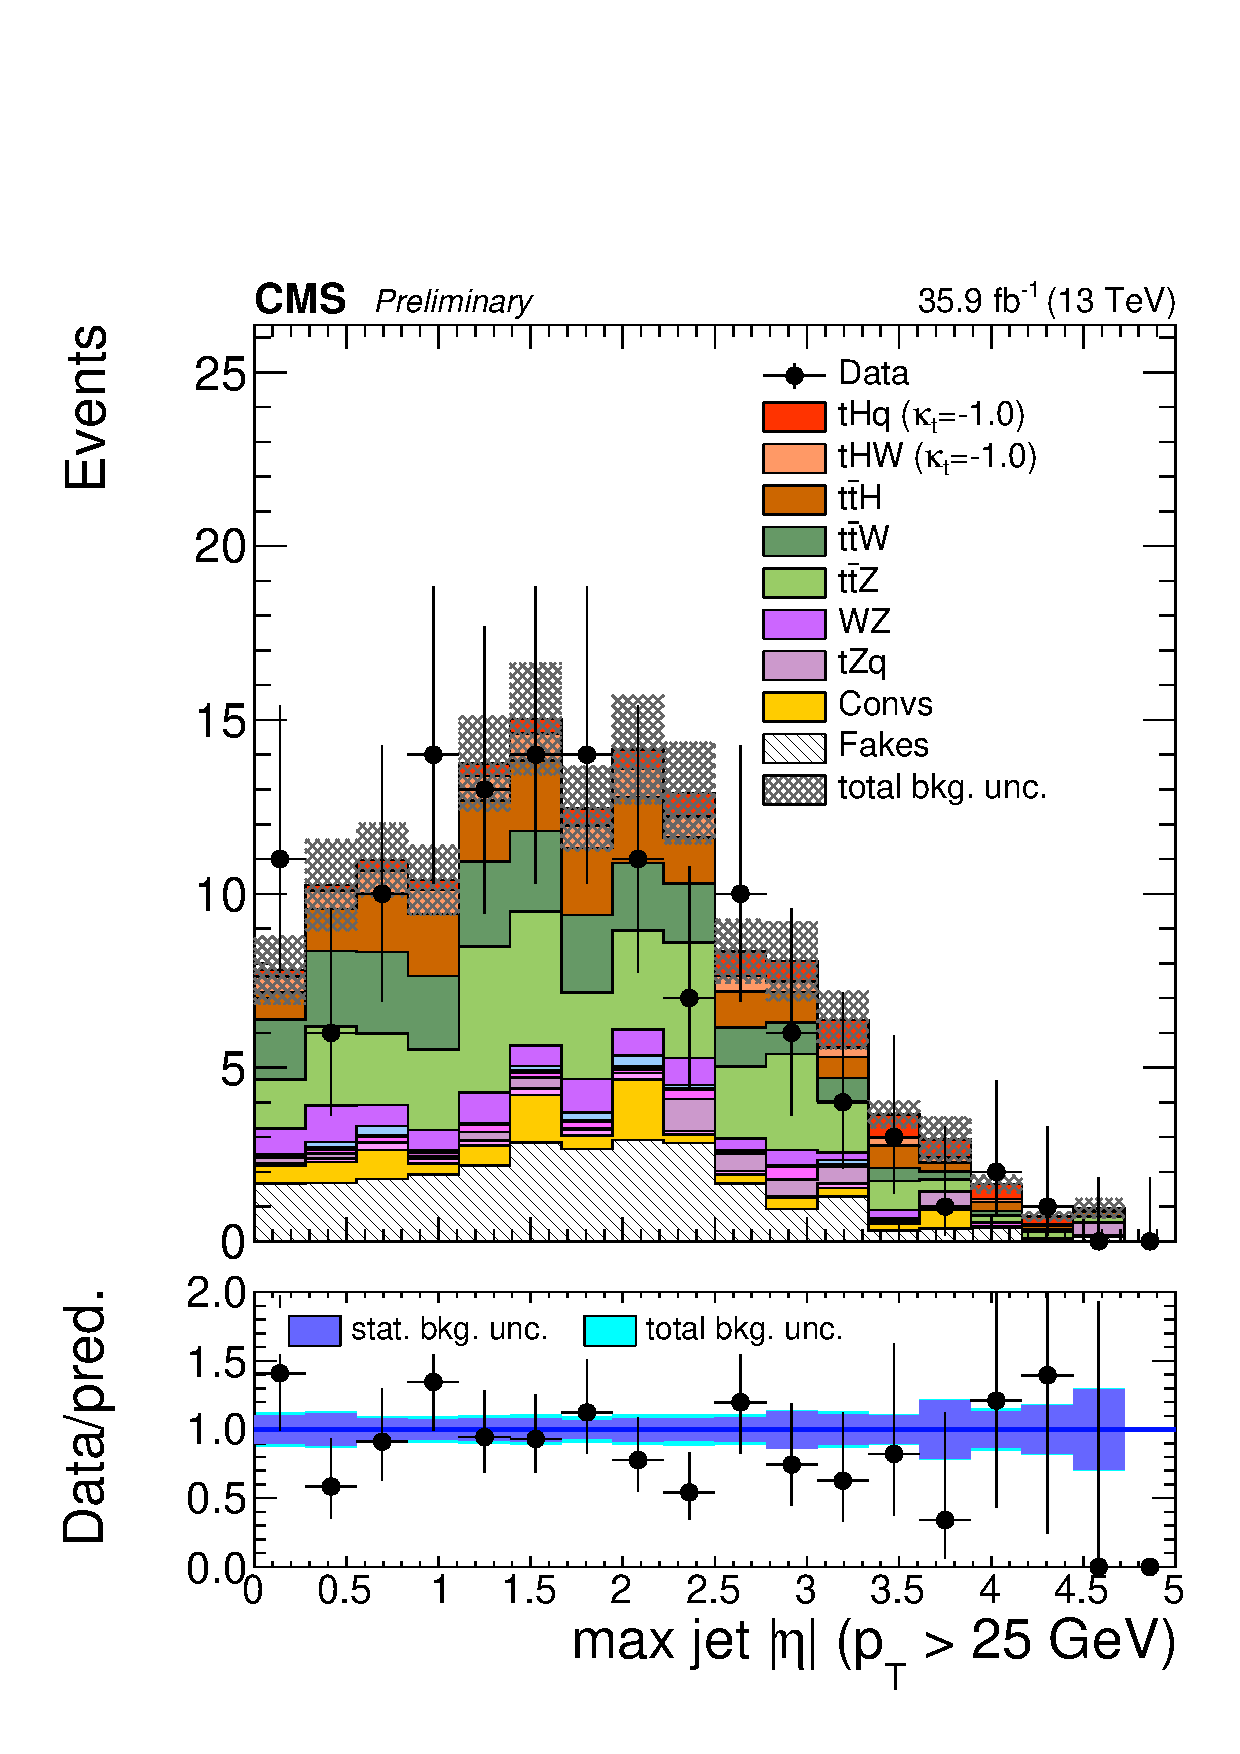
\includegraphics[width=0.22\textwidth]{figures/3lsignal/maxEtaJet25_40.pdf}
 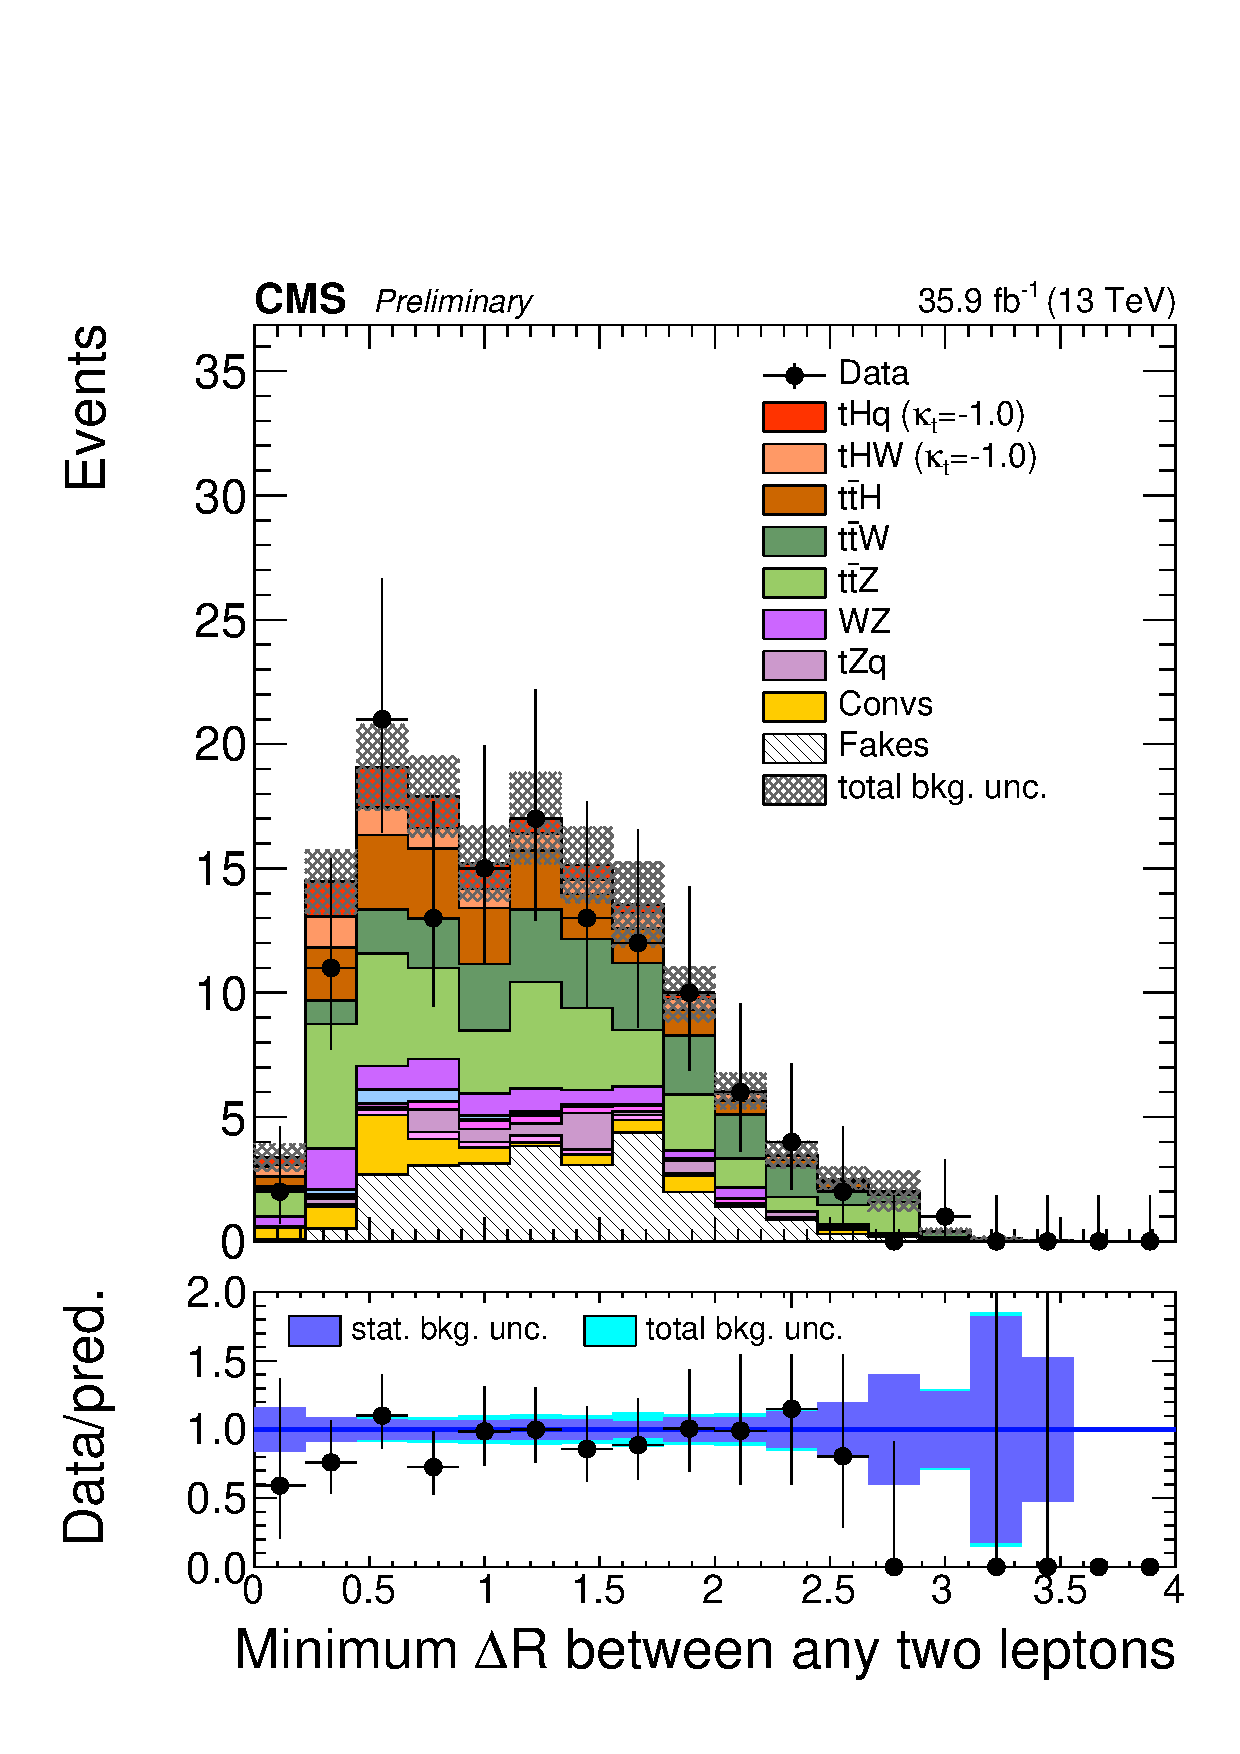
\includegraphics[width=0.22\textwidth]{figures/3lsignal/minDRll.pdf}
 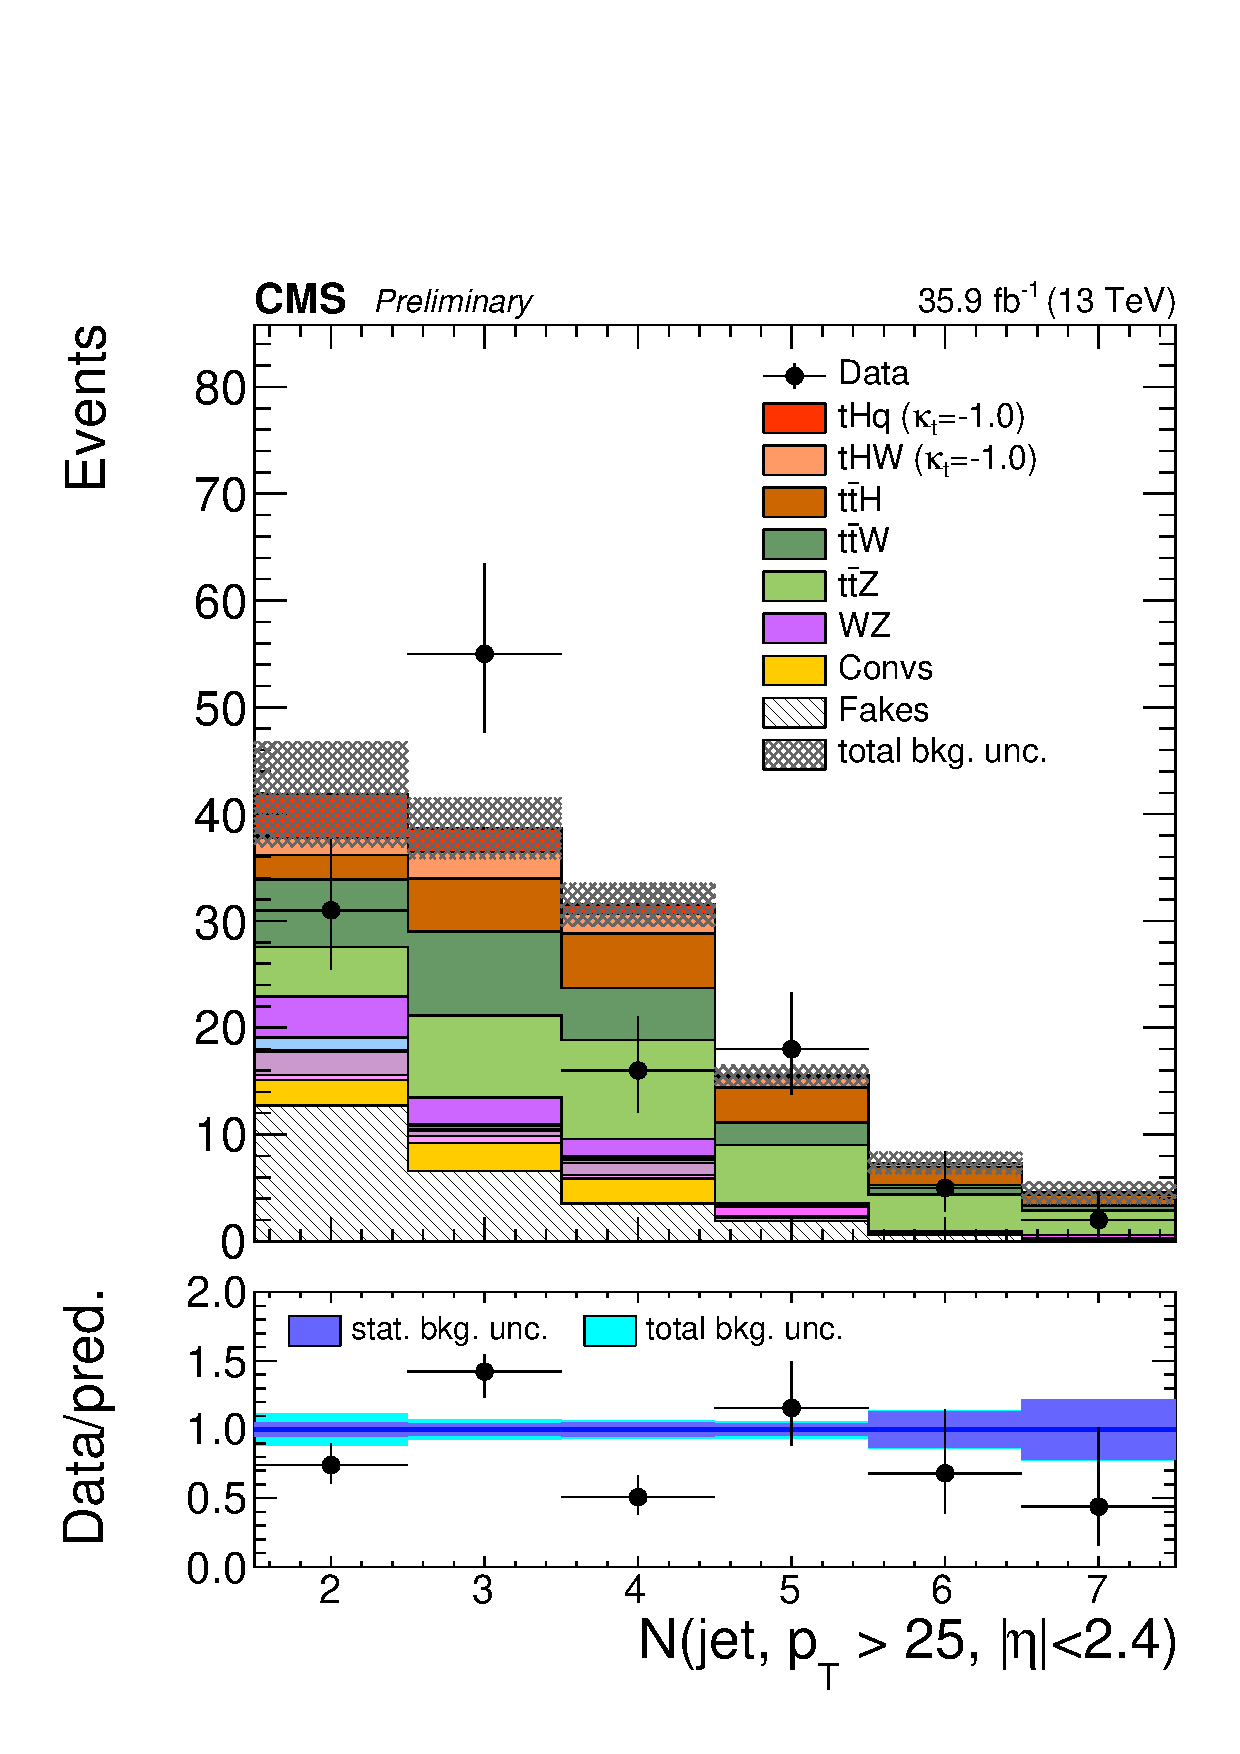
\includegraphics[width=0.22\textwidth]{figures/3lsignal/nJet25.pdf} \\
 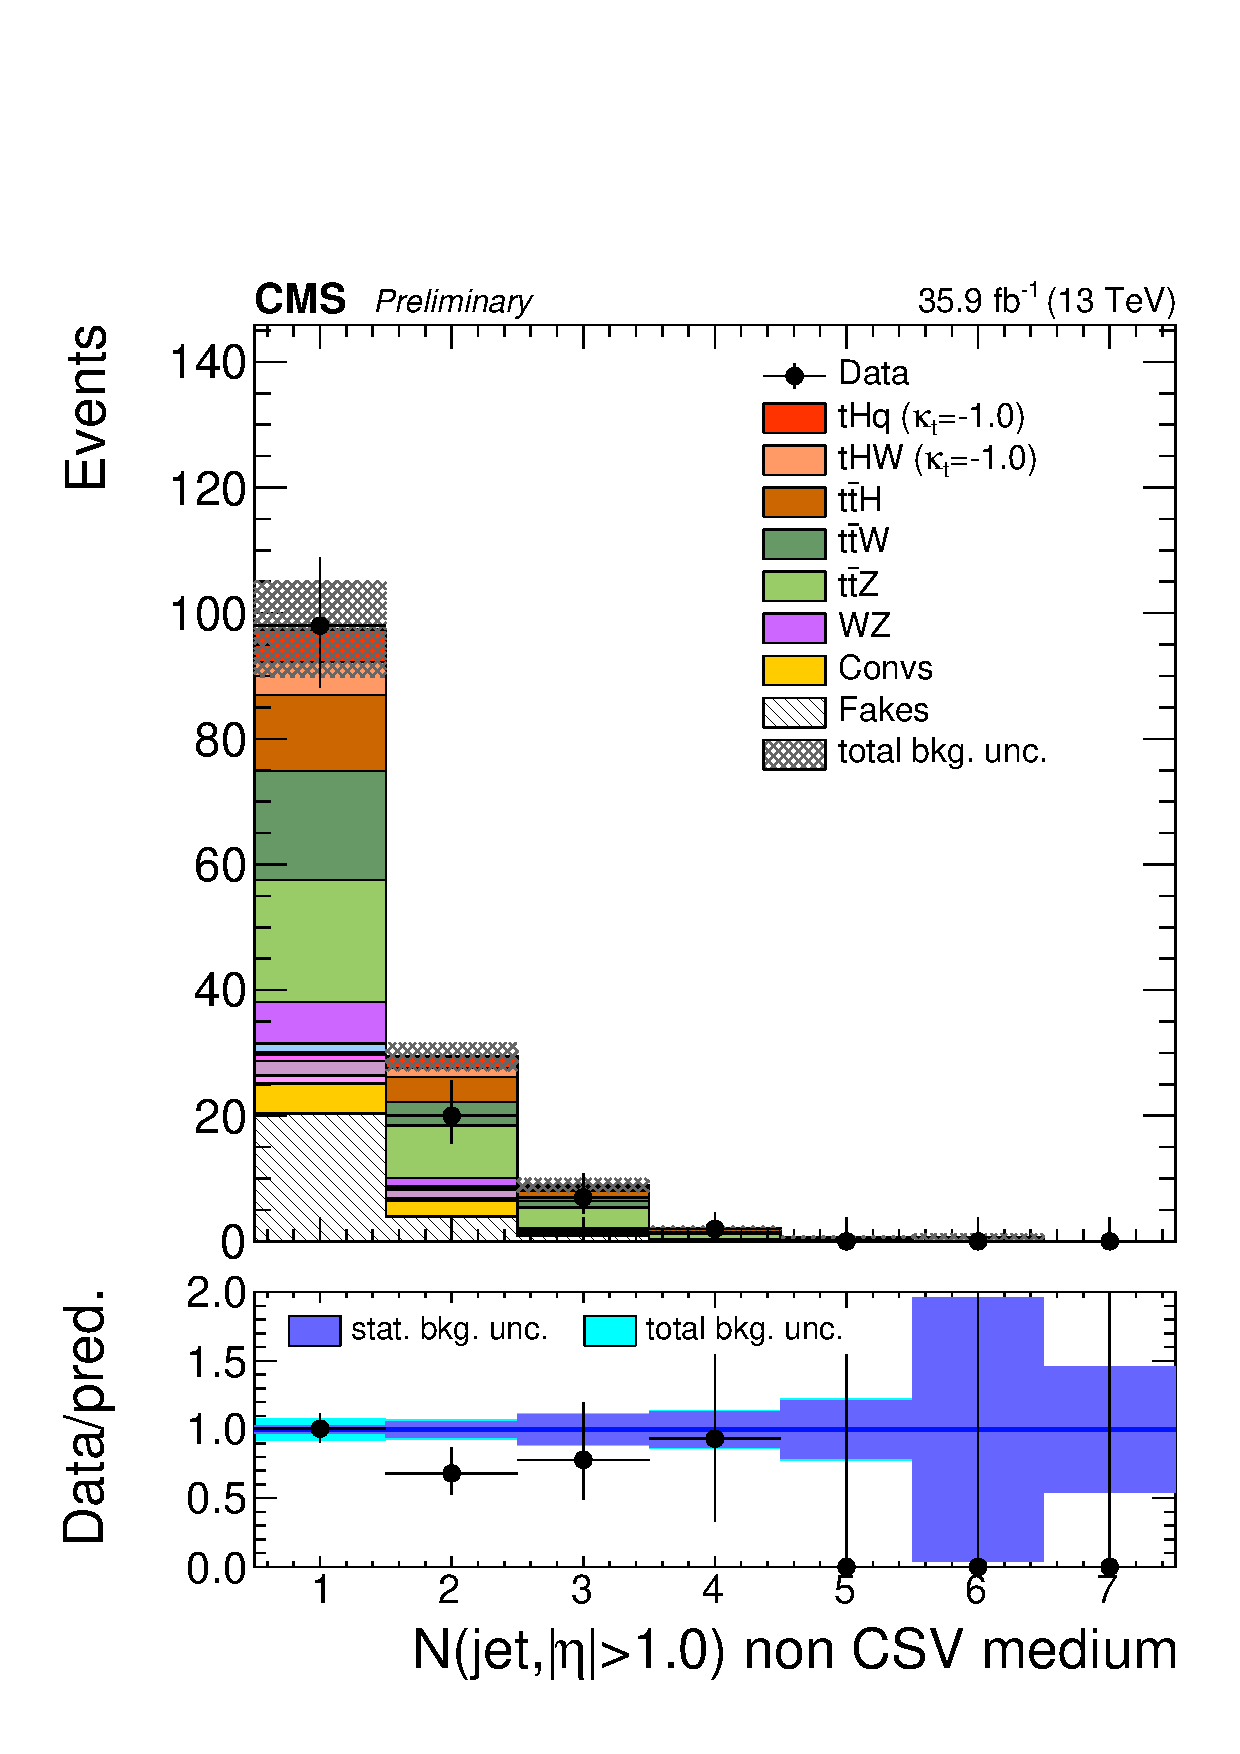
\includegraphics[width=0.22\textwidth]{figures/3lsignal/nJetEta1_40.pdf}
 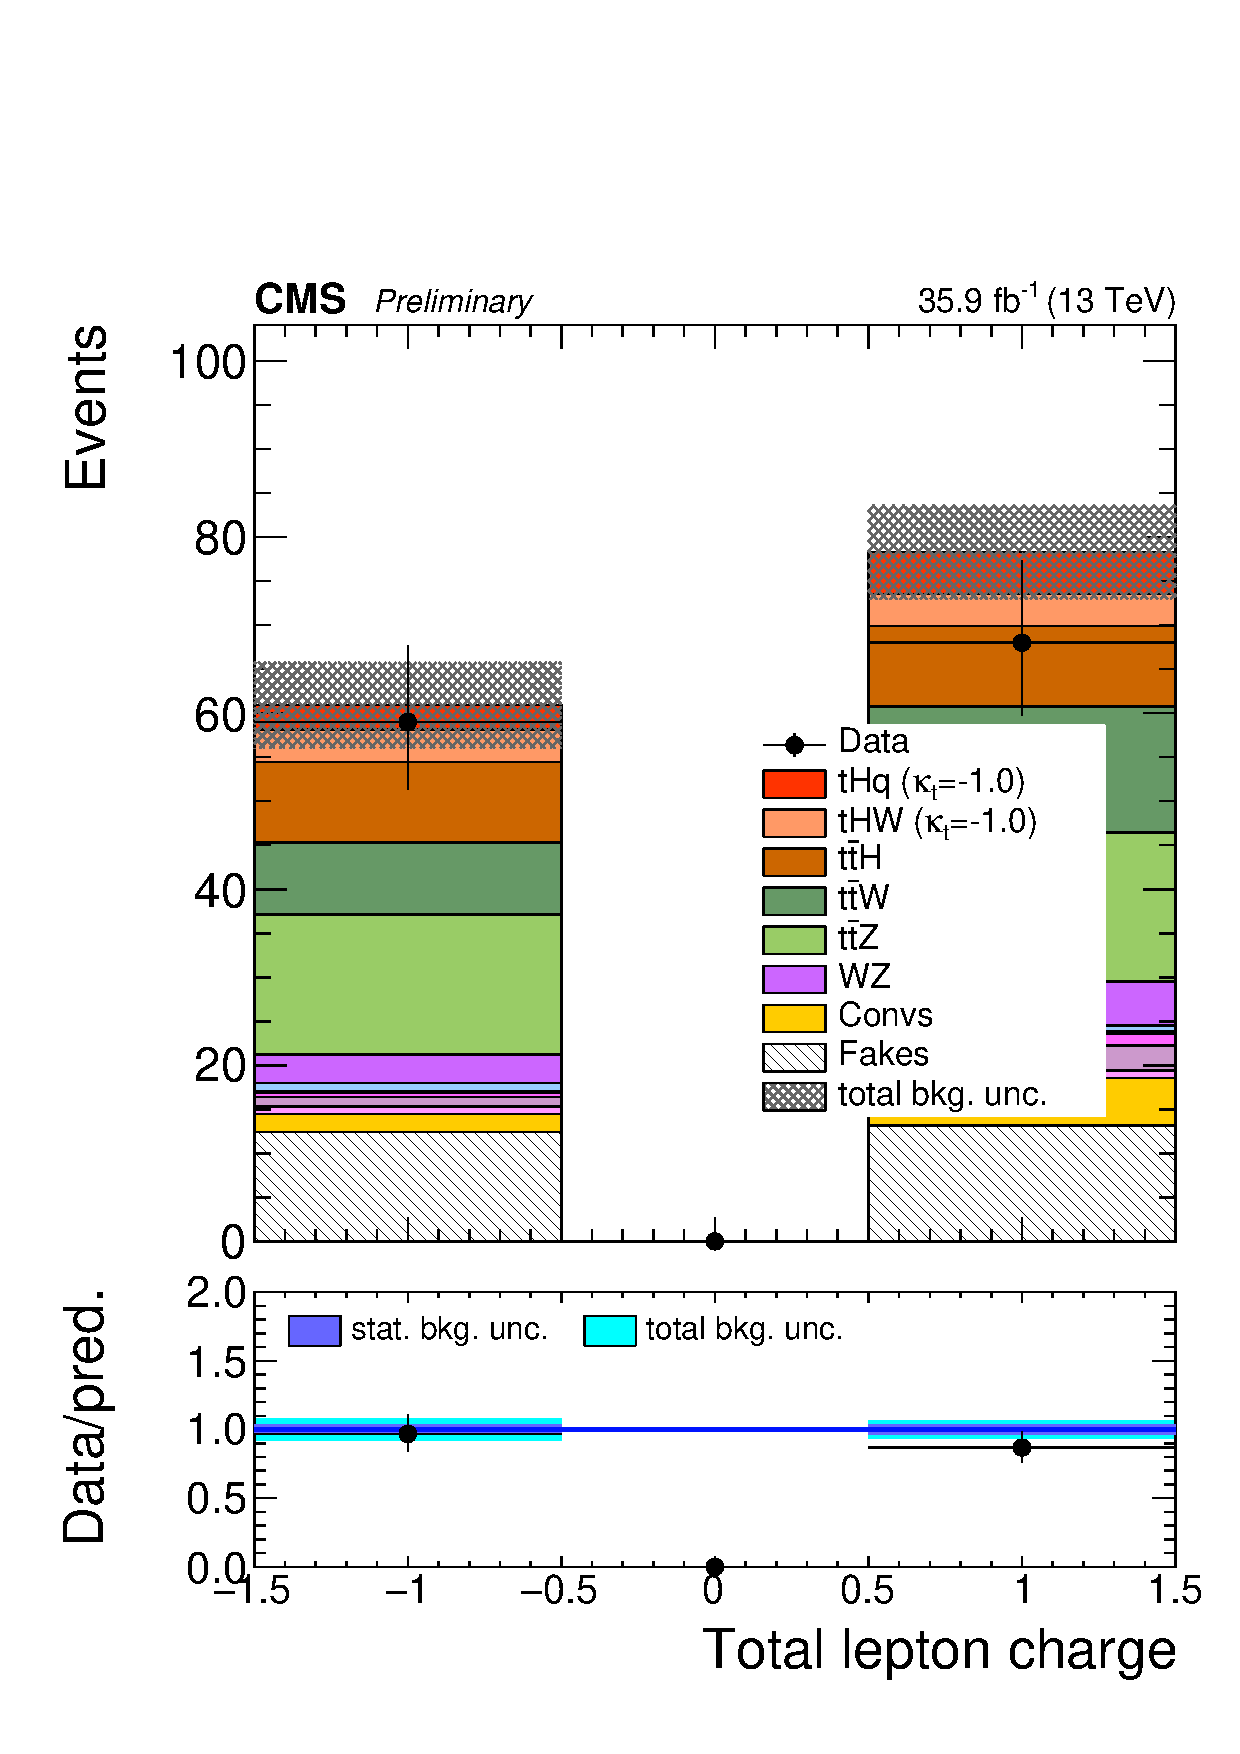
\includegraphics[width=0.22\textwidth]{figures/3lsignal/totCharge.pdf}
\caption{Distributions of input variables to the BDT for signal discrimination, three lepton channel, normalized to their cross section and to 35.9\fbinv.} 
\label{fig:input_vars_3l_xsec}
\end{figure}    

\begin{figure} [!h]
  \centering
  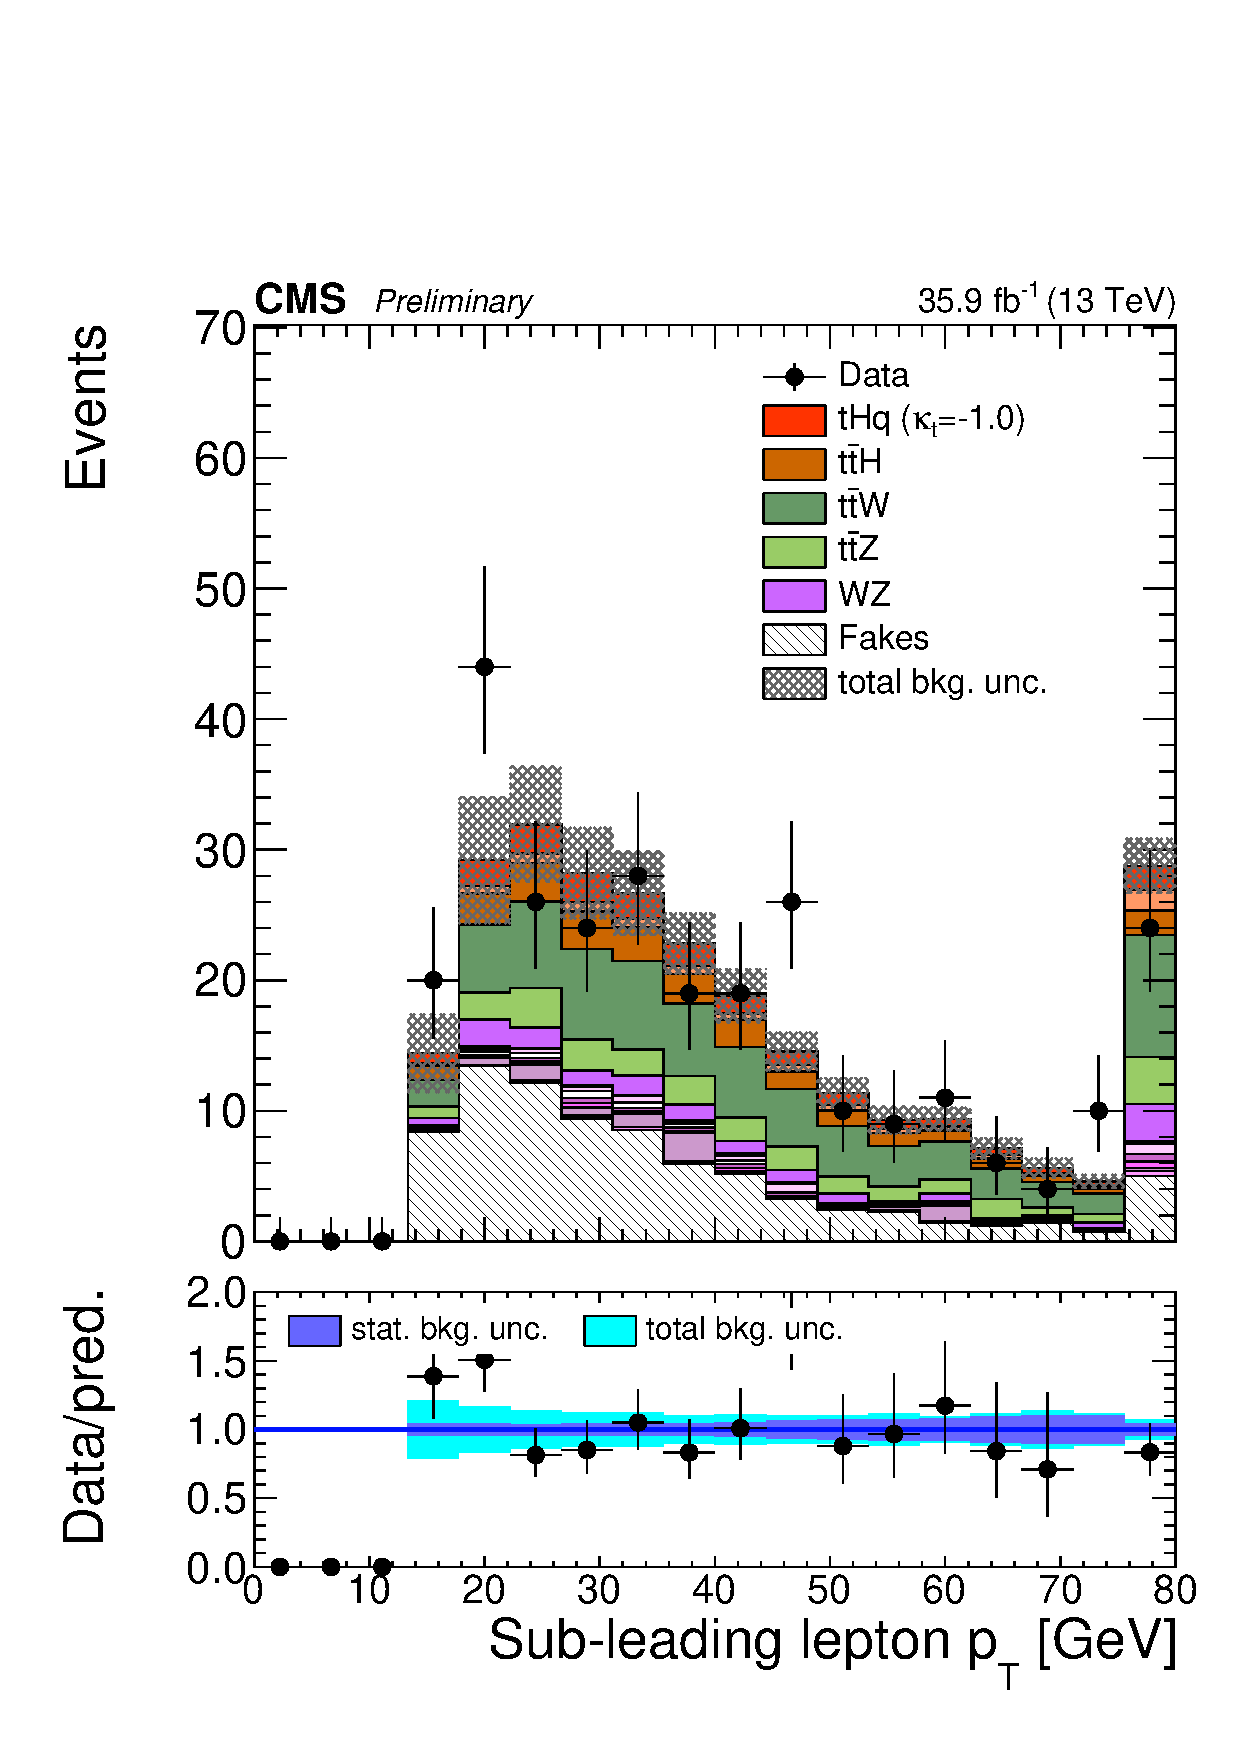
\includegraphics[width=0.22\textwidth]{figures/signalregion_2lss/mumu/Lep2Pt.pdf}
  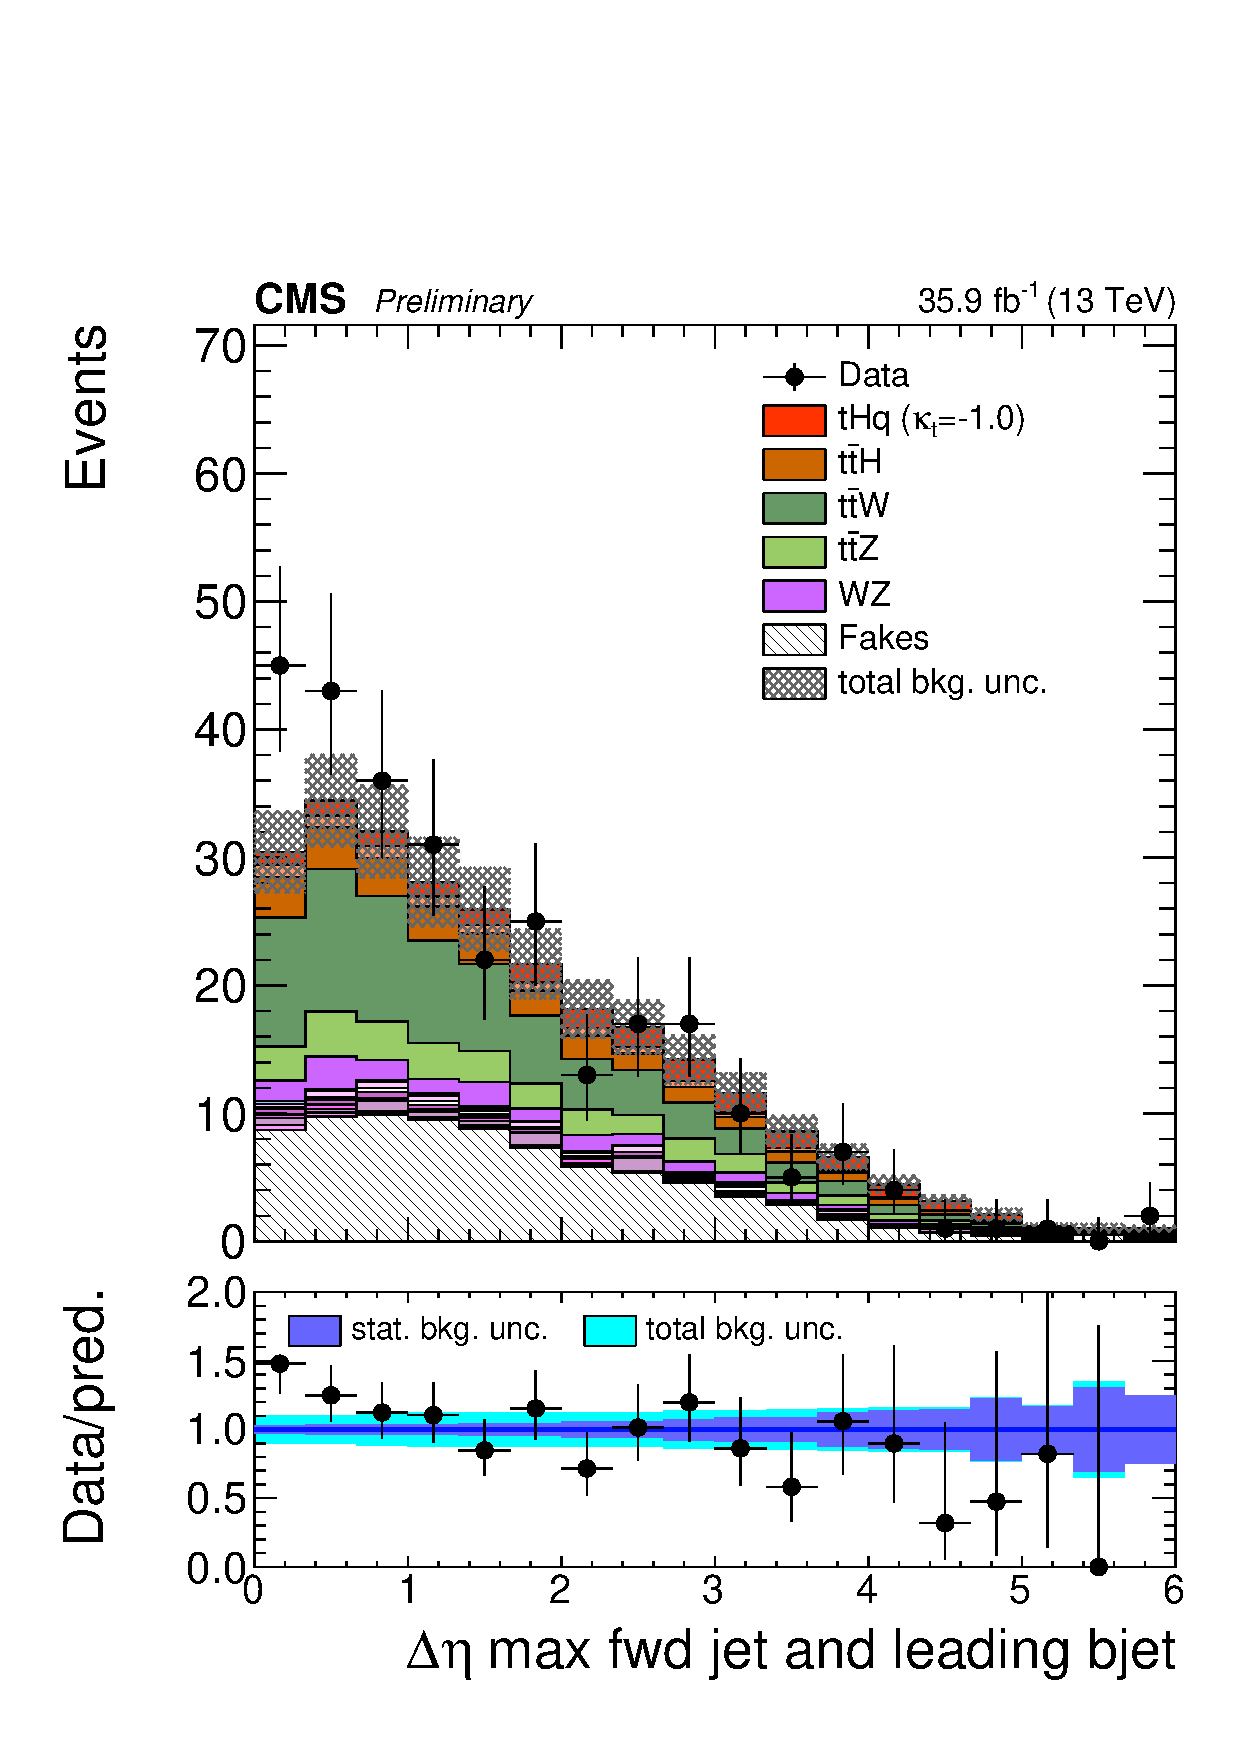
\includegraphics[width=0.22\textwidth]{figures/signalregion_2lss/mumu/dEtaFwdJetBJet_40.pdf}
  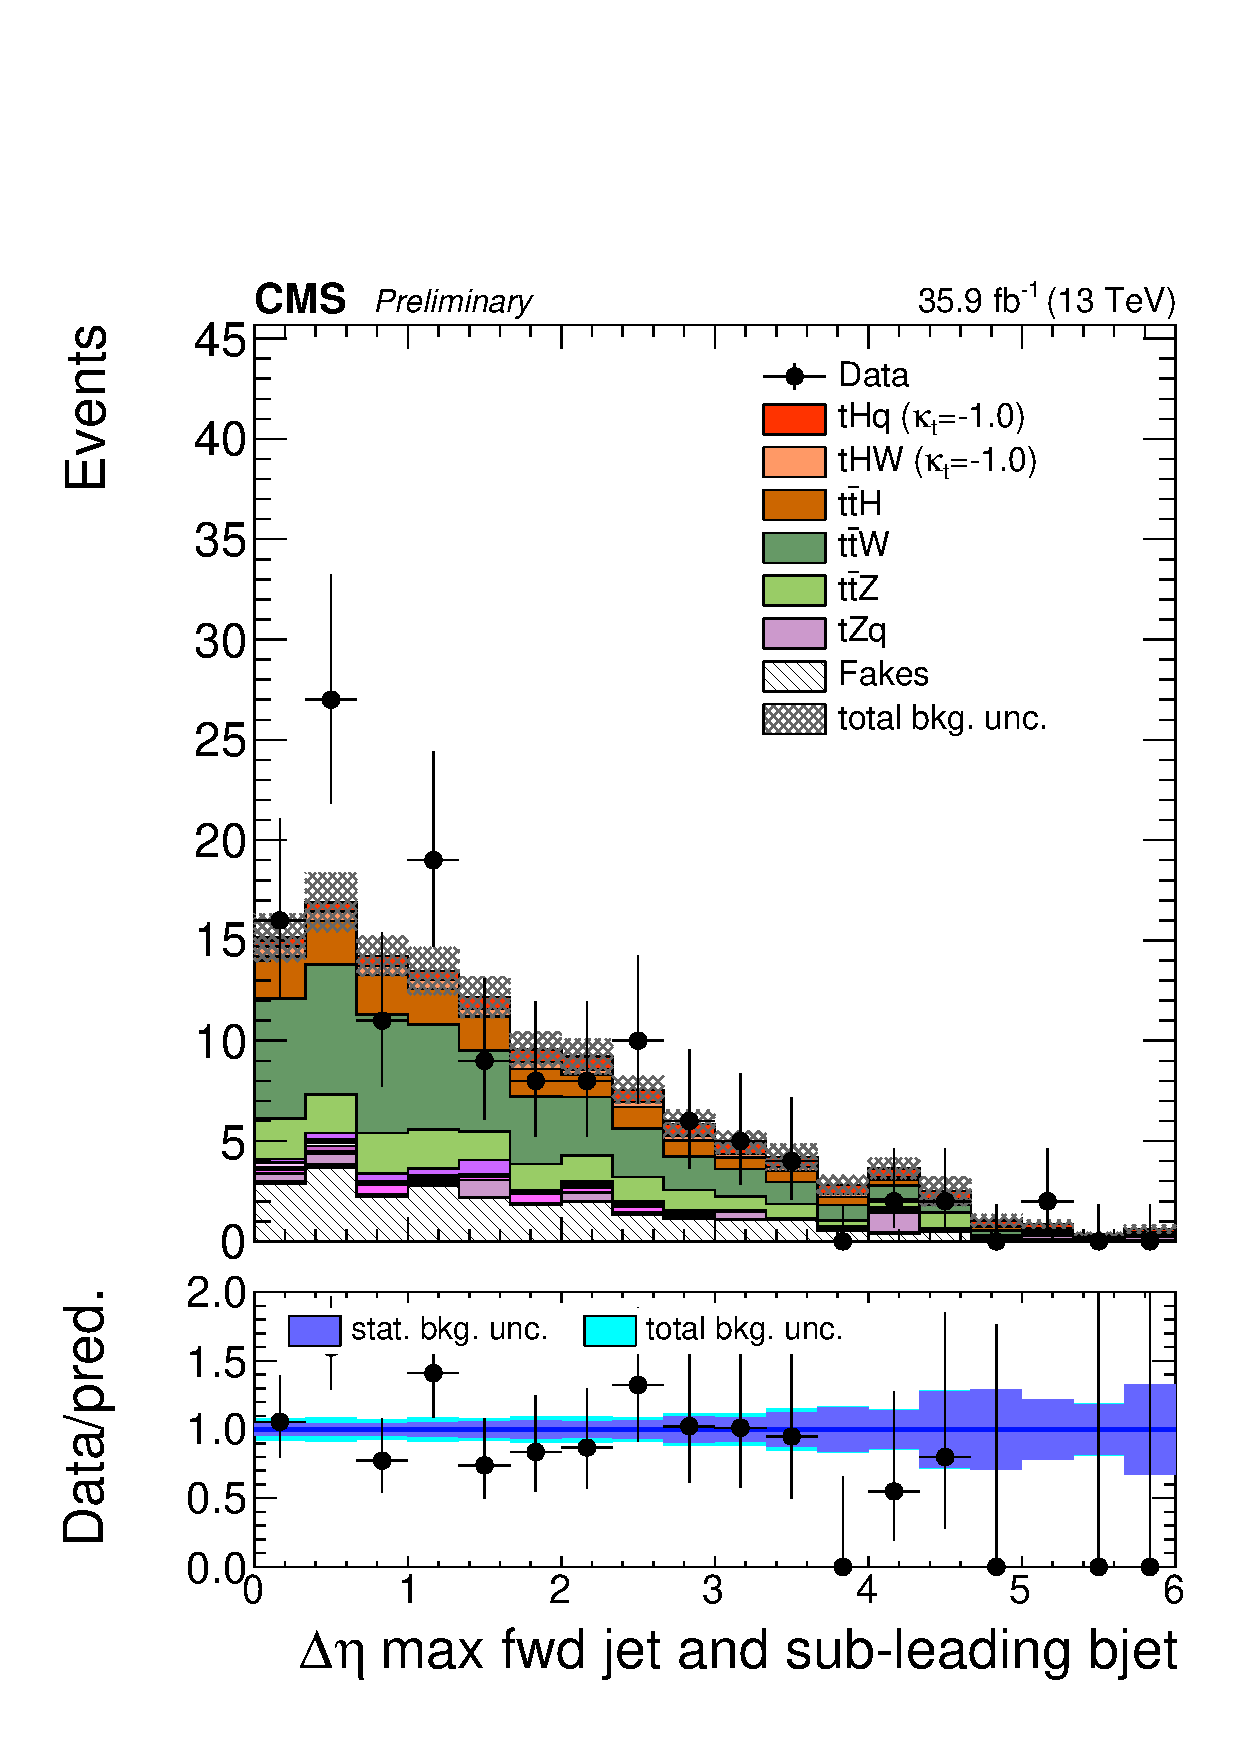
\includegraphics[width=0.22\textwidth]{figures/signalregion_2lss/mumu/dEtaFwdJet2BJet_40.pdf}
  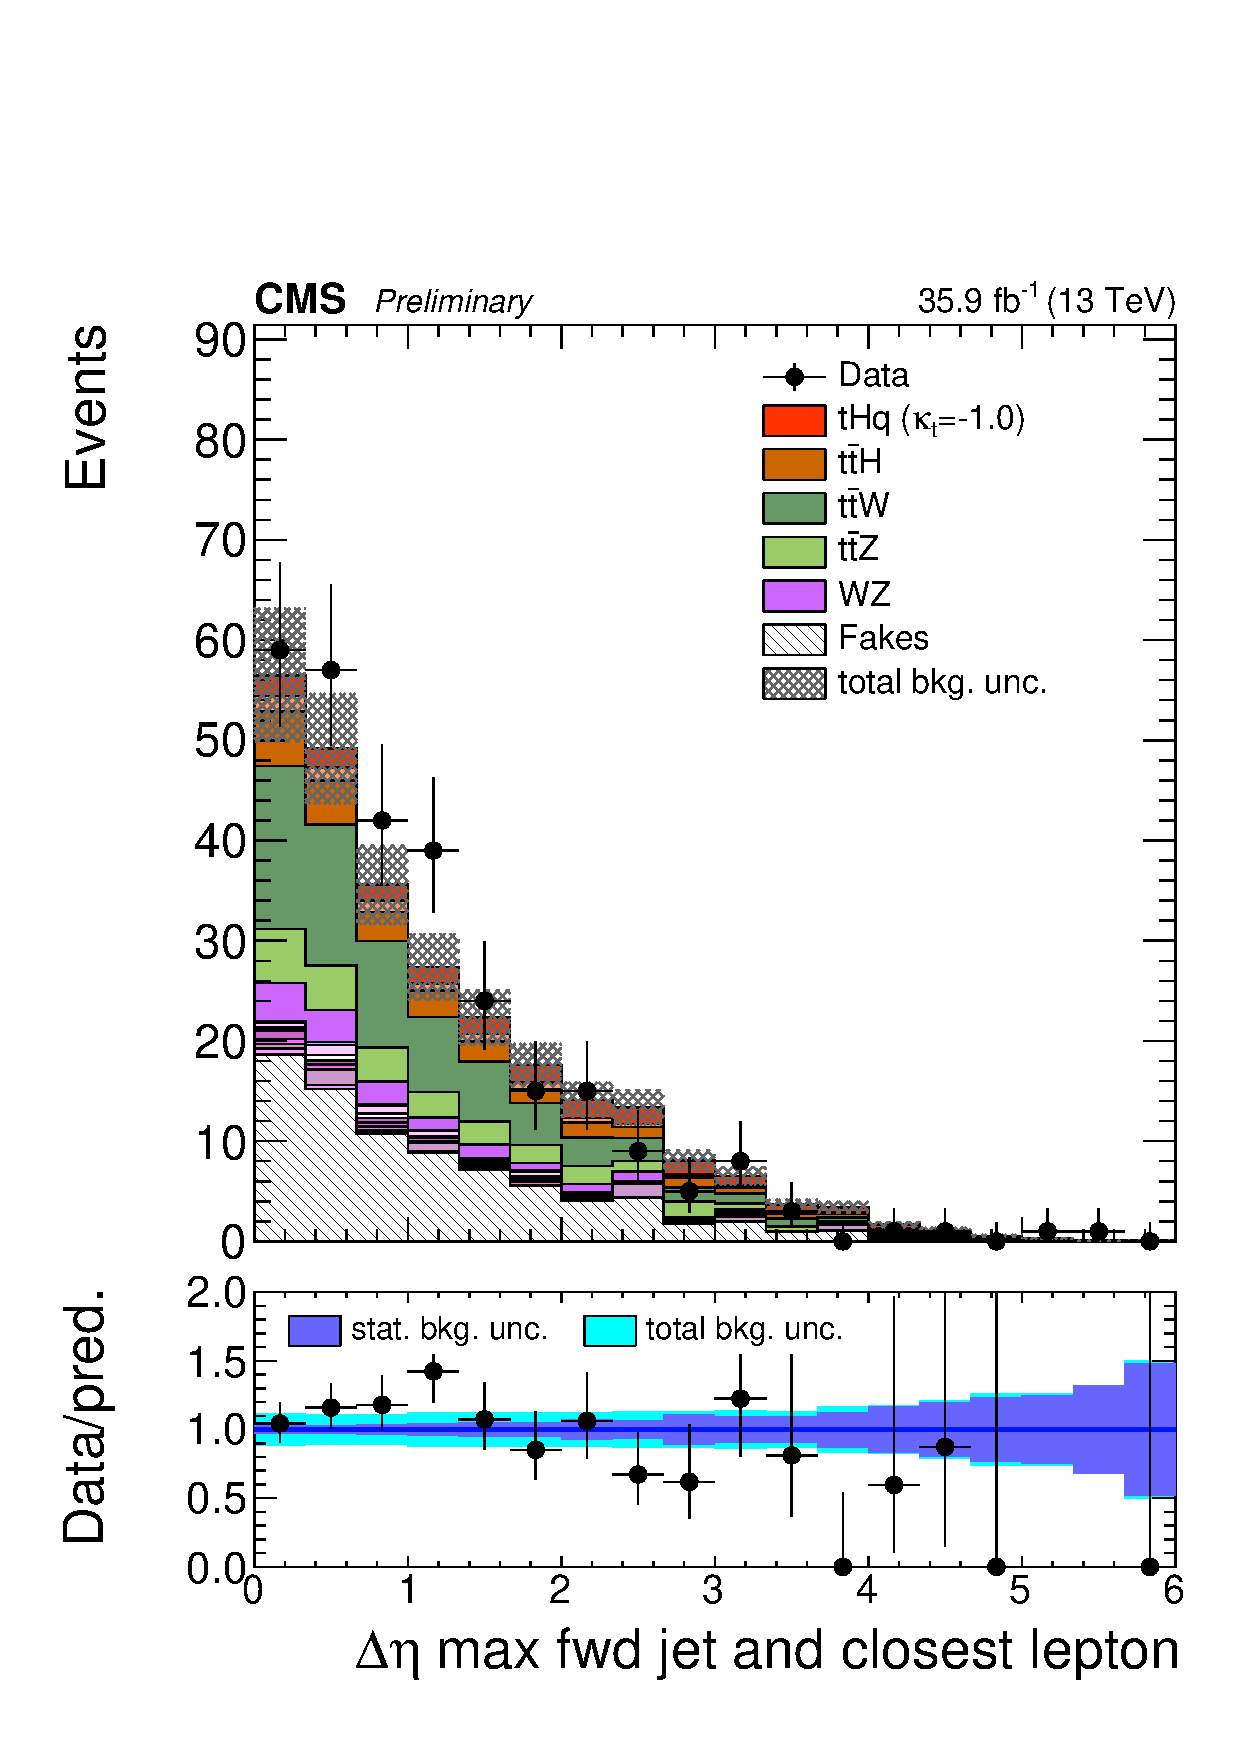
\includegraphics[width=0.22\textwidth]{figures/signalregion_2lss/mumu/dEtaFwdJetClosestLep_40.pdf} \\
  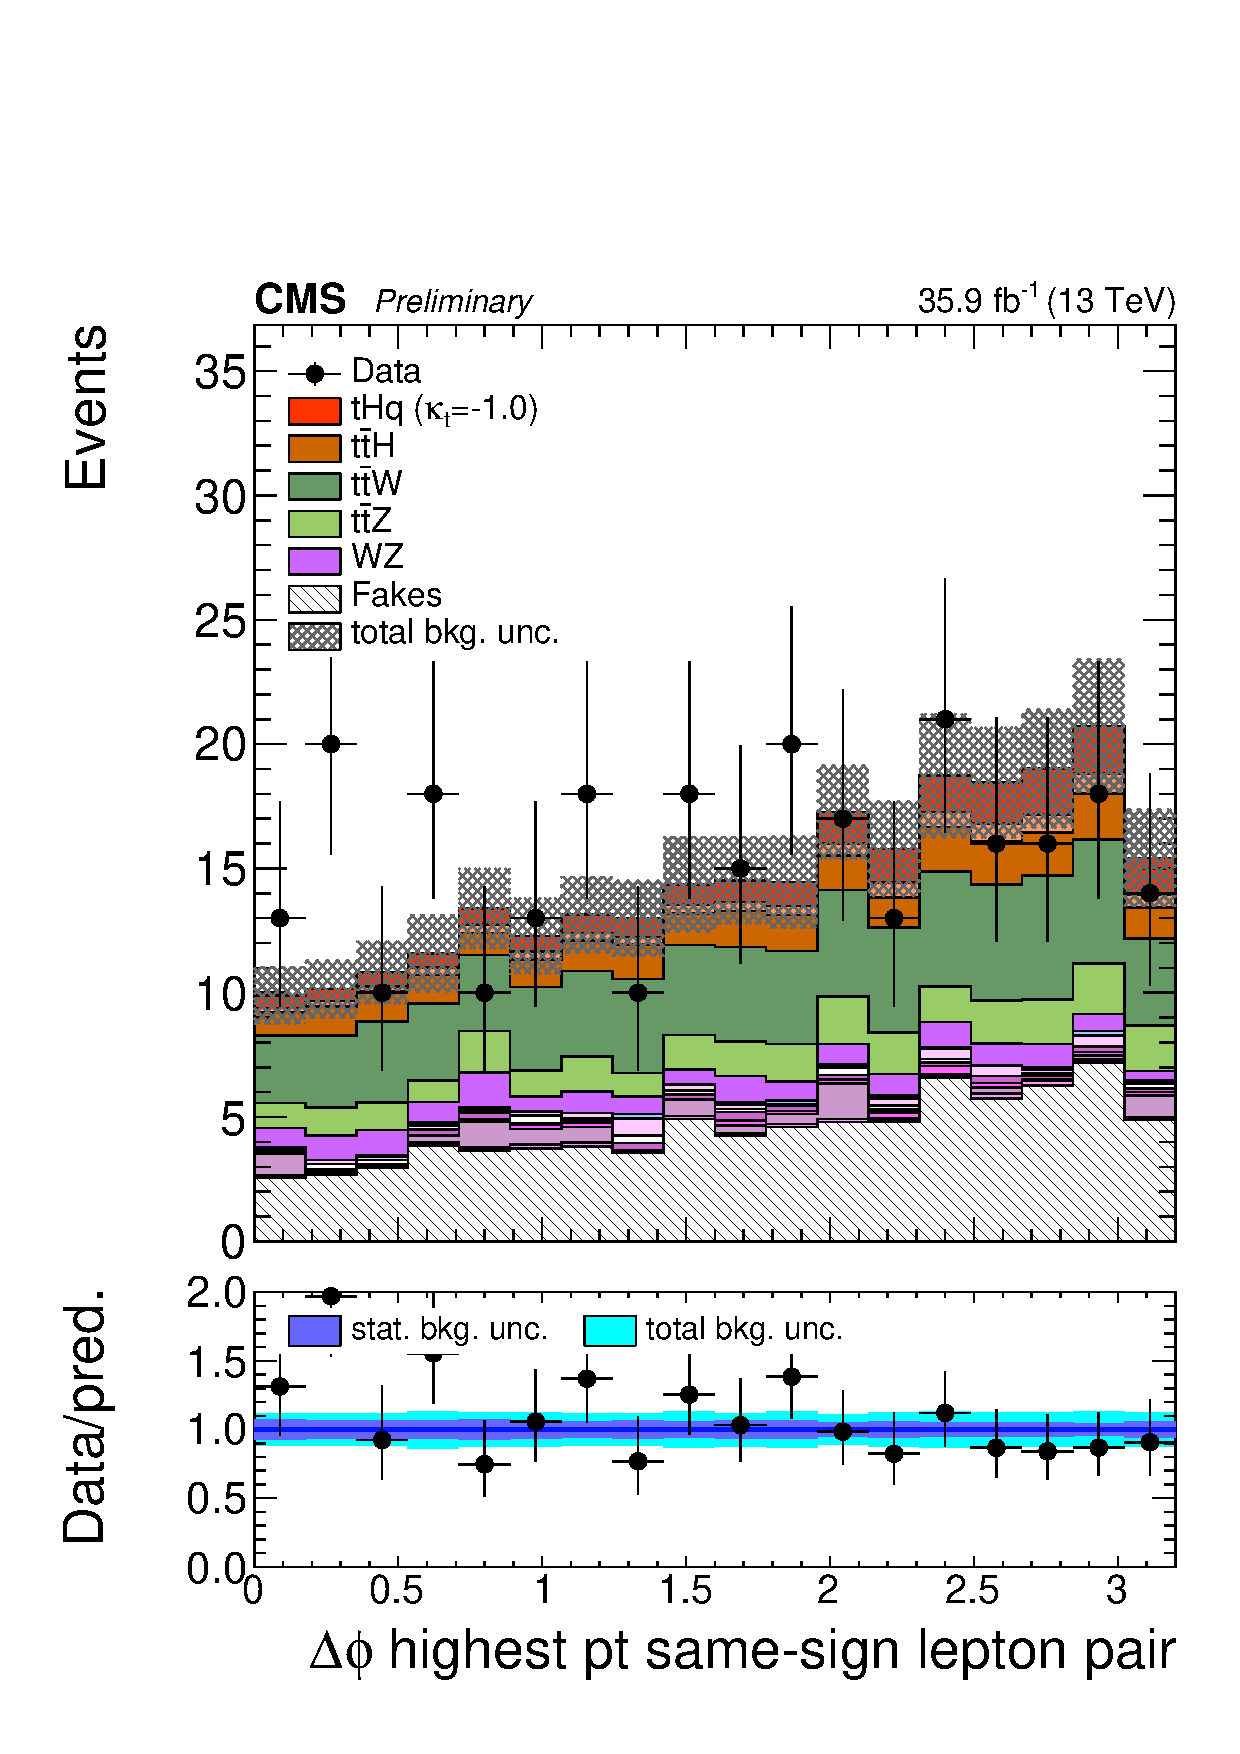
\includegraphics[width=0.22\textwidth]{figures/signalregion_2lss/mumu/dPhiHighestPtSSPair.pdf}
  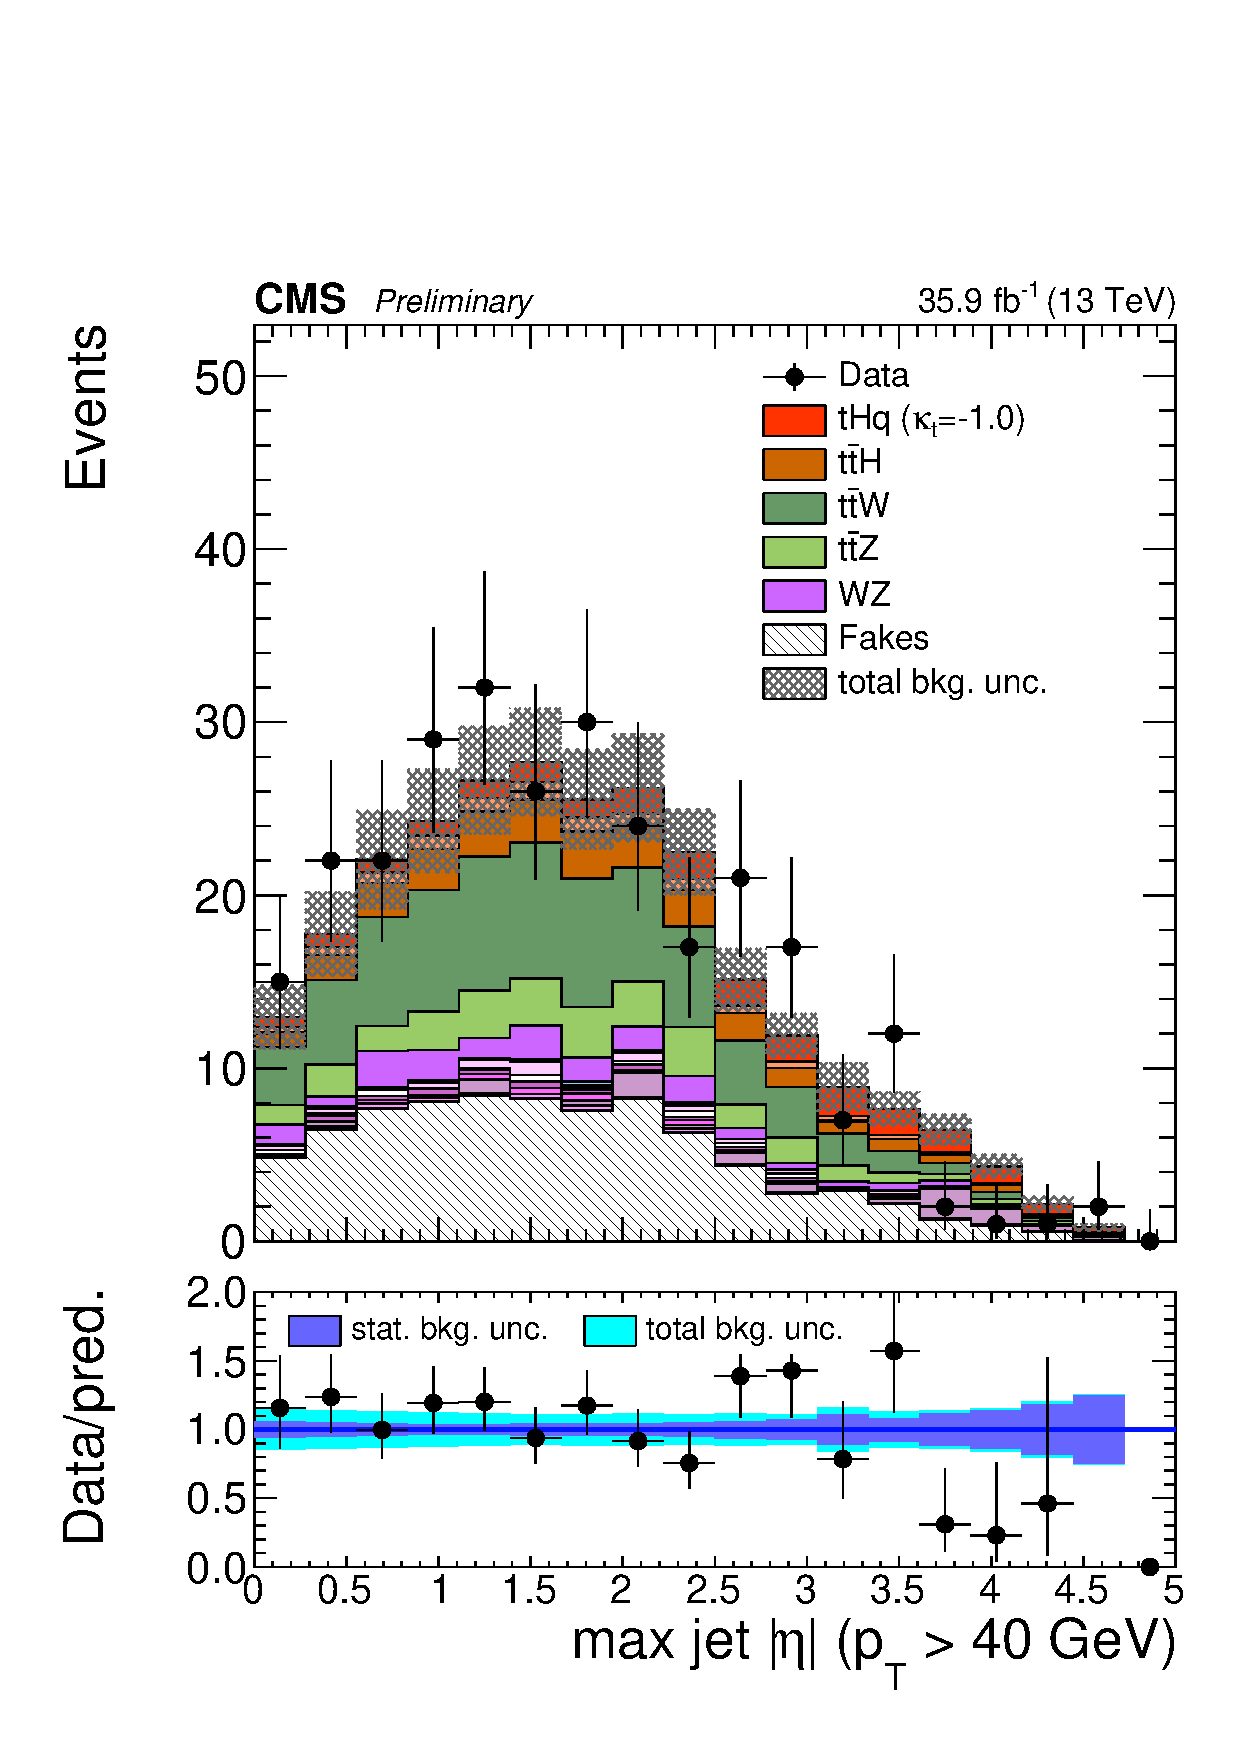
\includegraphics[width=0.22\textwidth]{figures/signalregion_2lss/mumu/maxEtaJet25_40.pdf}
  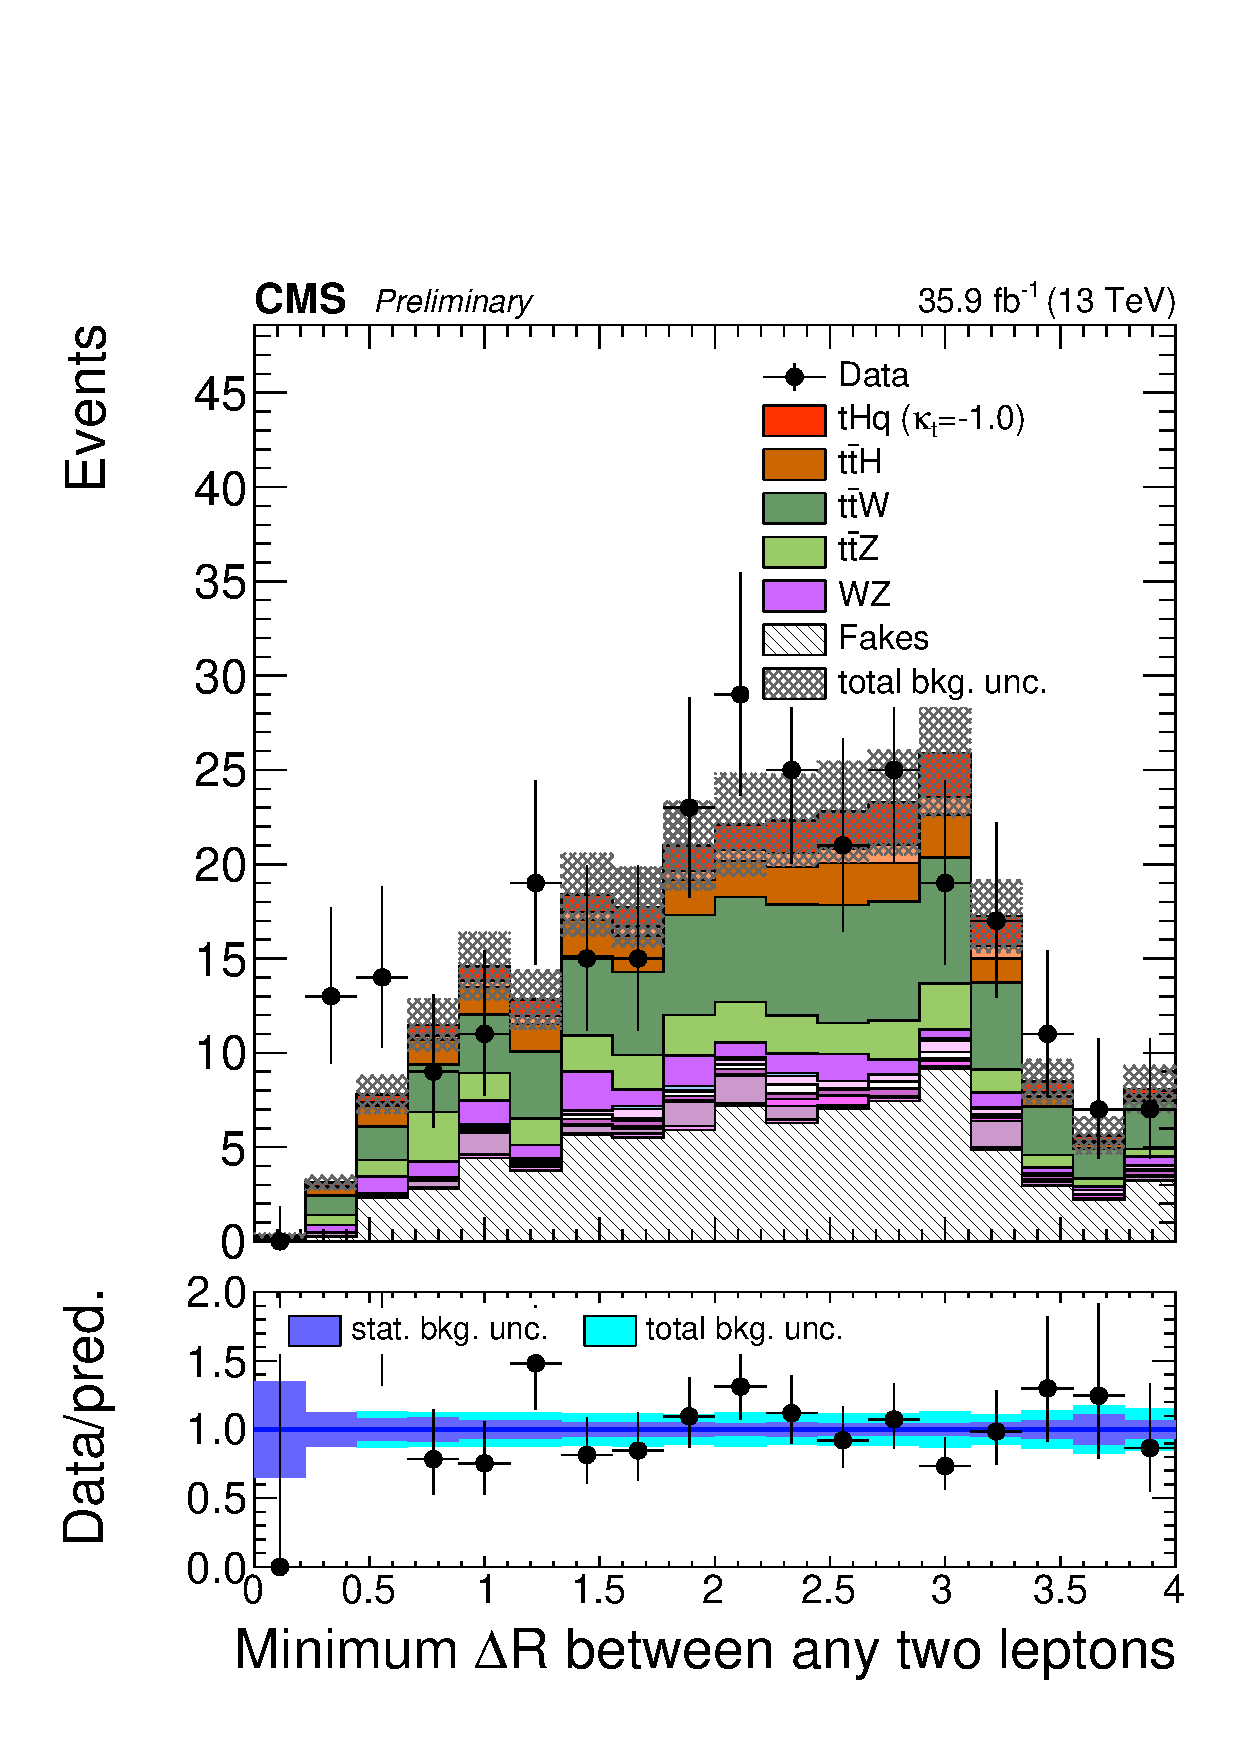
\includegraphics[width=0.22\textwidth]{figures/signalregion_2lss/mumu/minDRll.pdf} 
  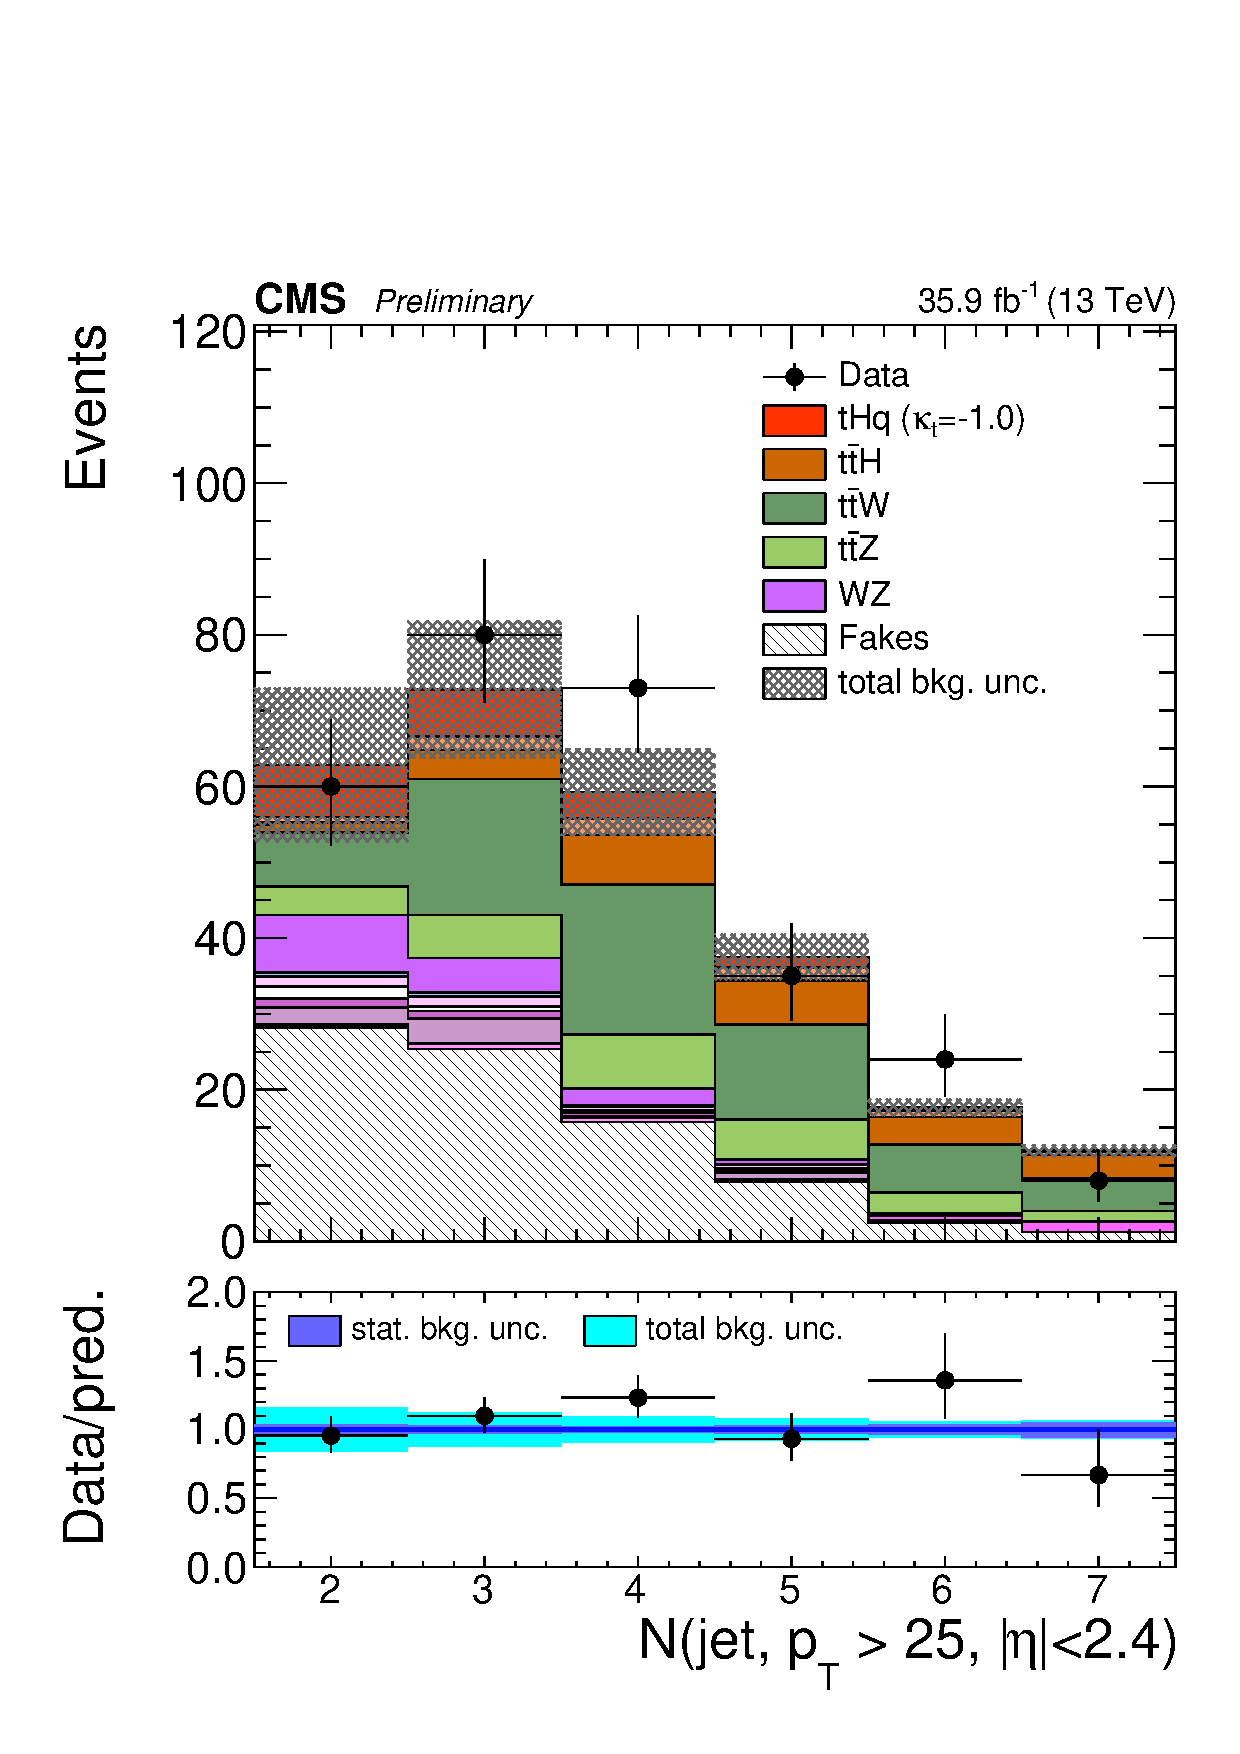
\includegraphics[width=0.22\textwidth]{figures/signalregion_2lss/mumu/nJet25.pdf} \\
  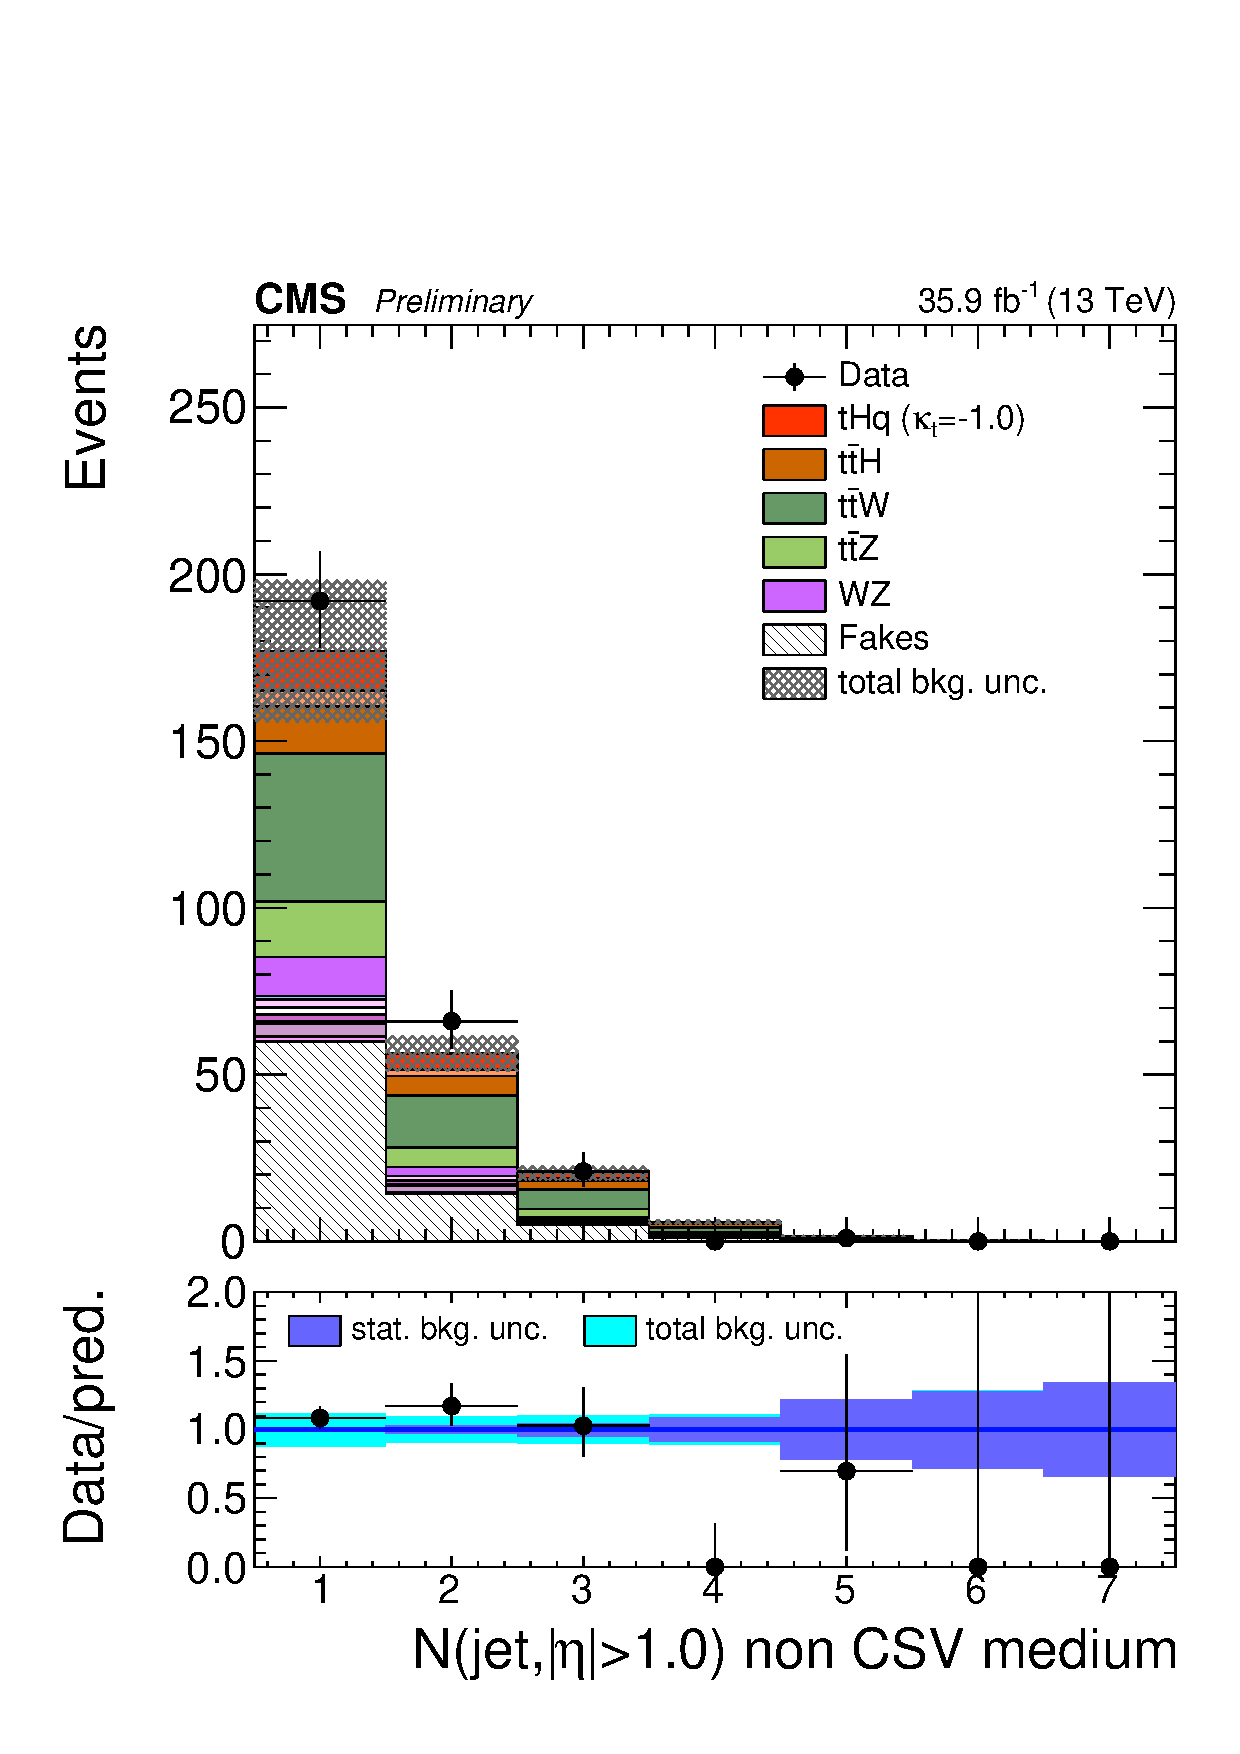
\includegraphics[width=0.22\textwidth]{figures/signalregion_2lss/mumu/nJetEta1_40.pdf}
  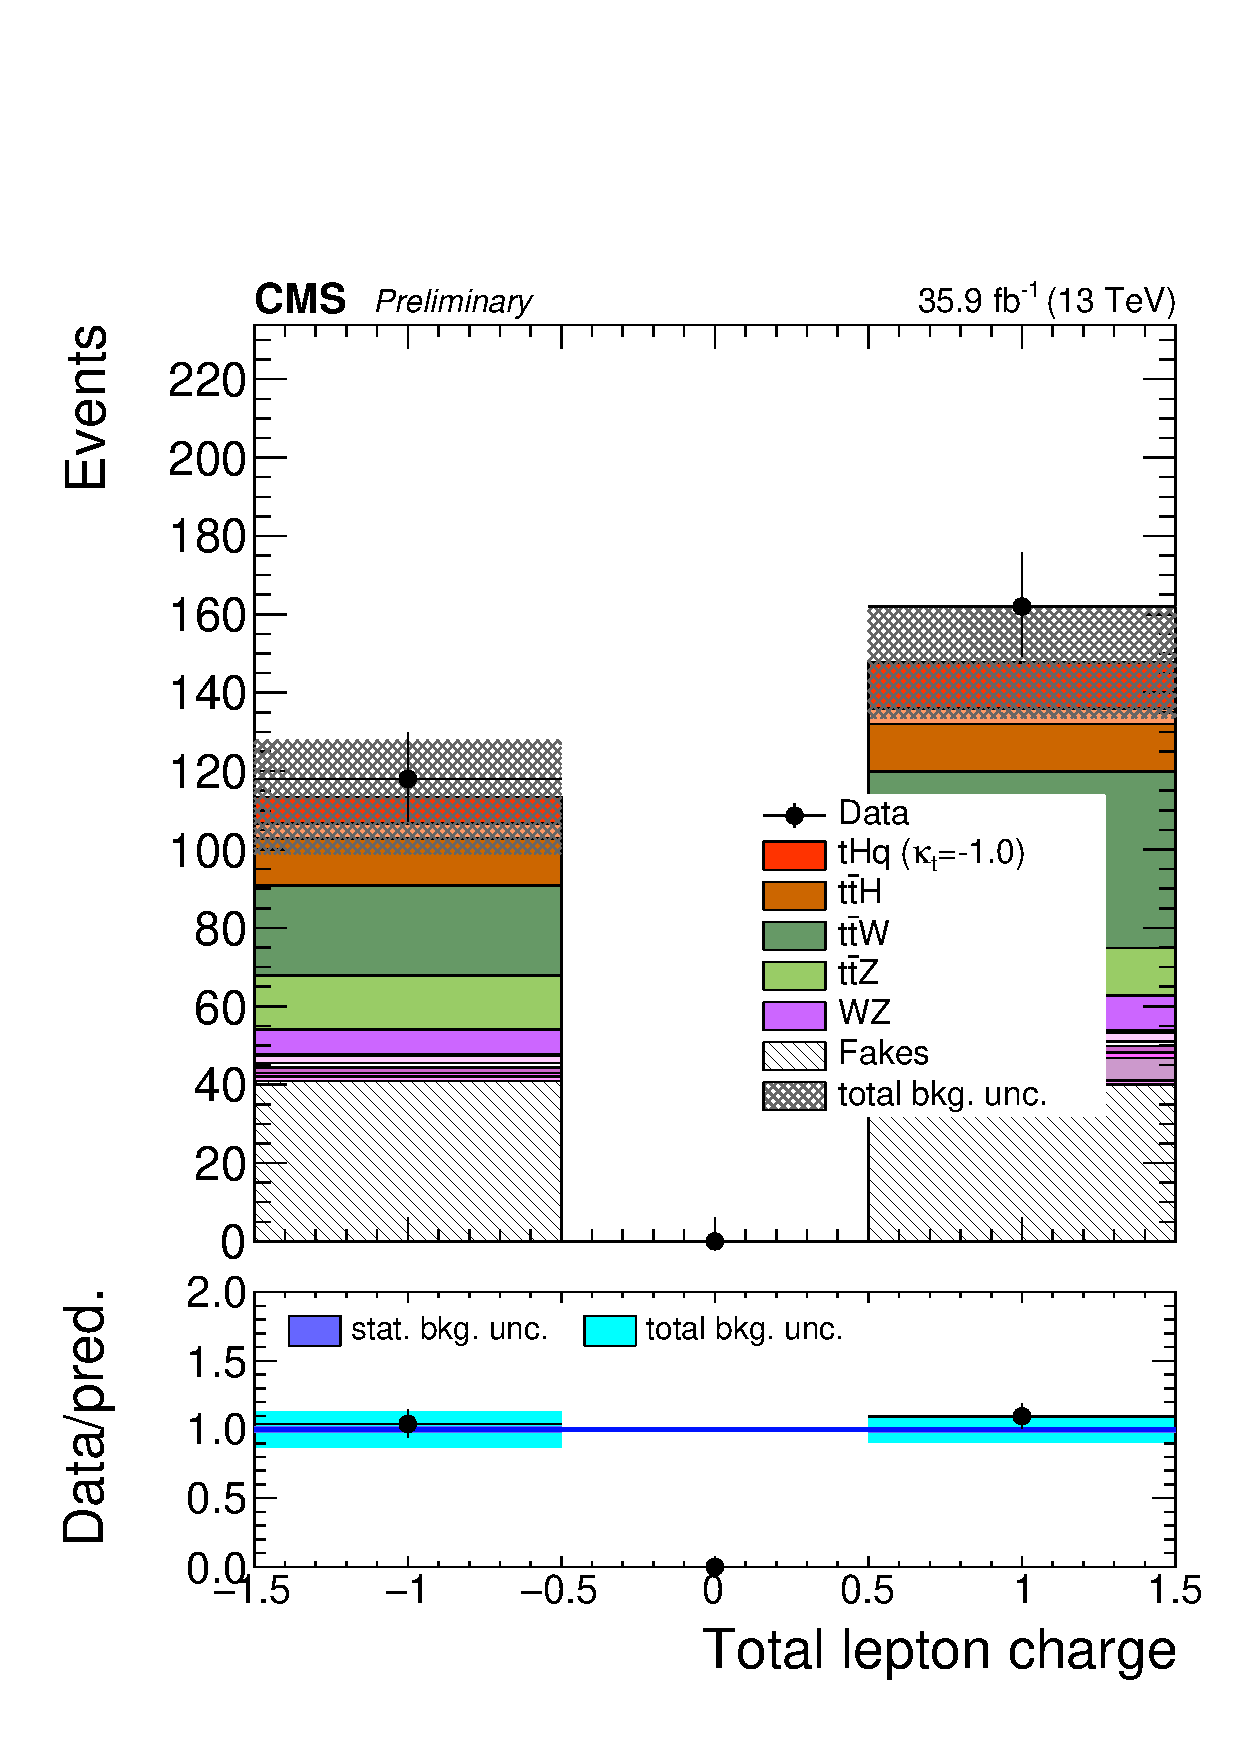
\includegraphics[width=0.22\textwidth]{figures/signalregion_2lss/mumu/totCharge.pdf}
\caption{Distributions of input variables to the BDT for signal discrimination, in \mumu\ channel, normalized to their cross section and to 35.9\fbinv.}
\label{fig:input_vars_2lss_xsec_mumu}
\end{figure}

\begin{figure} [!h]
  \centering
  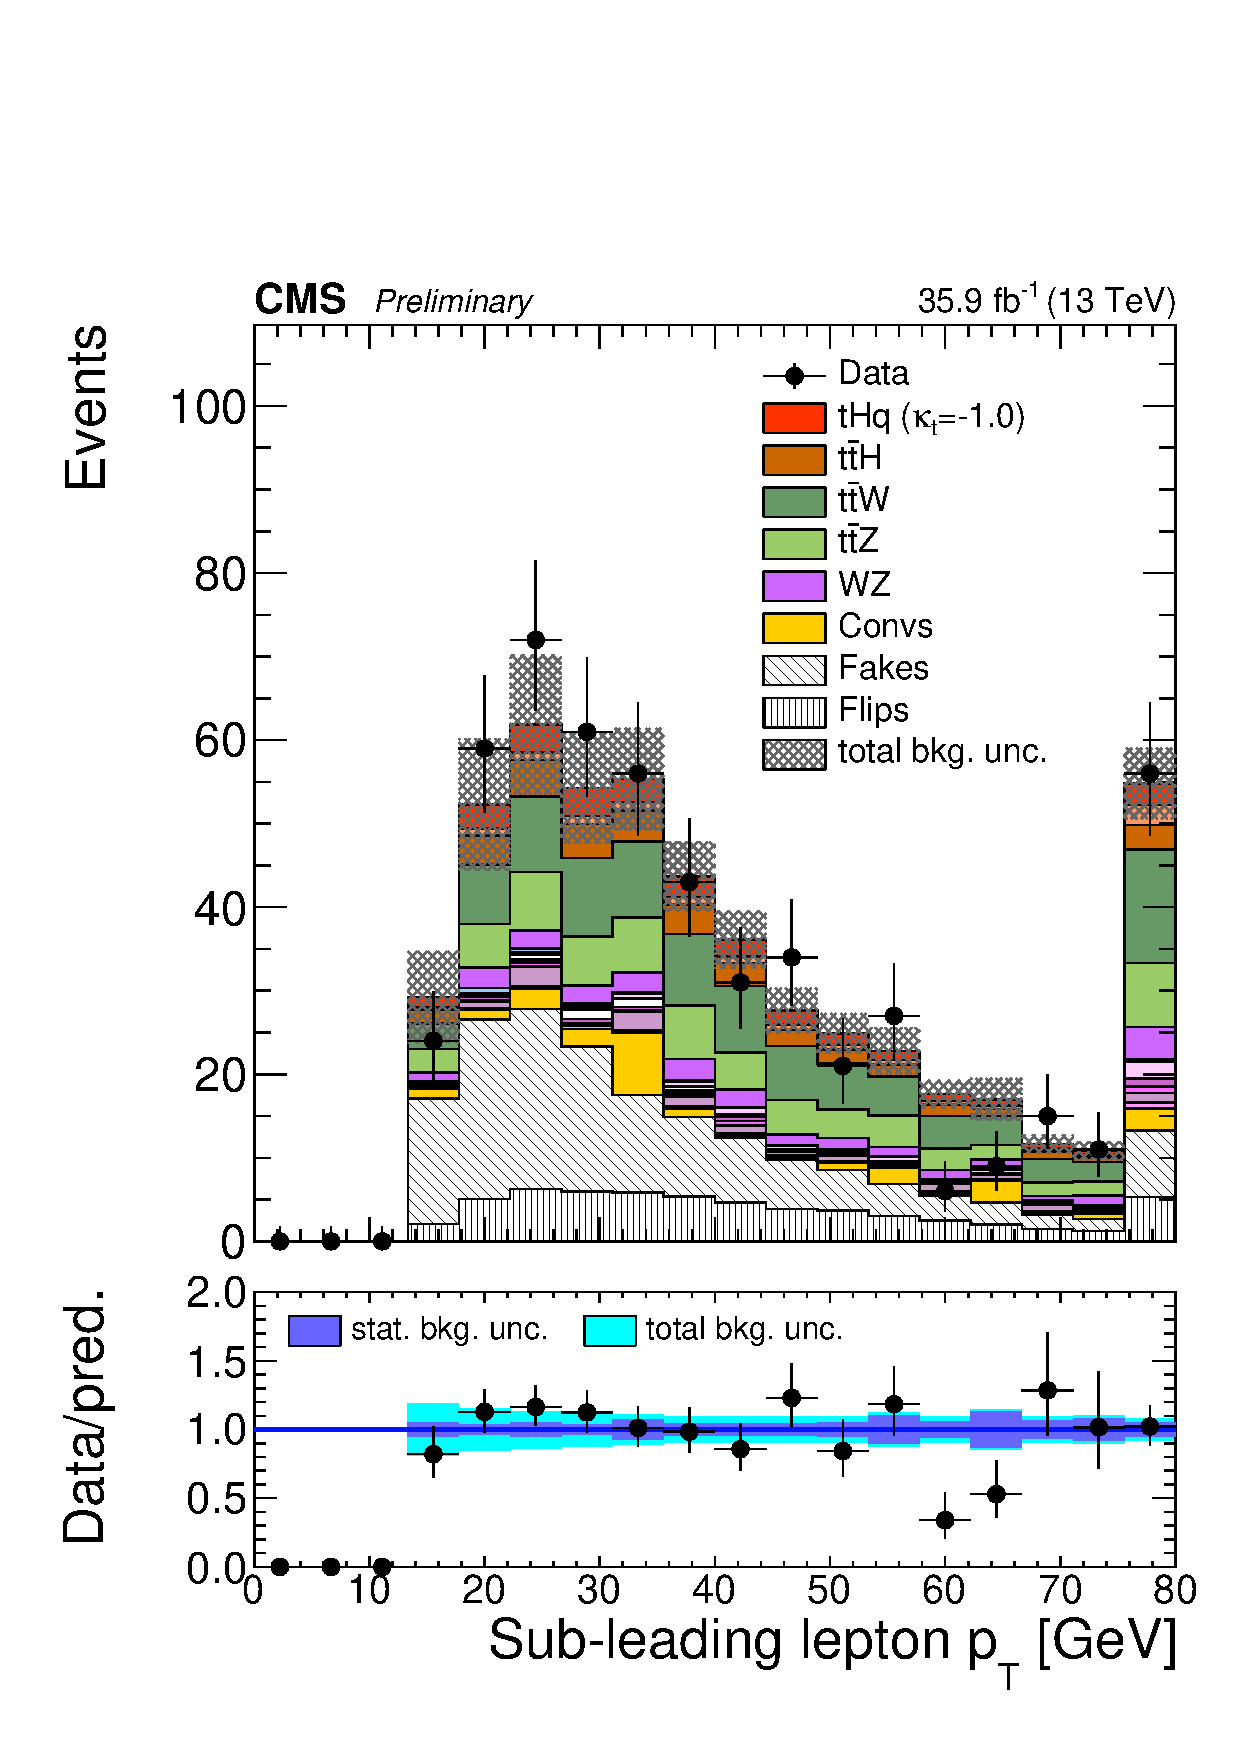
\includegraphics[width=0.22\textwidth]{figures/signalregion_2lss/emu/Lep2Pt.pdf}
  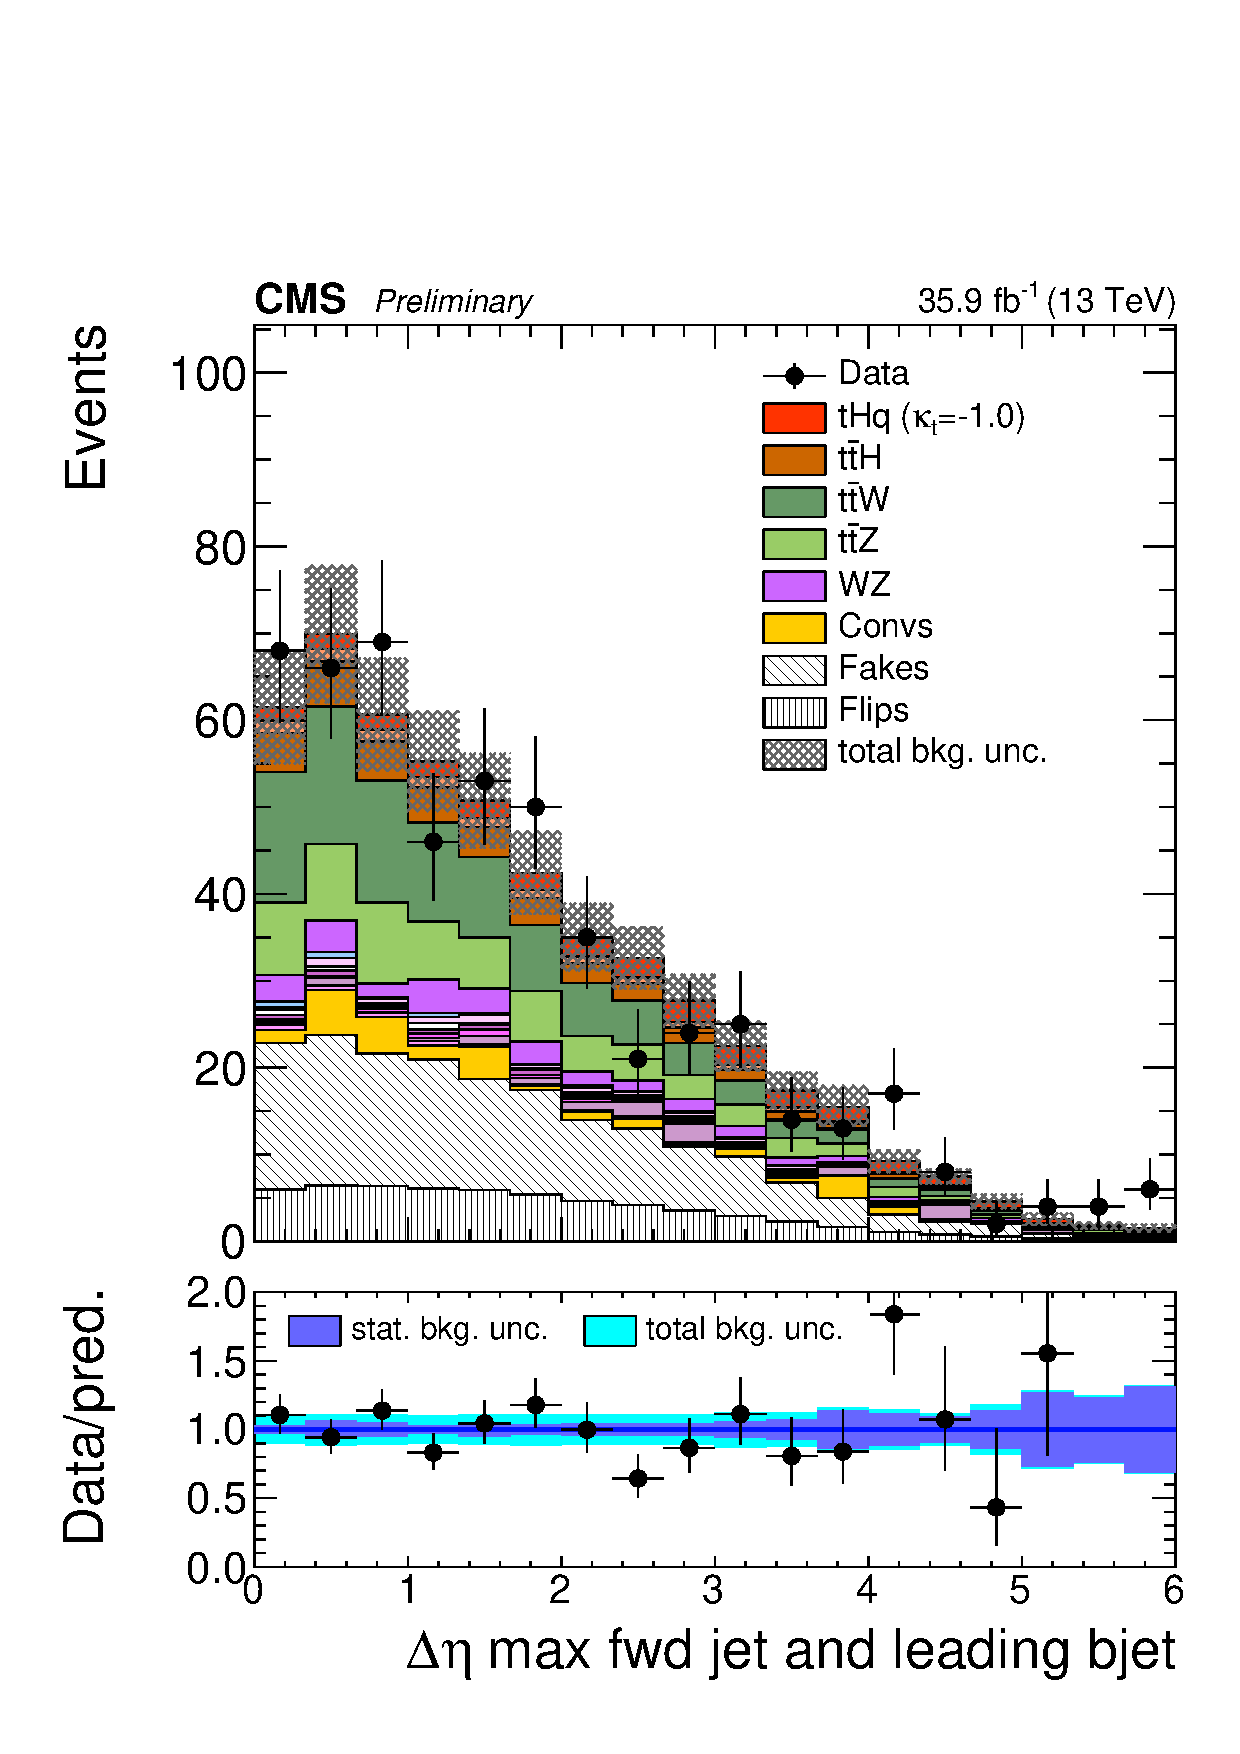
\includegraphics[width=0.22\textwidth]{figures/signalregion_2lss/emu/dEtaFwdJetBJet_40.pdf}
  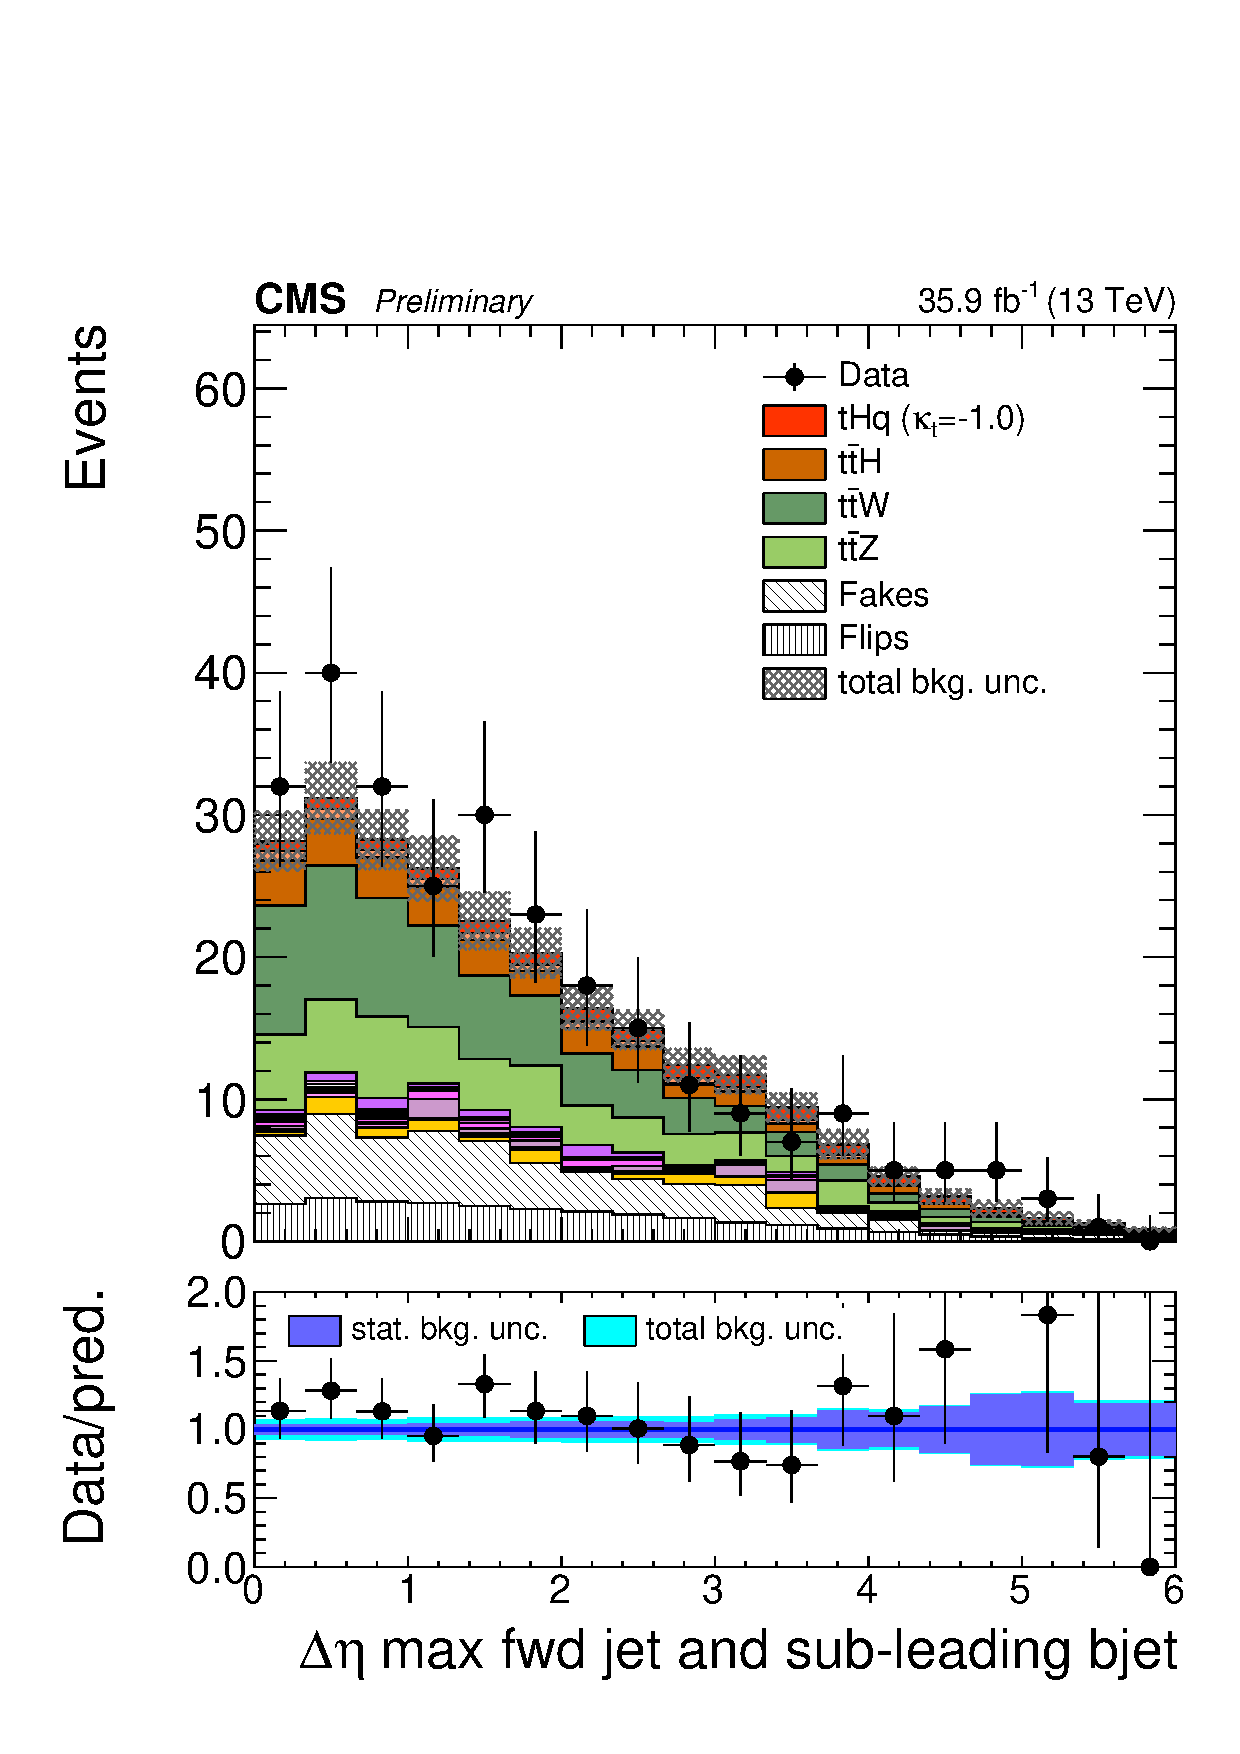
\includegraphics[width=0.22\textwidth]{figures/signalregion_2lss/emu/dEtaFwdJet2BJet_40.pdf}
  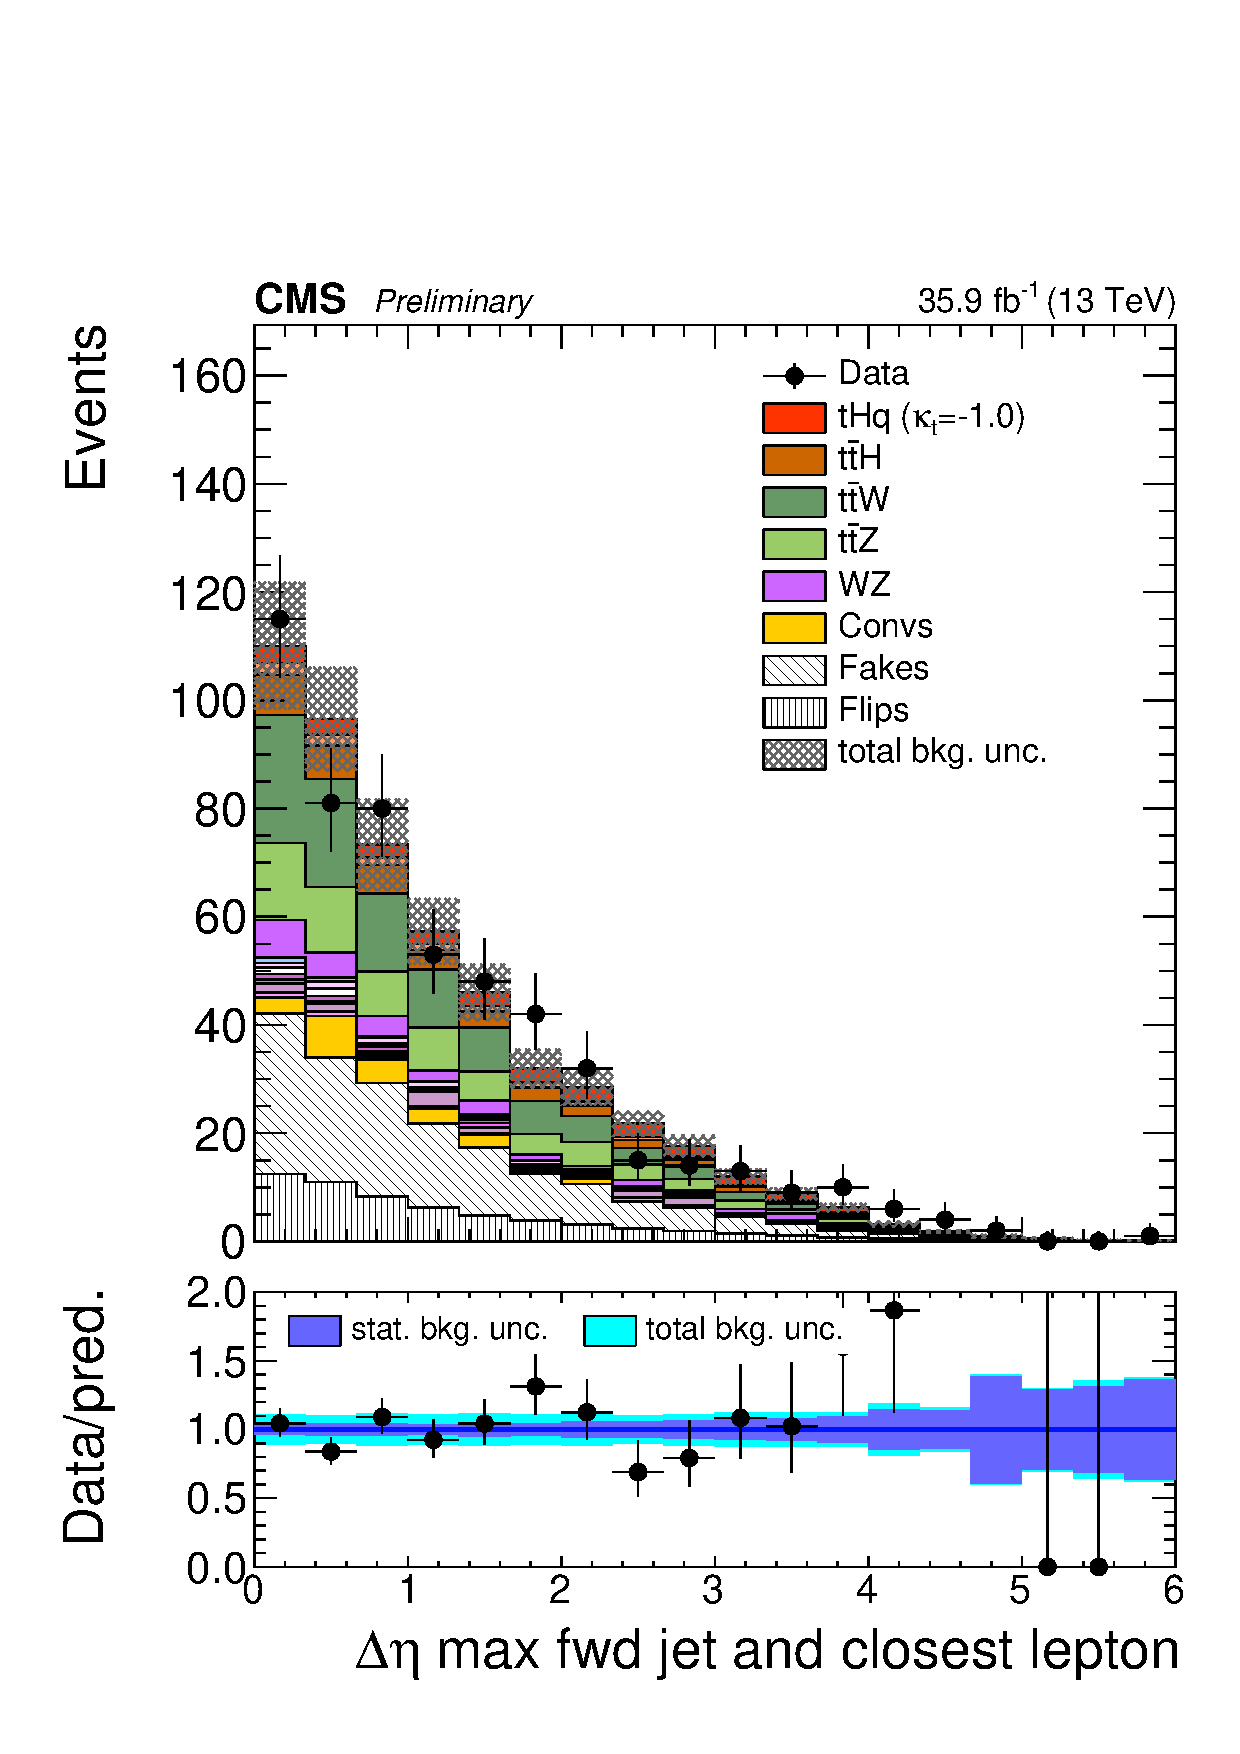
\includegraphics[width=0.22\textwidth]{figures/signalregion_2lss/emu/dEtaFwdJetClosestLep_40.pdf} \\
  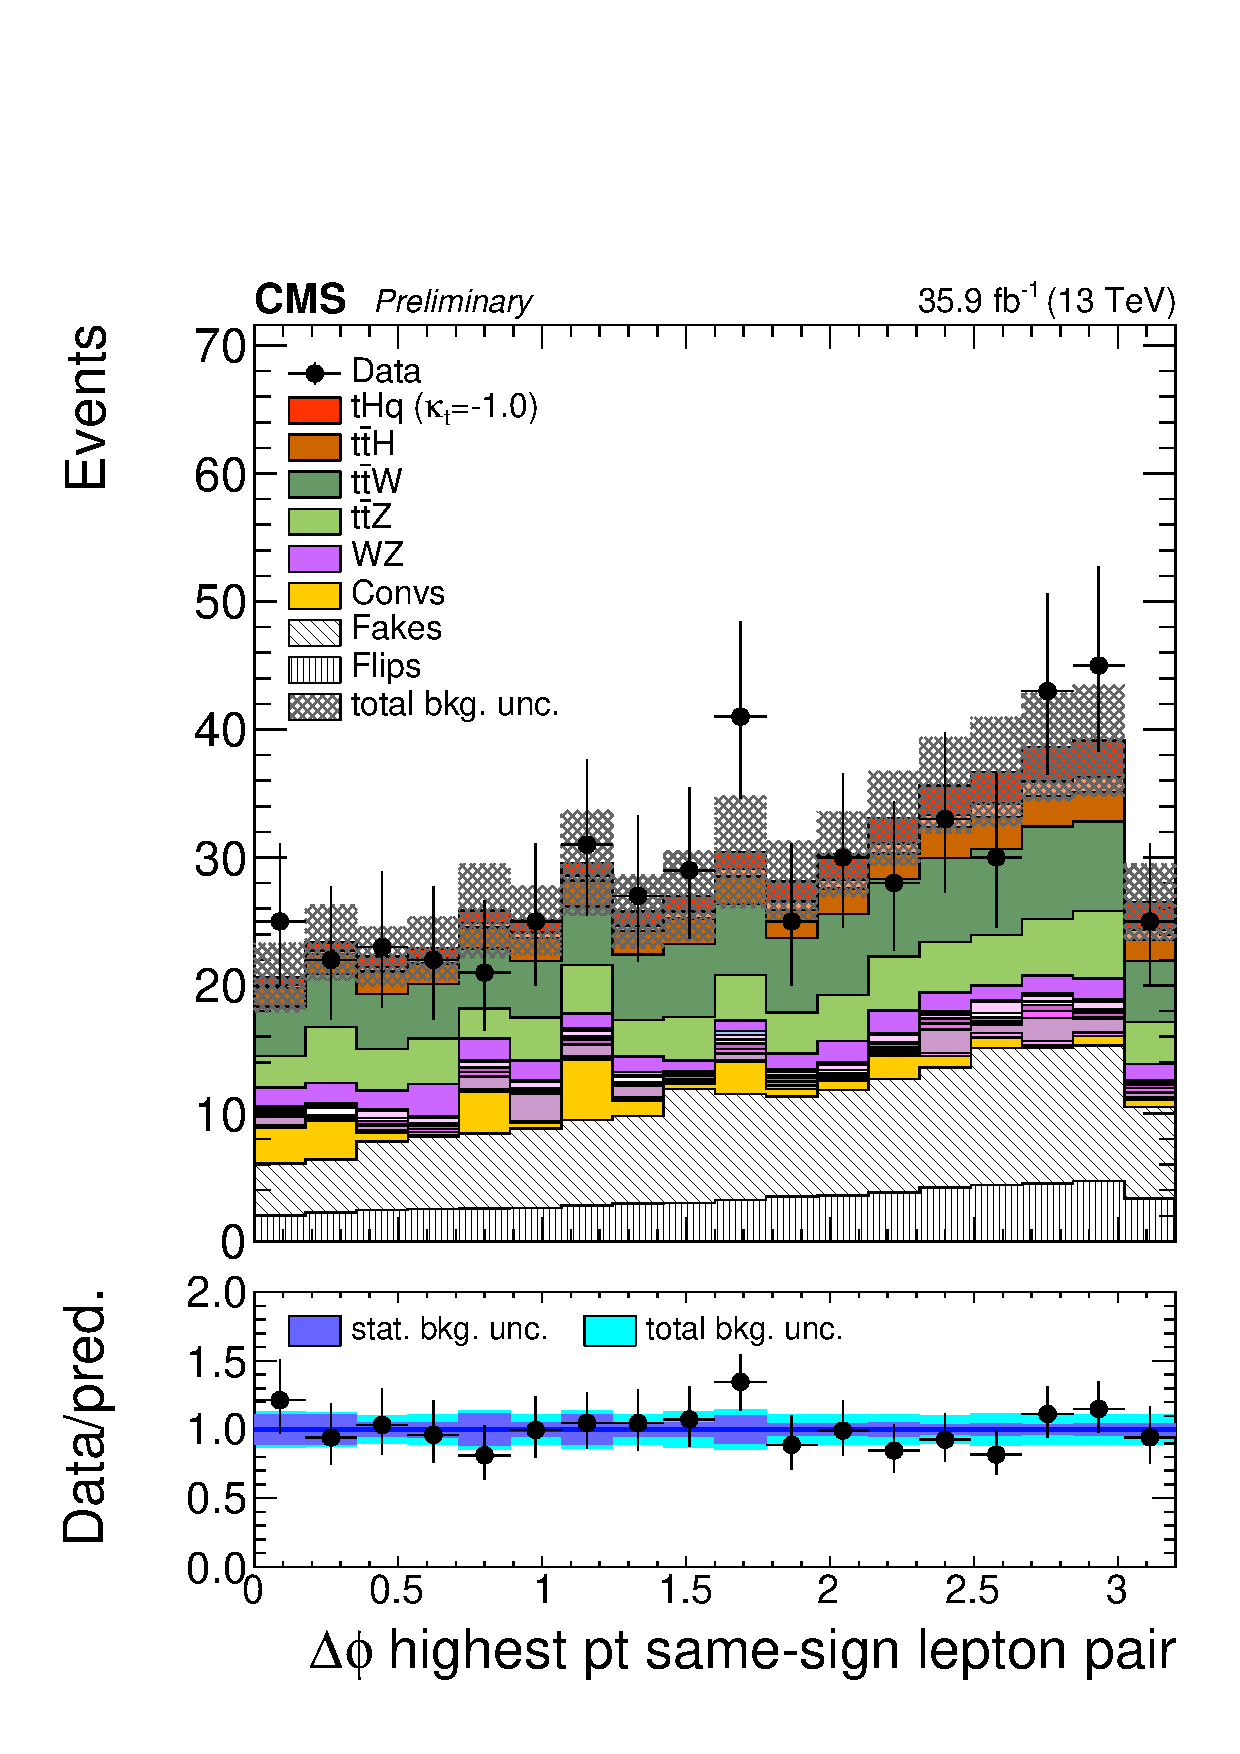
\includegraphics[width=0.22\textwidth]{figures/signalregion_2lss/emu/dPhiHighestPtSSPair.pdf}
  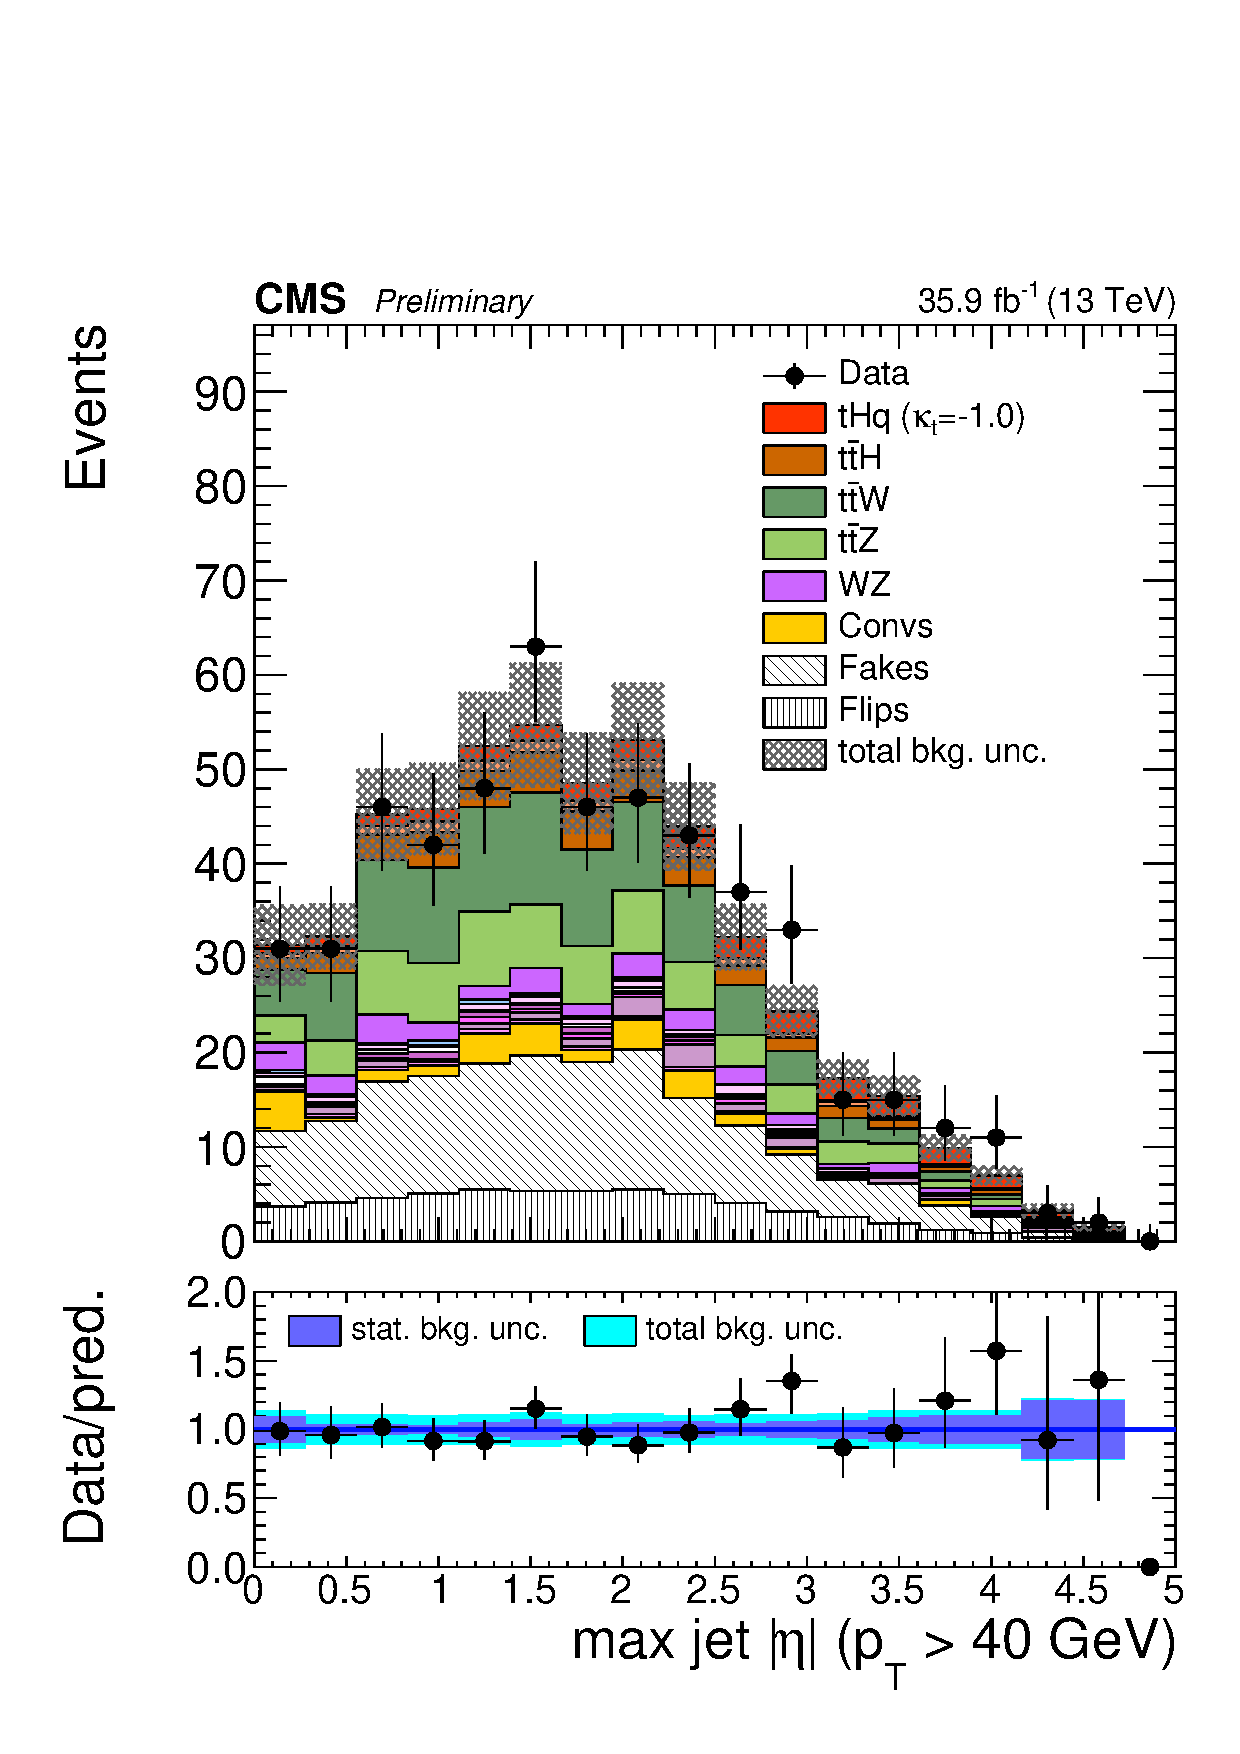
\includegraphics[width=0.22\textwidth]{figures/signalregion_2lss/emu/maxEtaJet25_40.pdf}
  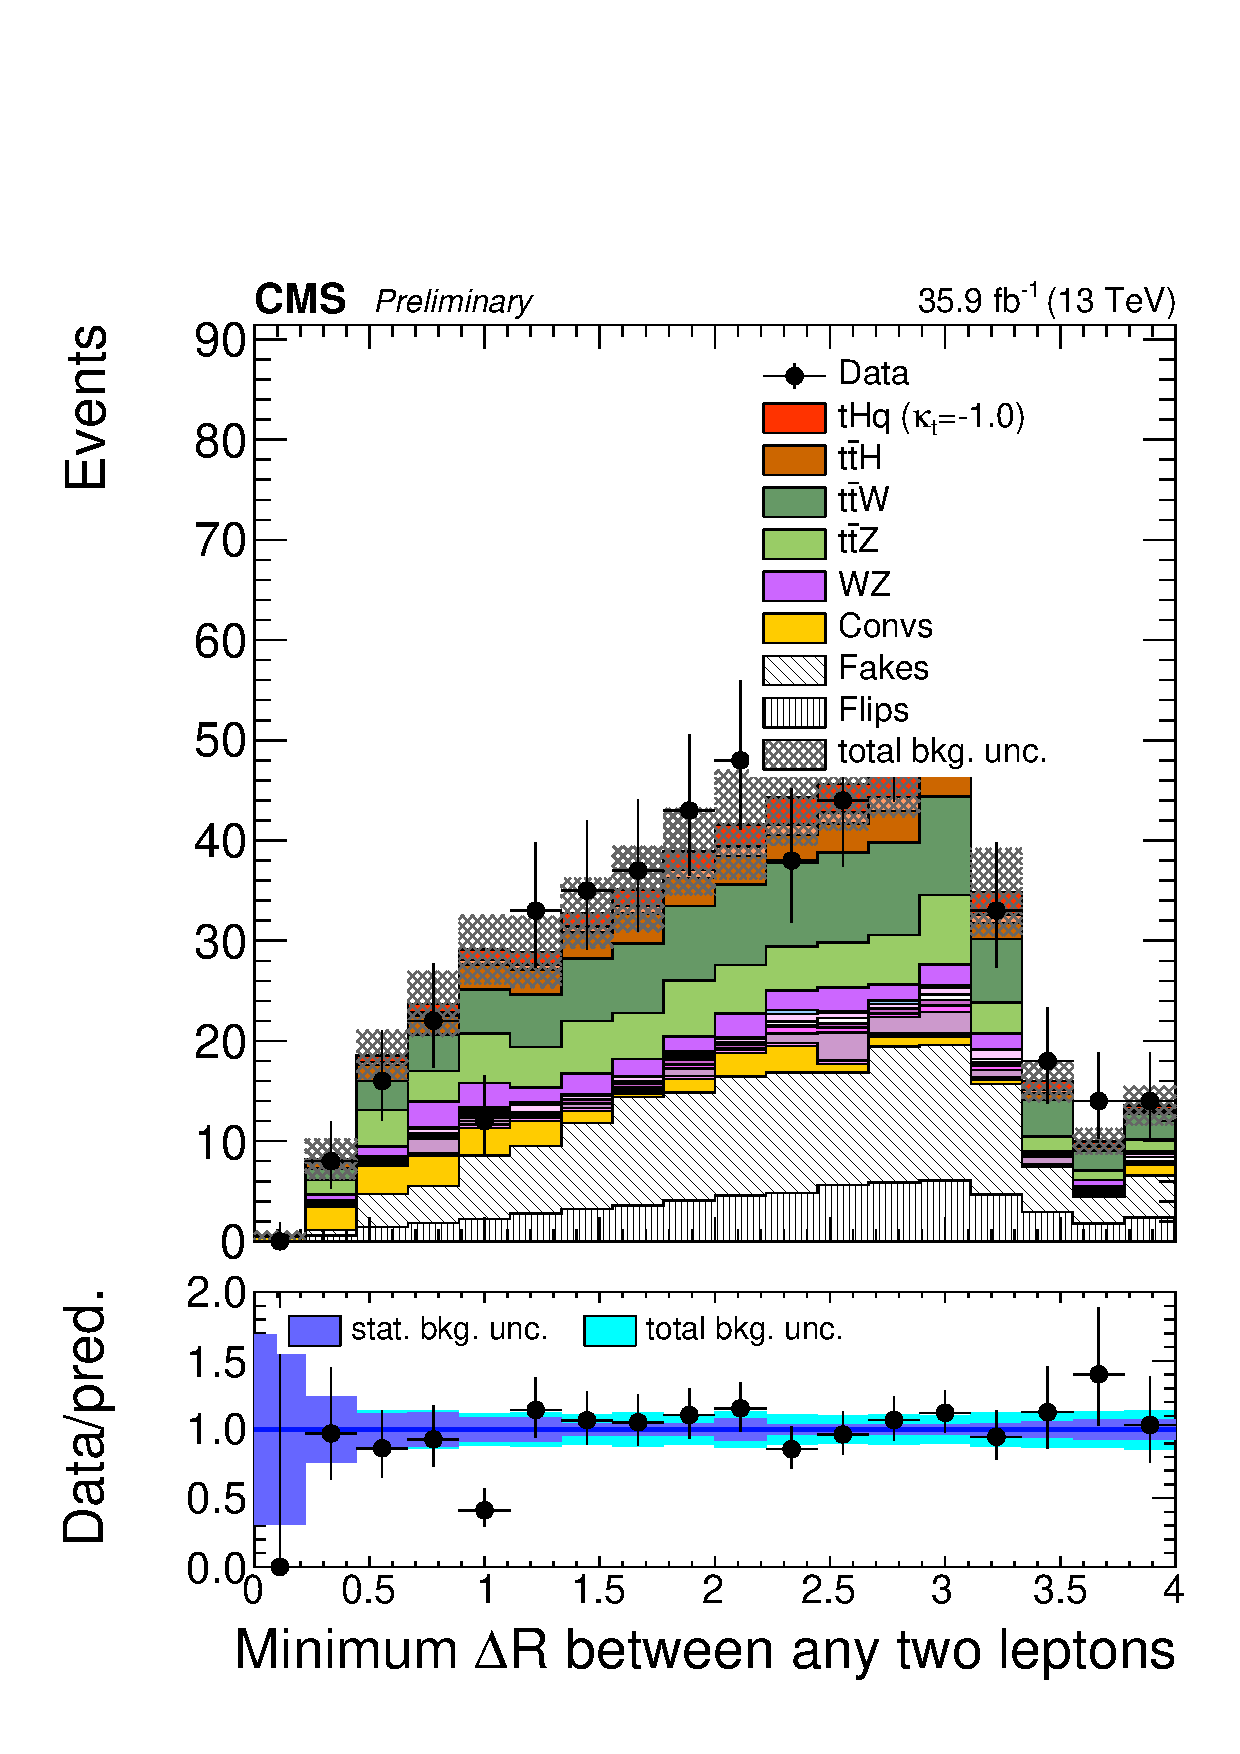
\includegraphics[width=0.22\textwidth]{figures/signalregion_2lss/emu/minDRll.pdf} 
  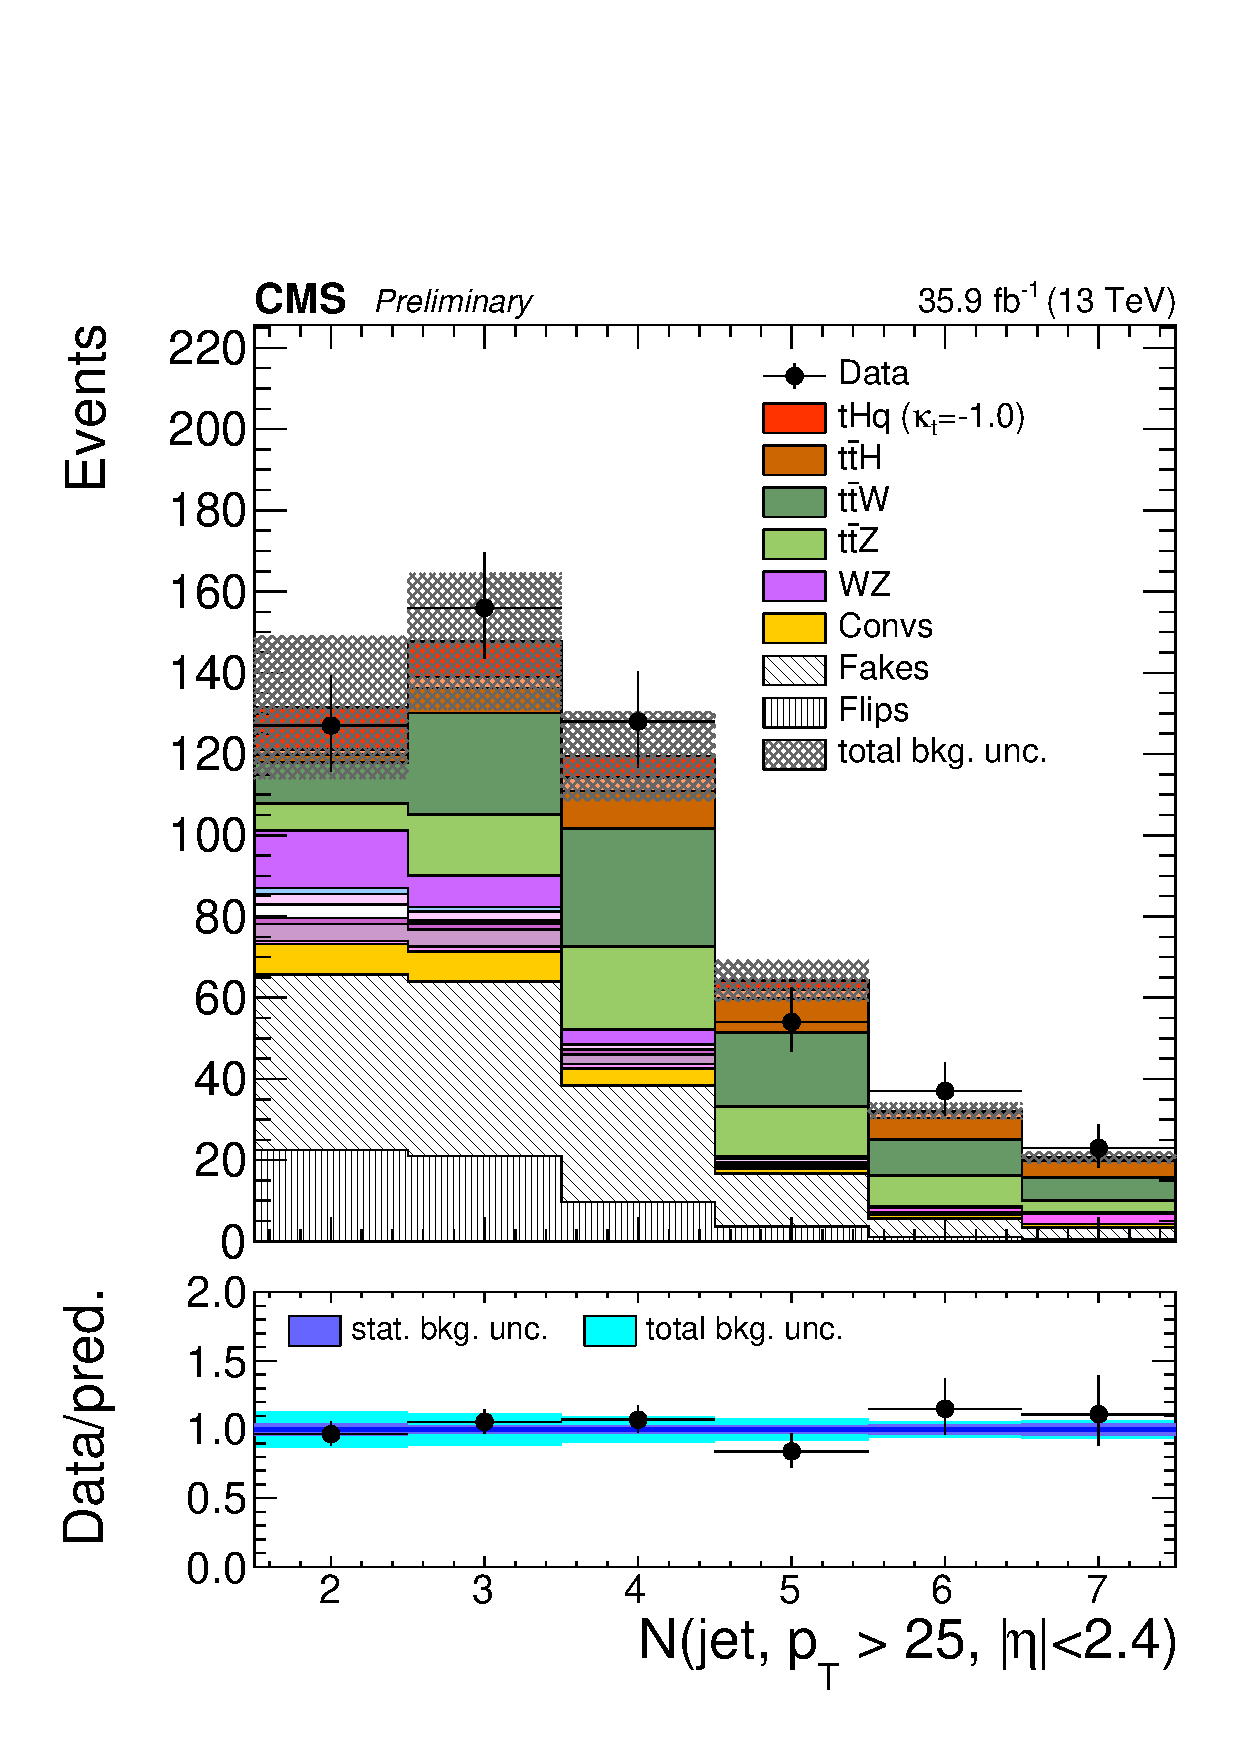
\includegraphics[width=0.22\textwidth]{figures/signalregion_2lss/emu/nJet25.pdf} \\
  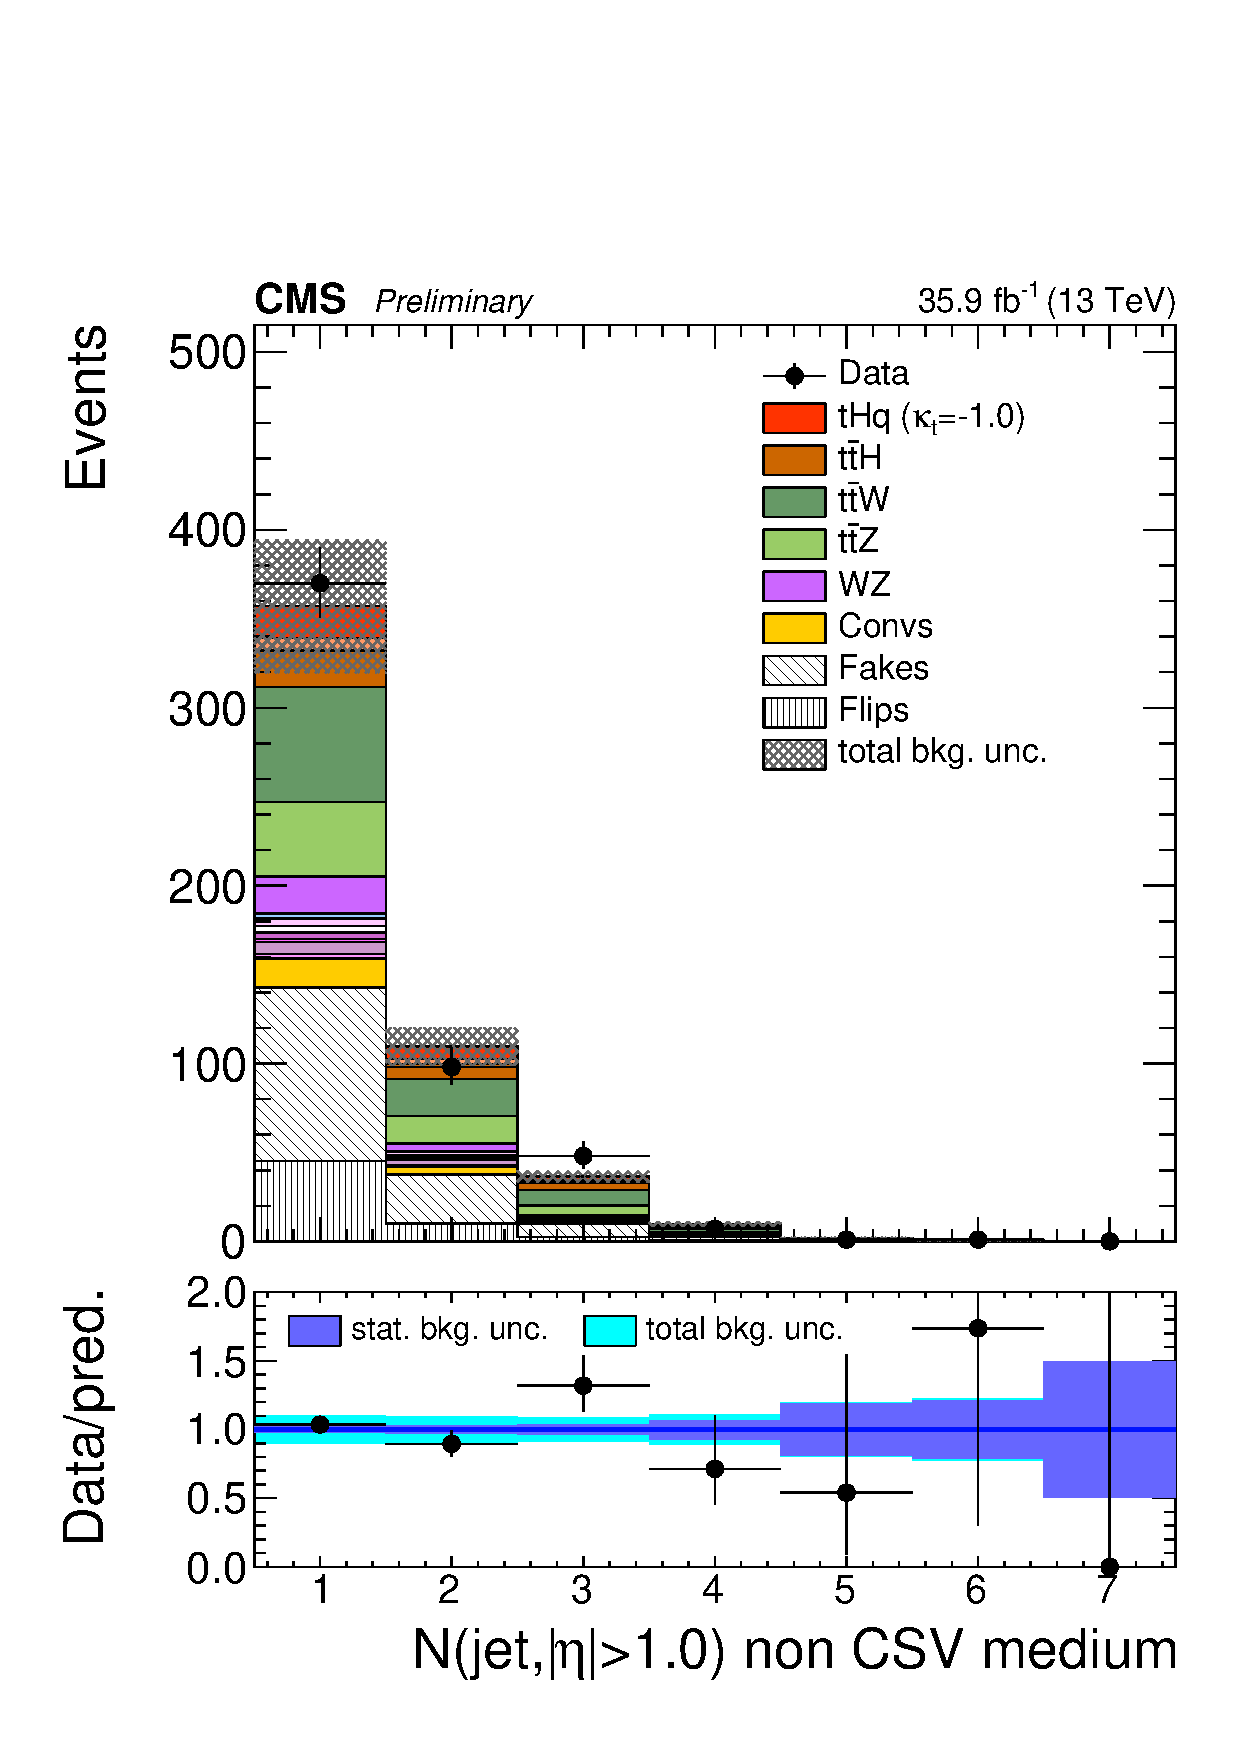
\includegraphics[width=0.22\textwidth]{figures/signalregion_2lss/emu/nJetEta1_40.pdf}
  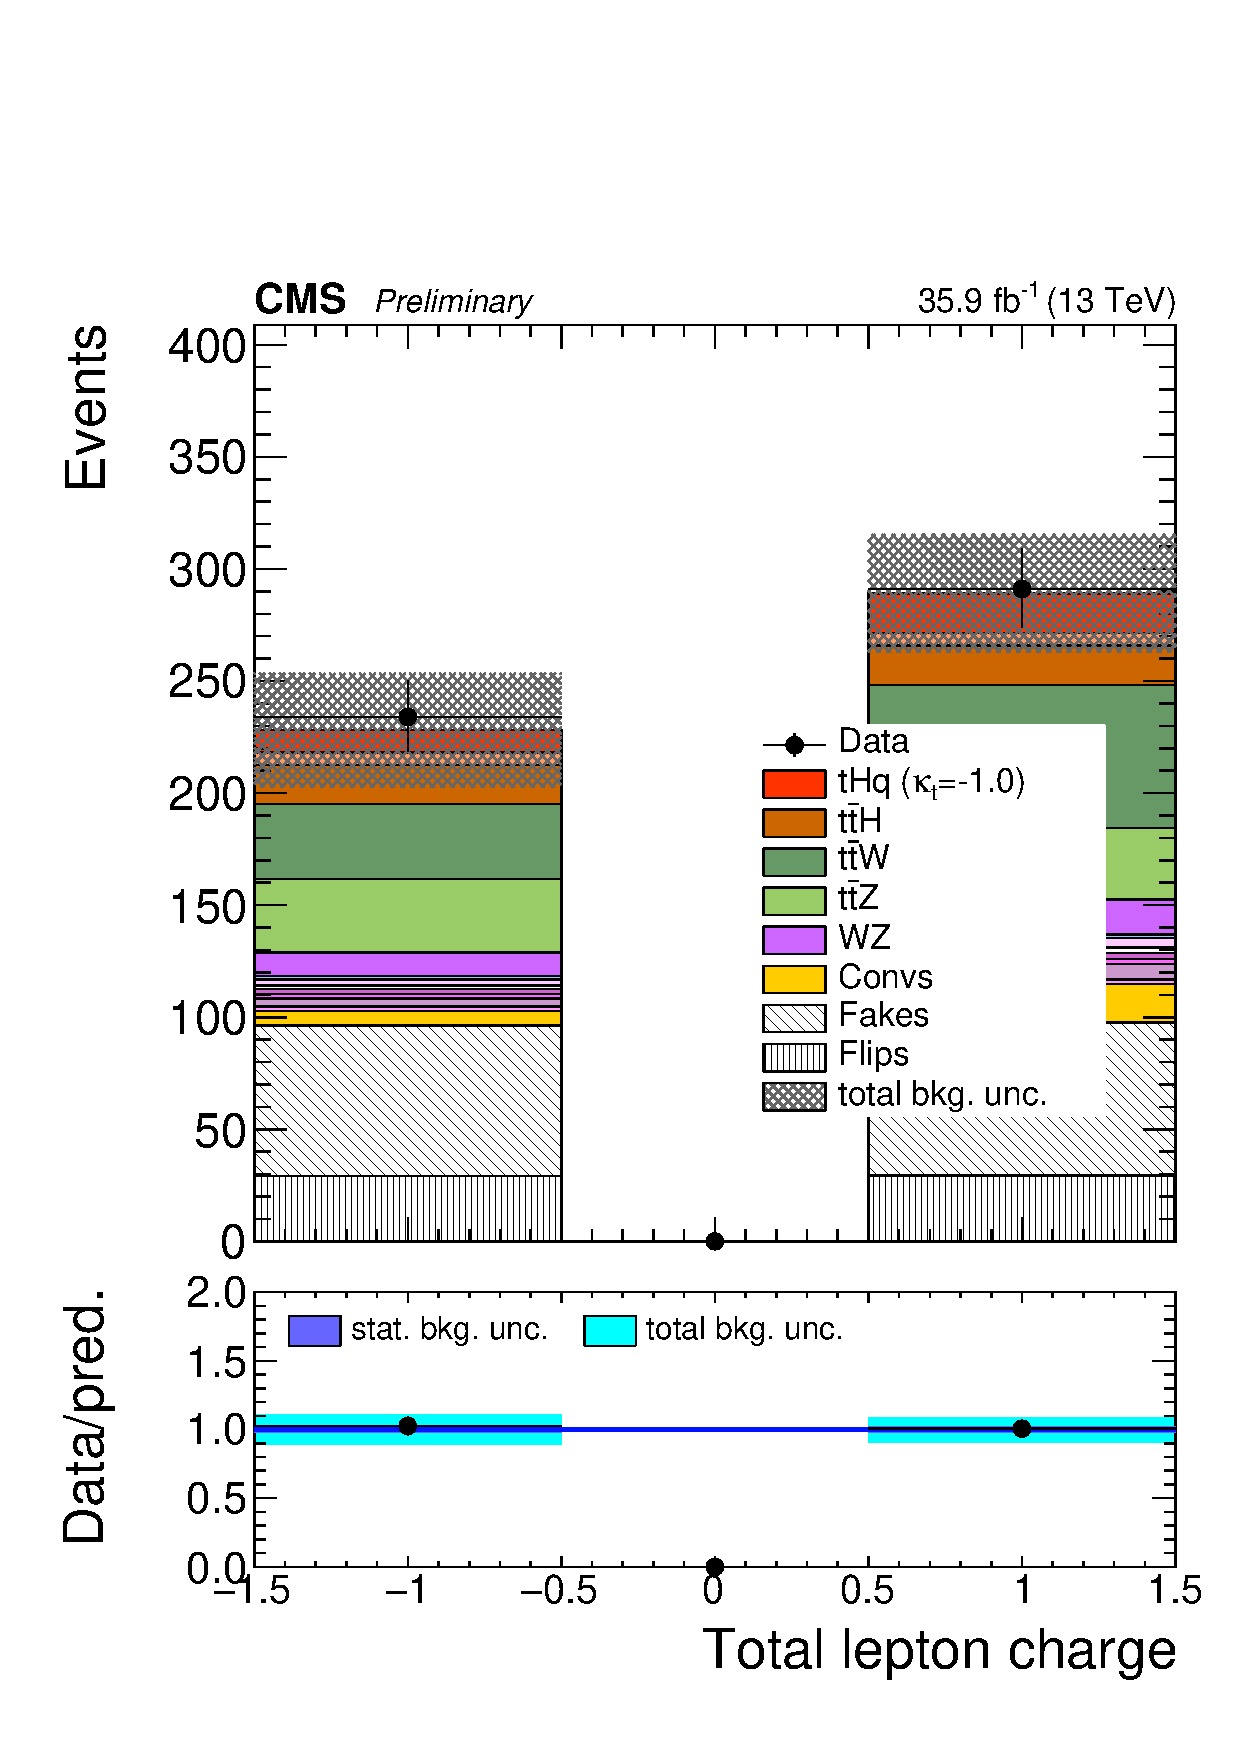
\includegraphics[width=0.22\textwidth]{figures/signalregion_2lss/emu/totCharge.pdf}
\caption{Distributions of input variables to the BDT for signal discrimination, in $e^{\pm}\mu^{\pm}$ channel, normalized to their cross section and to 35.9\fbinv.}
\label{fig:input_vars_2lss_xsec_emu}
\end{figure}

\begin{figure} [!h]
  \centering
  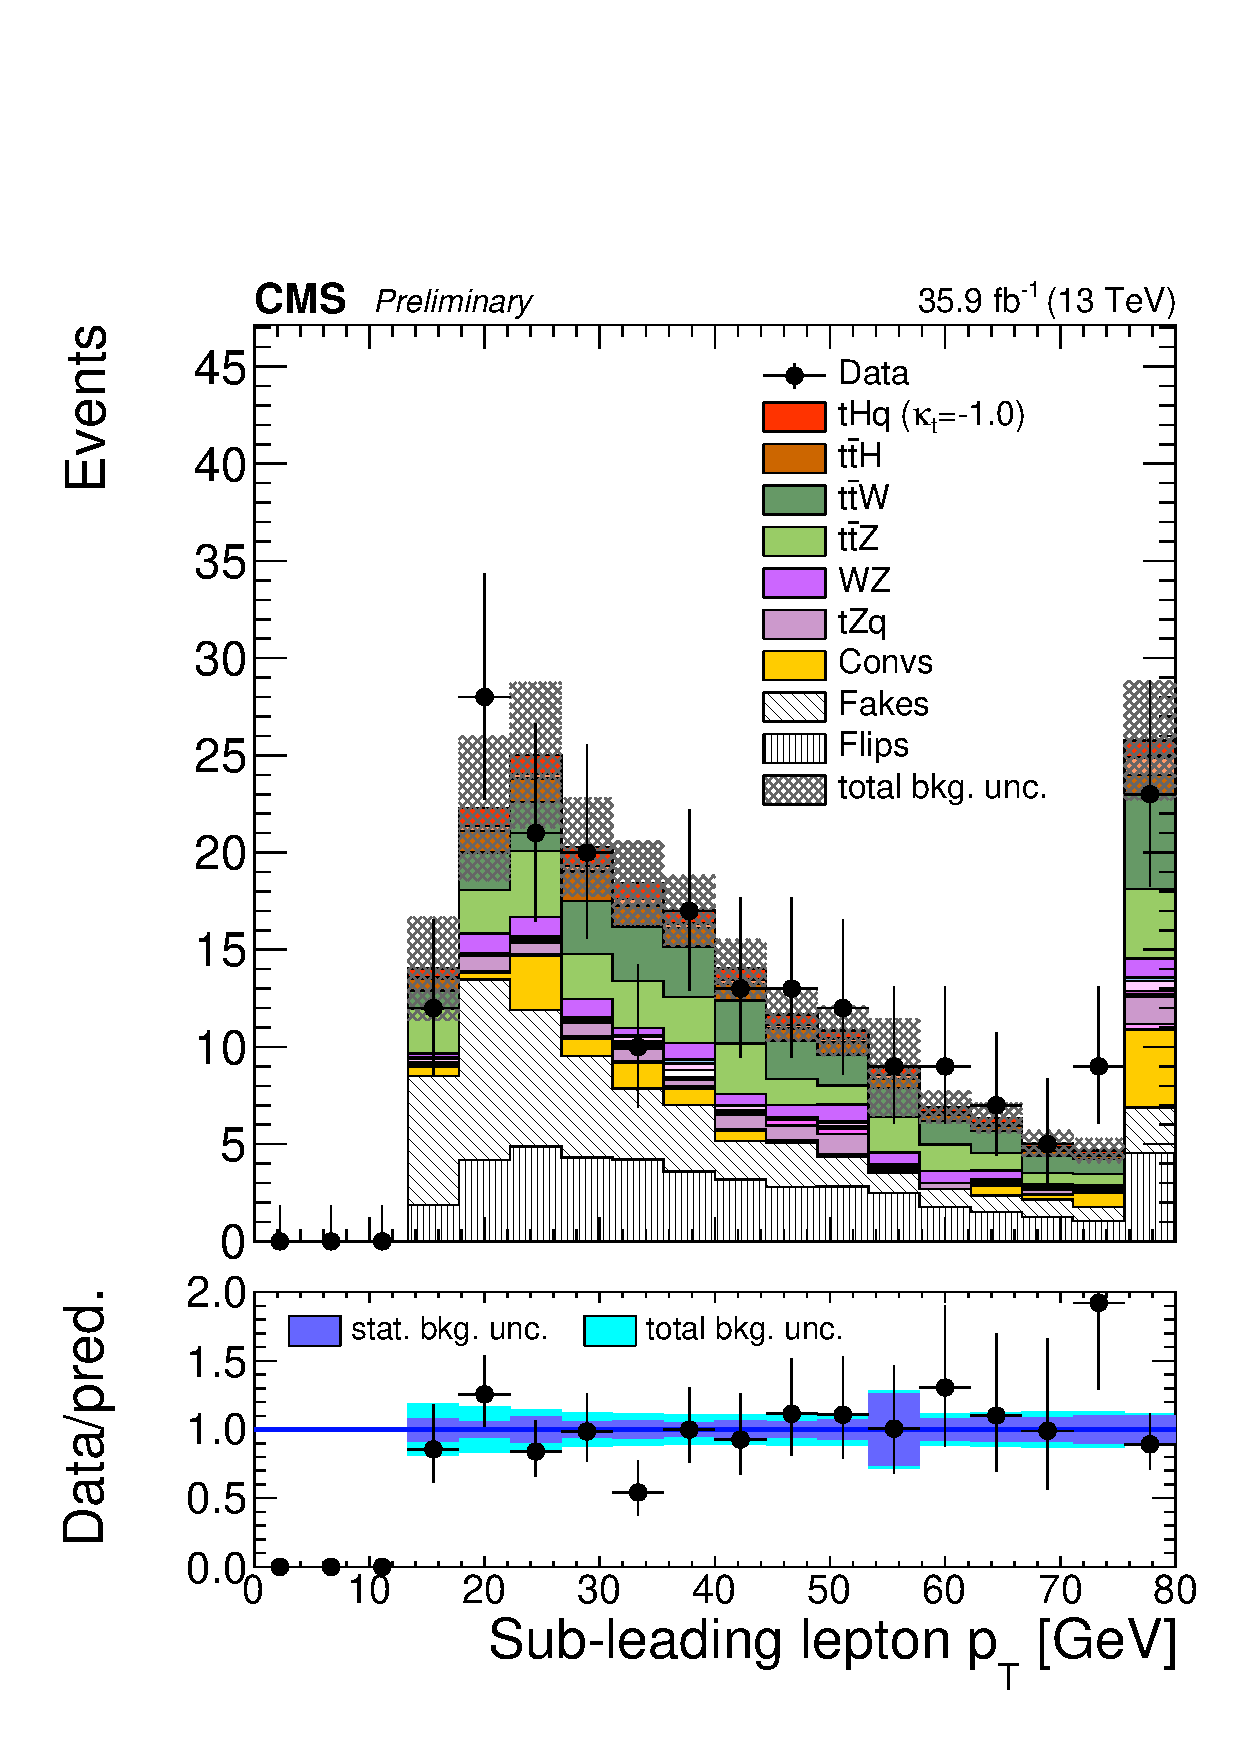
\includegraphics[width=0.22\textwidth]{figures/signalregion_2lss/ee/Lep2Pt.pdf}
  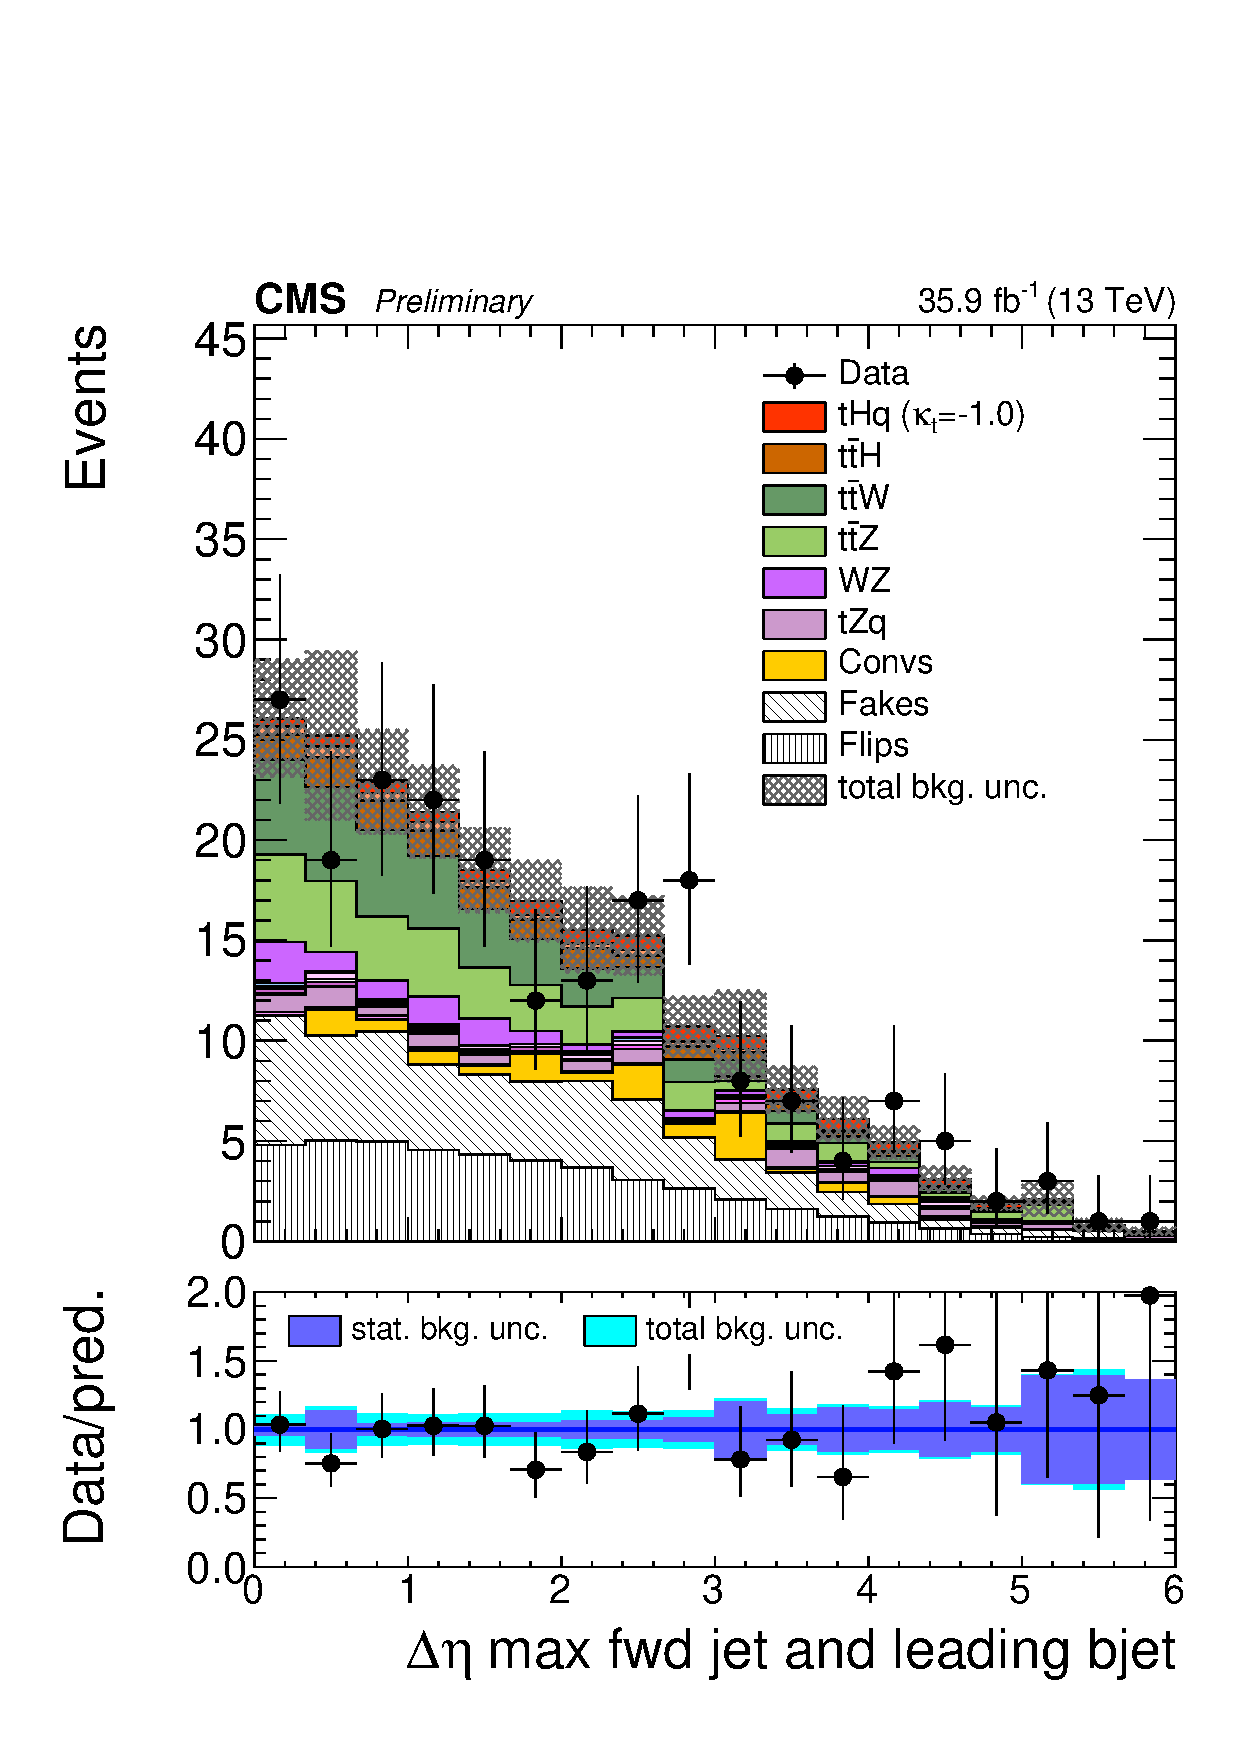
\includegraphics[width=0.22\textwidth]{figures/signalregion_2lss/ee/dEtaFwdJetBJet_40.pdf}
  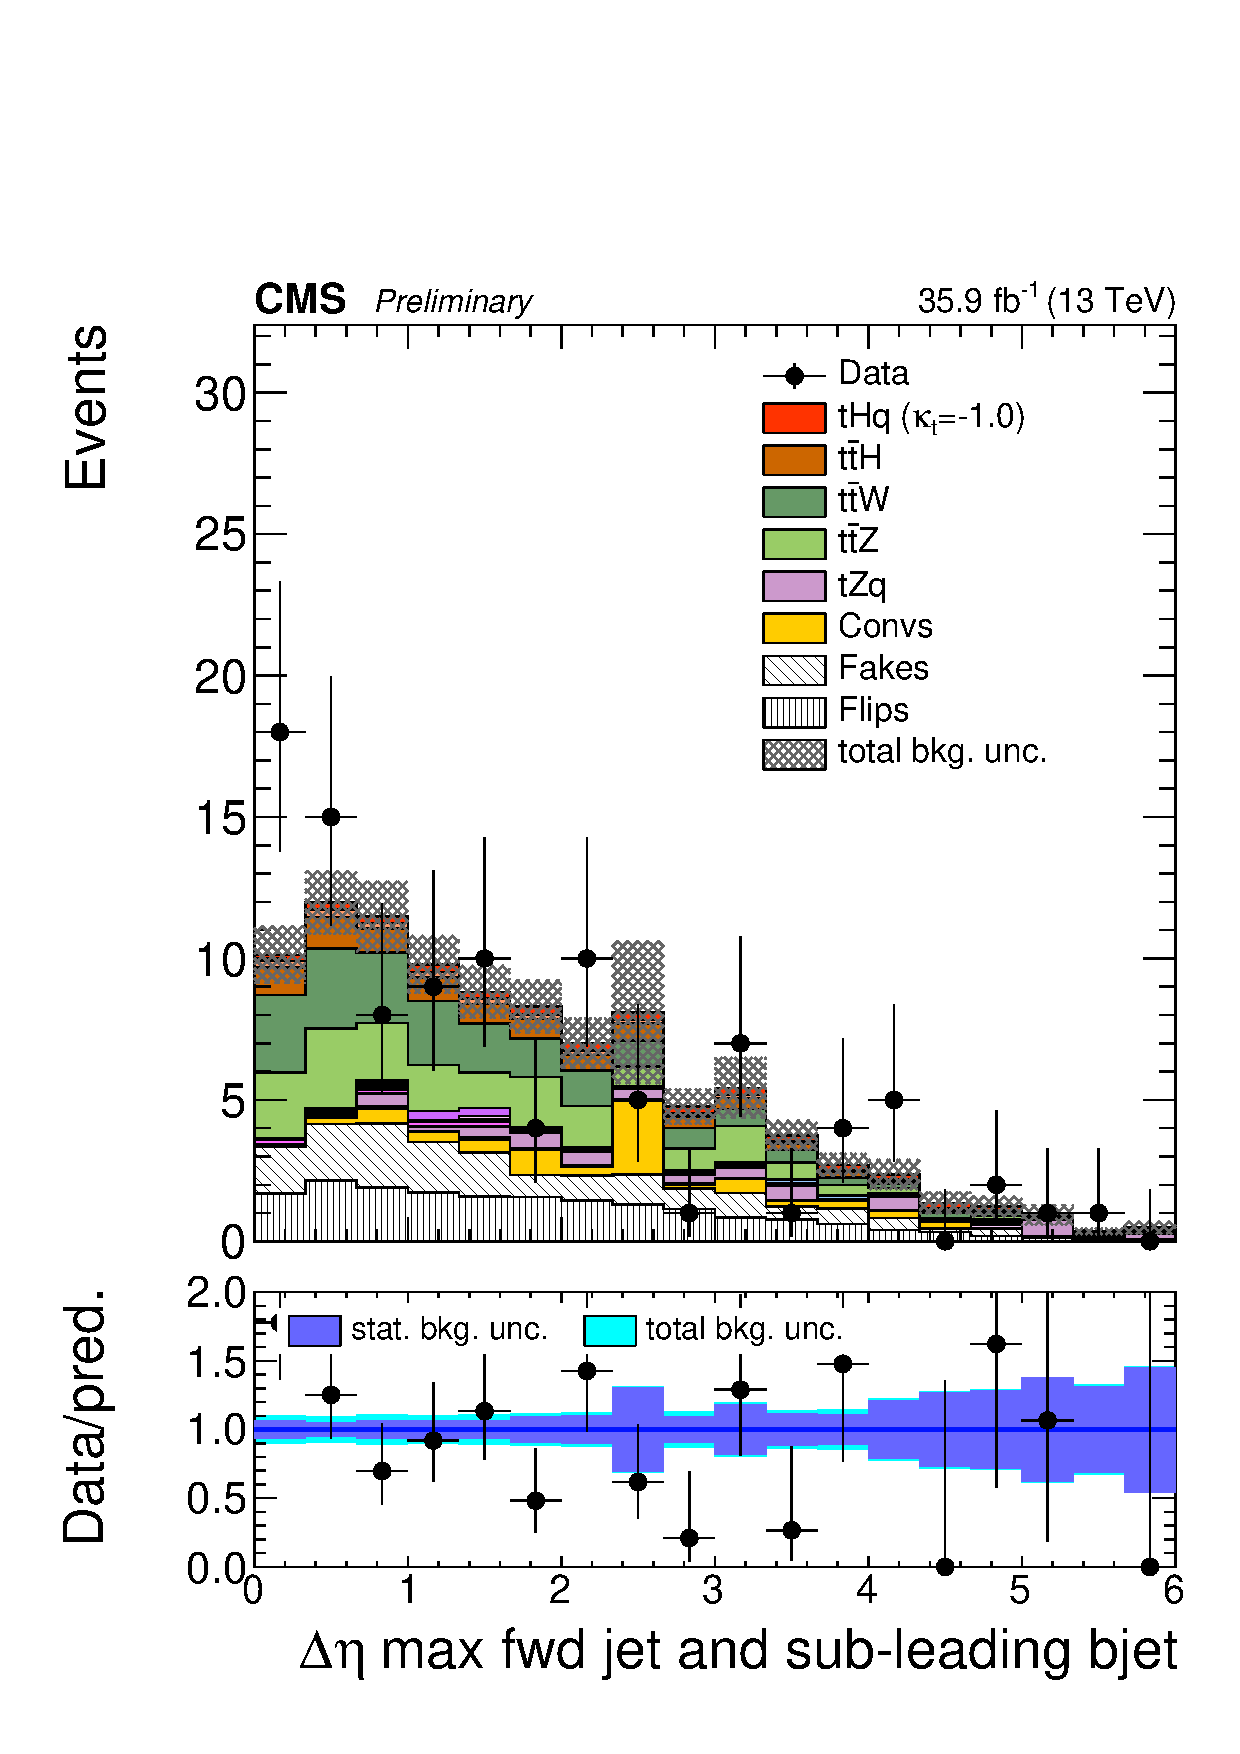
\includegraphics[width=0.22\textwidth]{figures/signalregion_2lss/ee/dEtaFwdJet2BJet_40.pdf}
  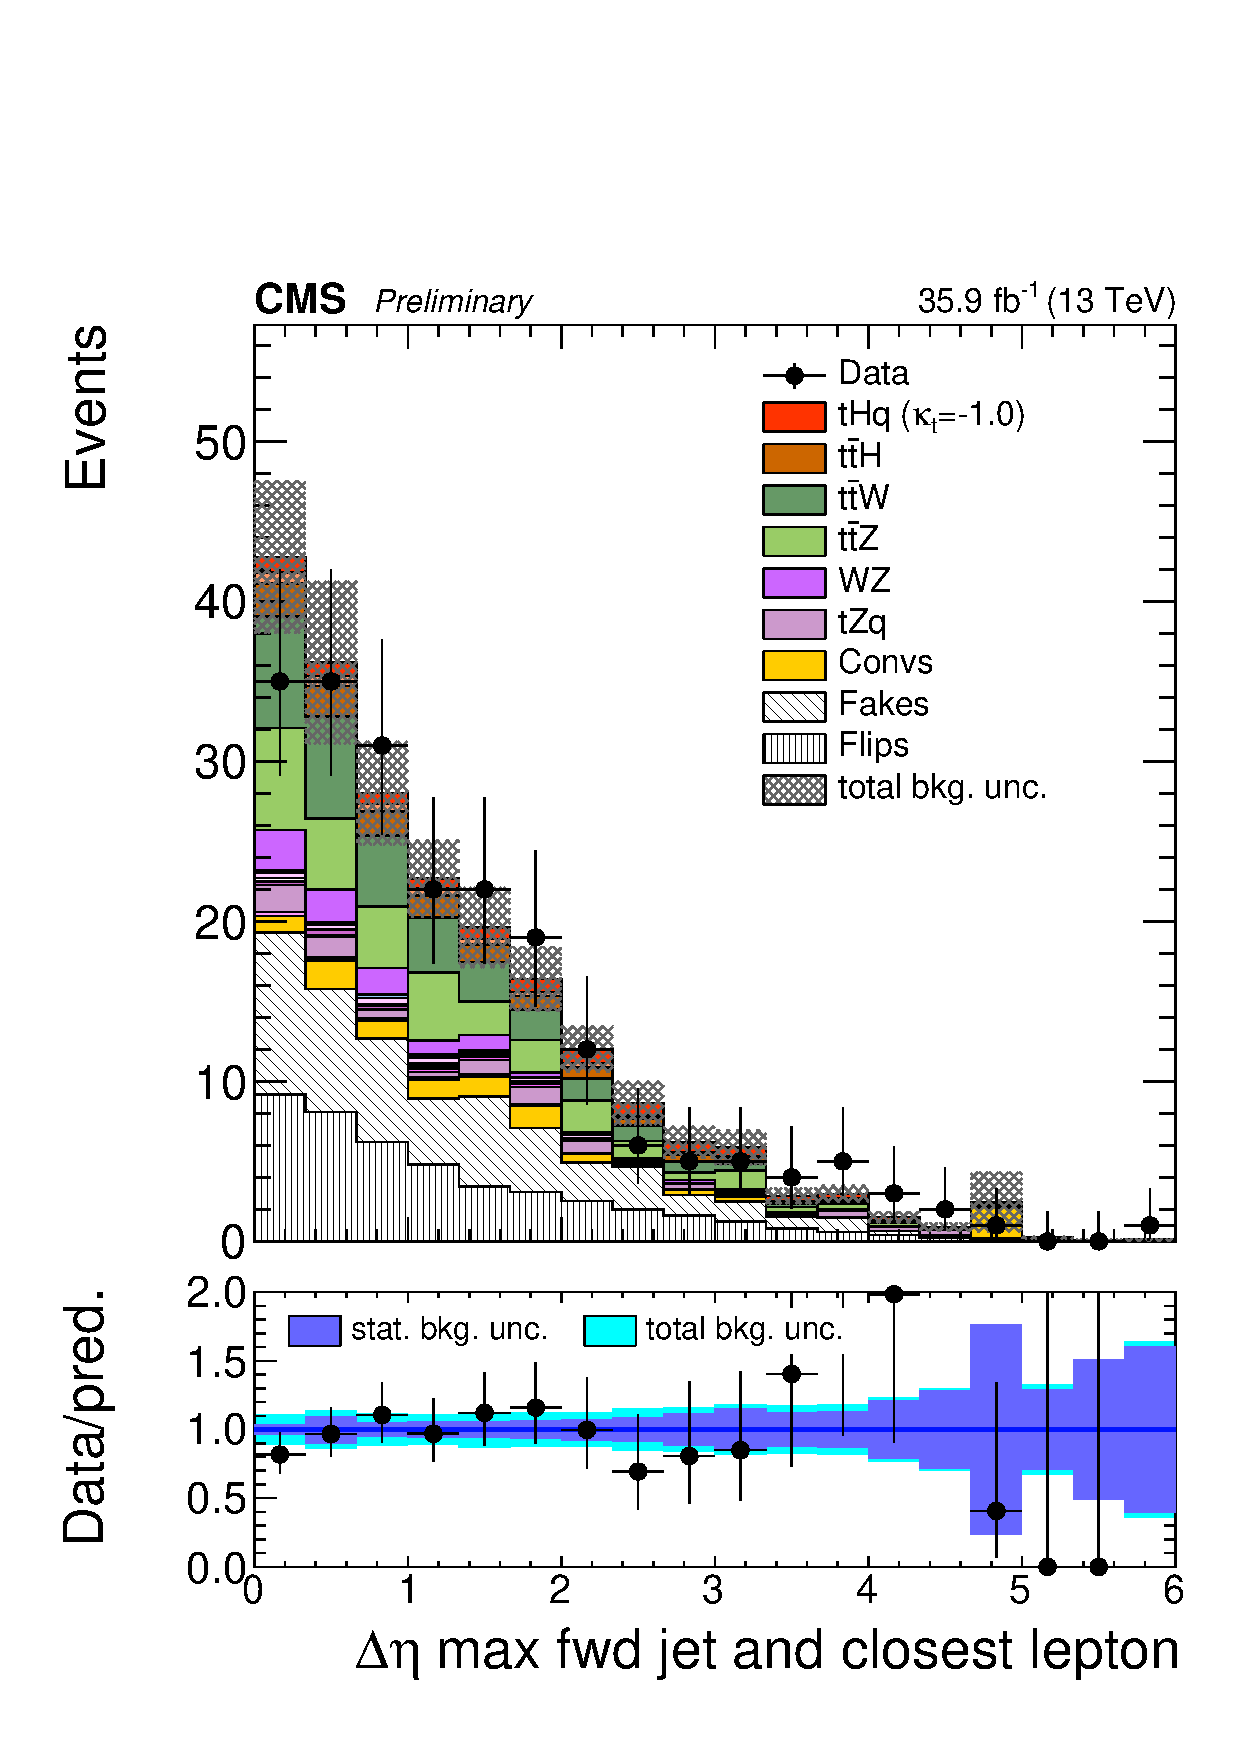
\includegraphics[width=0.22\textwidth]{figures/signalregion_2lss/ee/dEtaFwdJetClosestLep_40.pdf} \\
  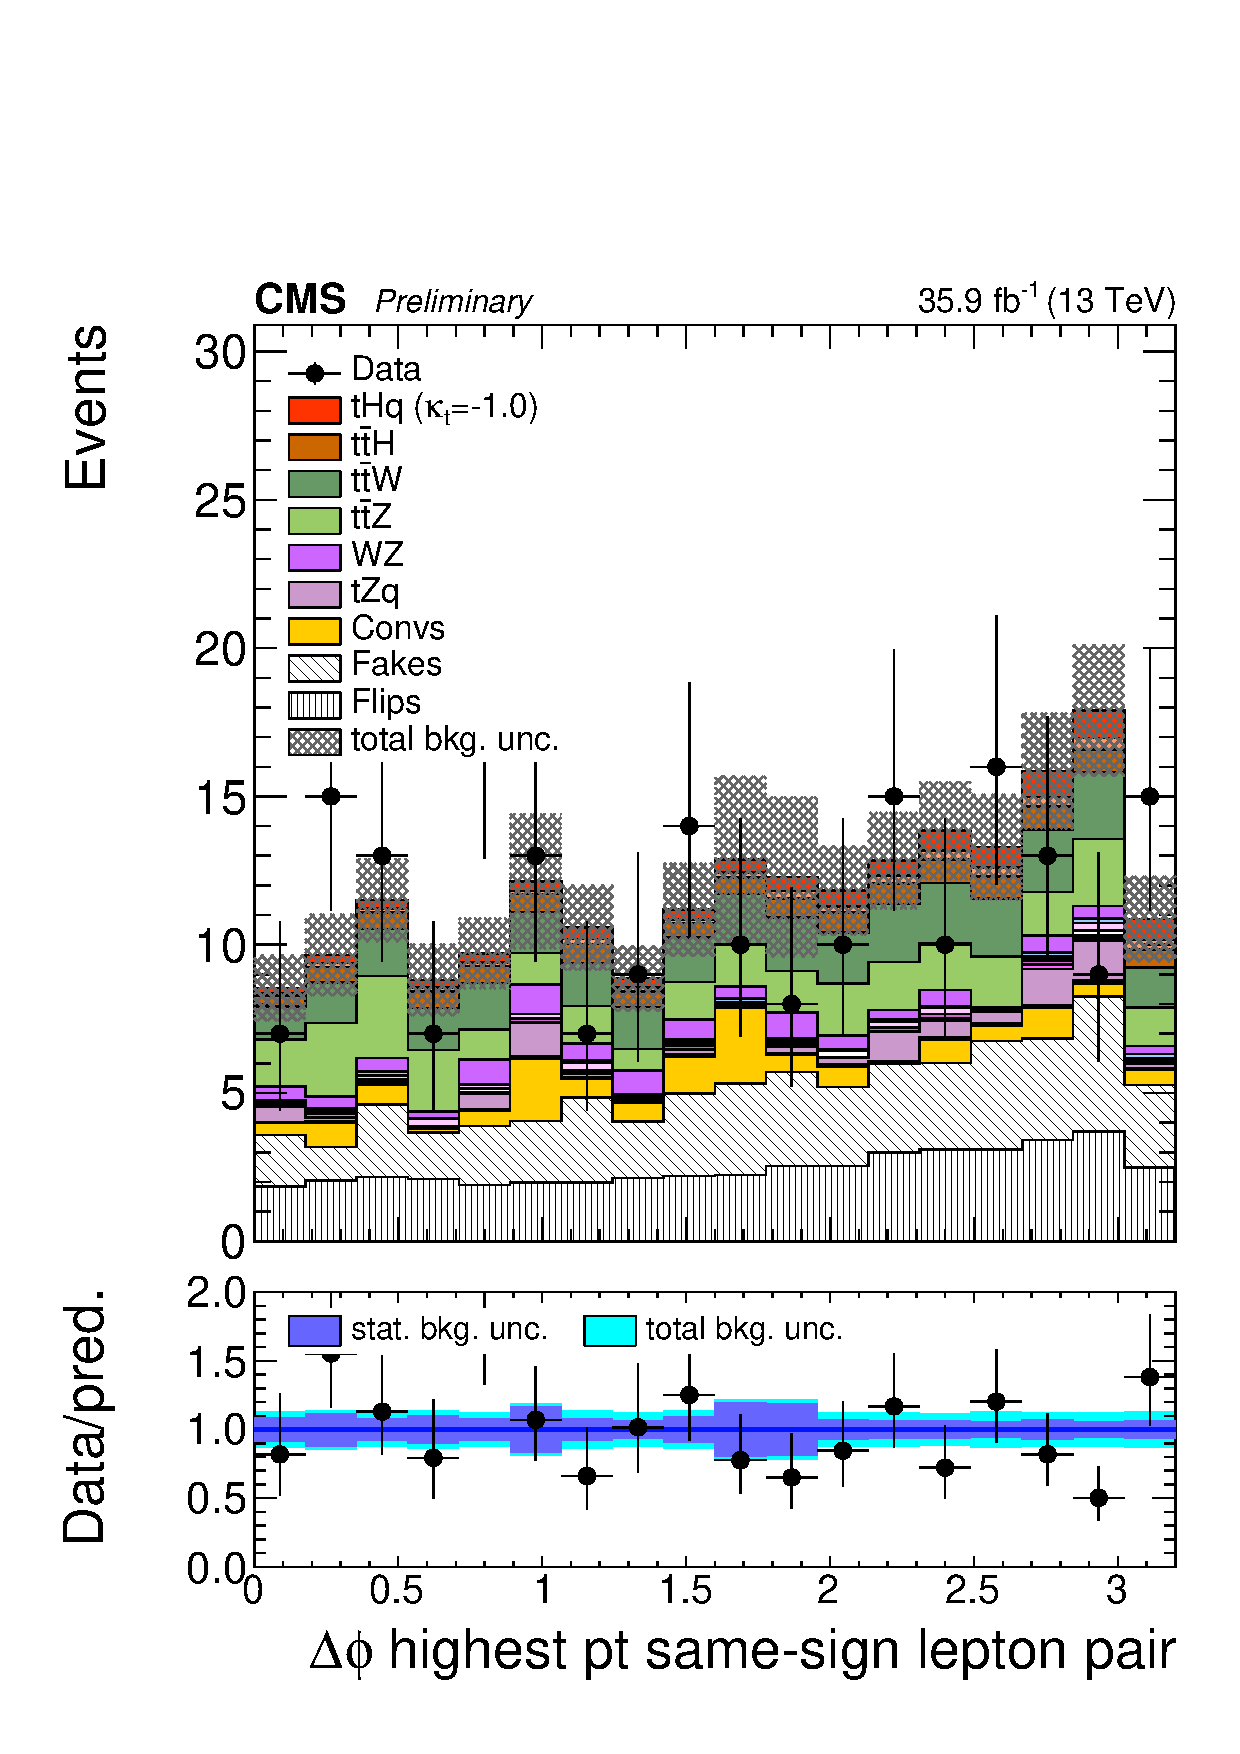
\includegraphics[width=0.22\textwidth]{figures/signalregion_2lss/ee/dPhiHighestPtSSPair.pdf}
  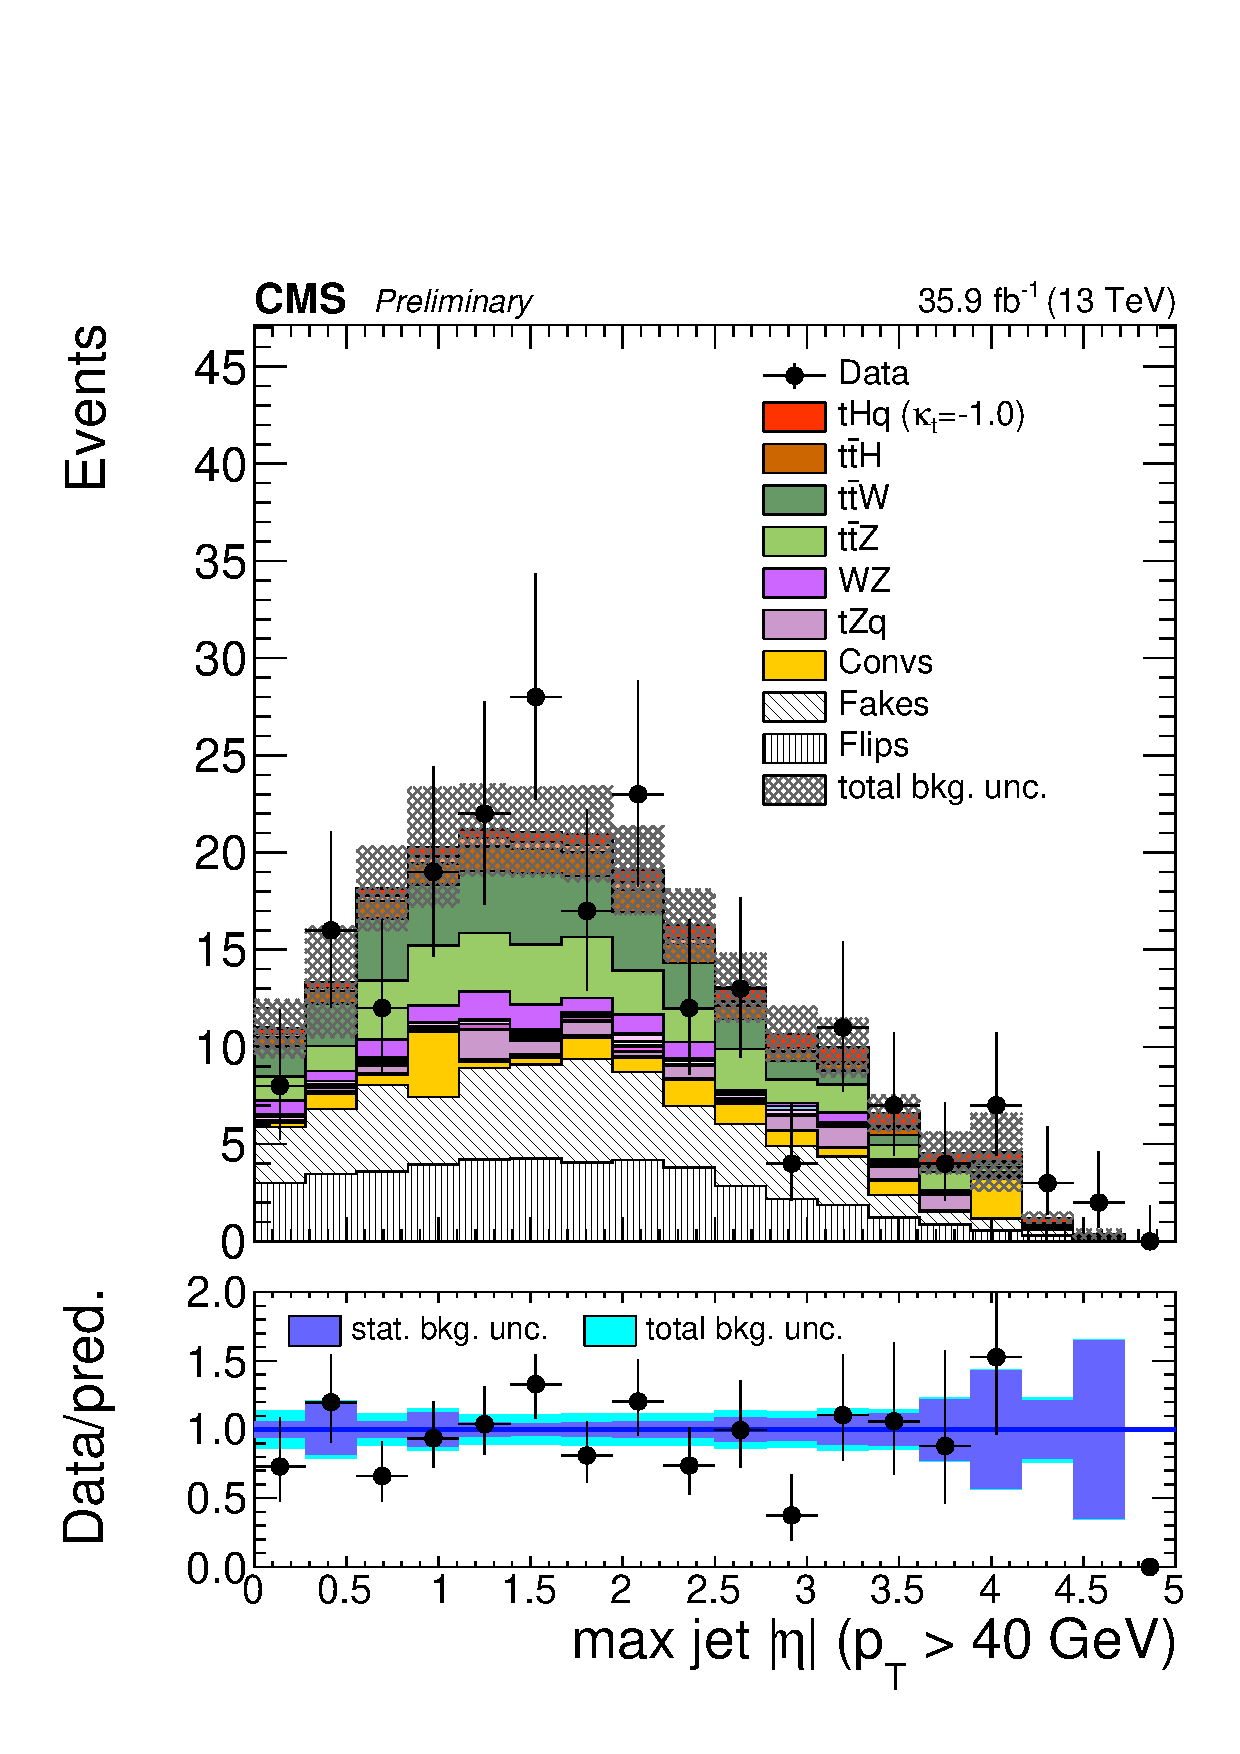
\includegraphics[width=0.22\textwidth]{figures/signalregion_2lss/ee/maxEtaJet25_40.pdf}
  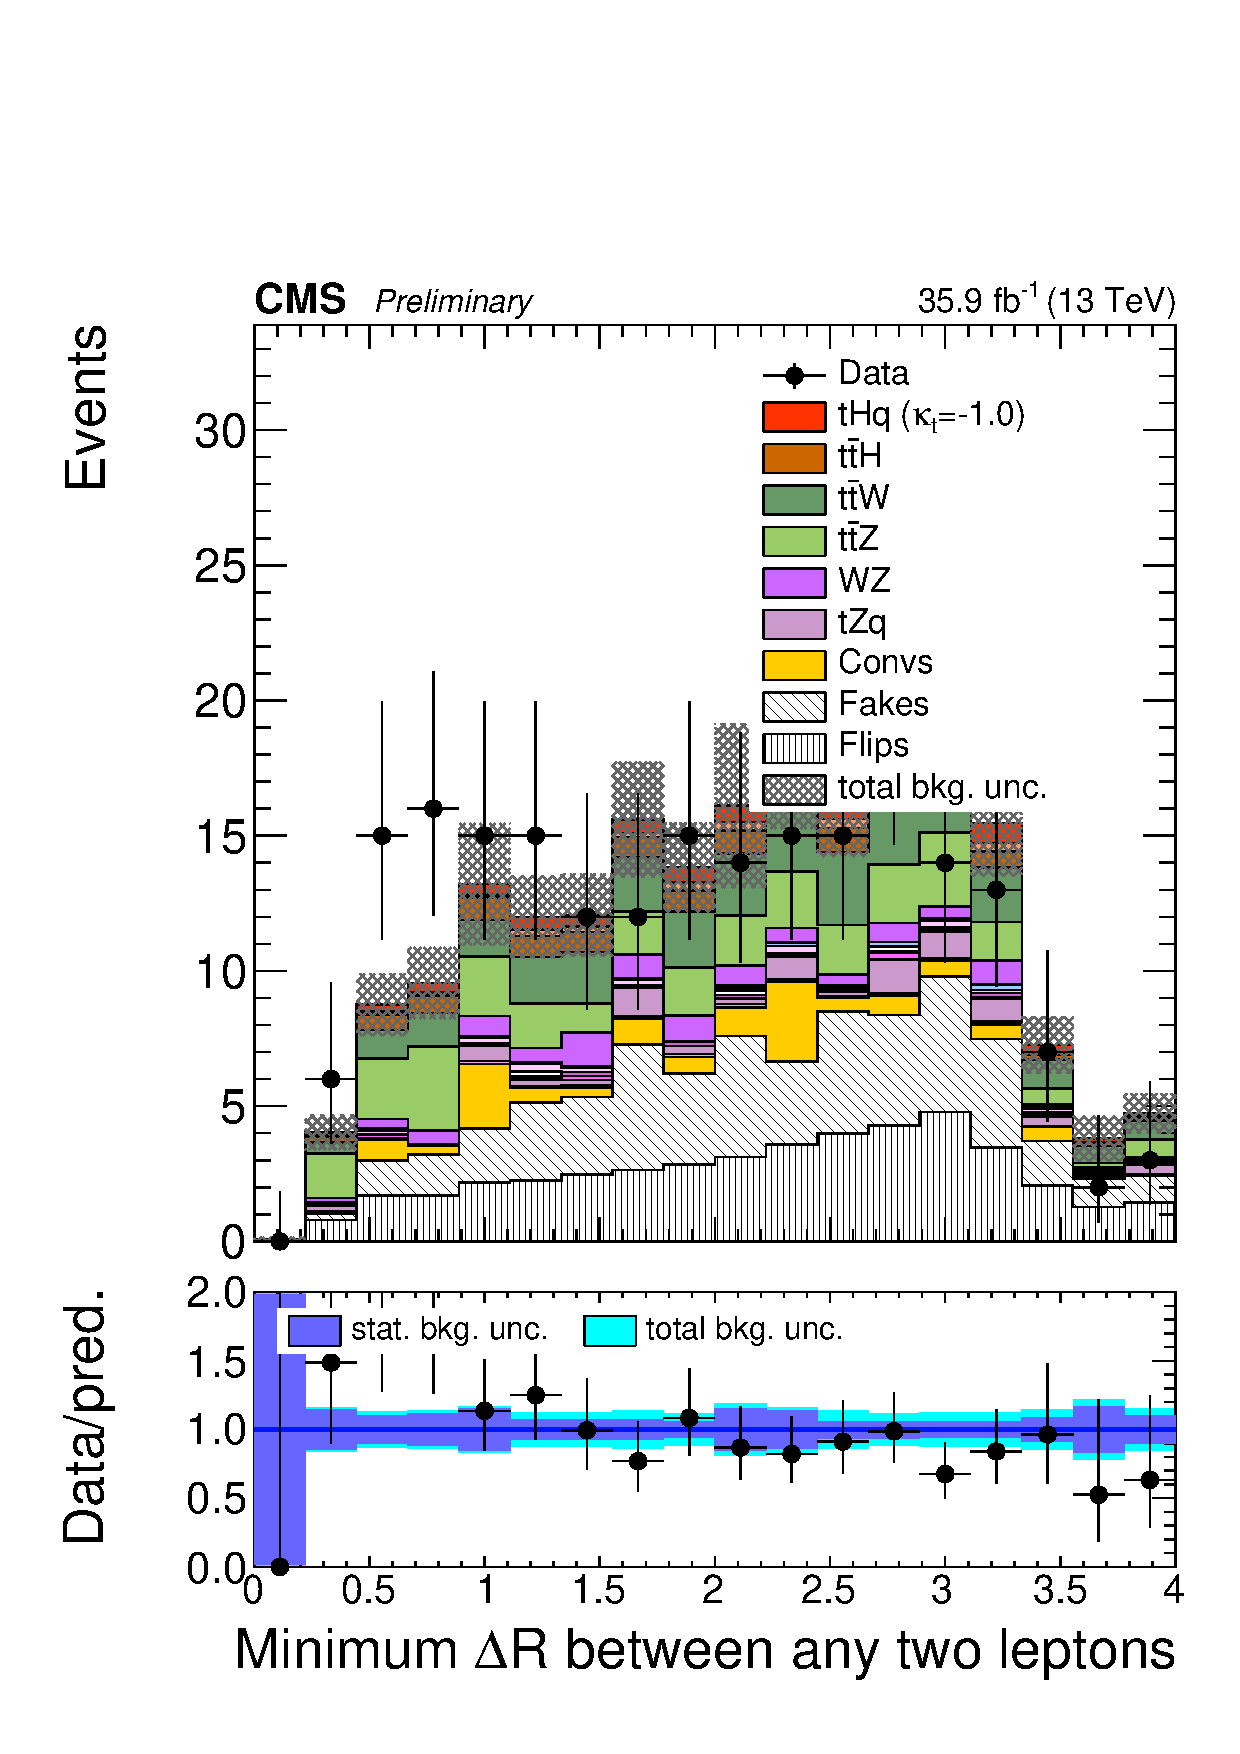
\includegraphics[width=0.22\textwidth]{figures/signalregion_2lss/ee/minDRll.pdf} 
  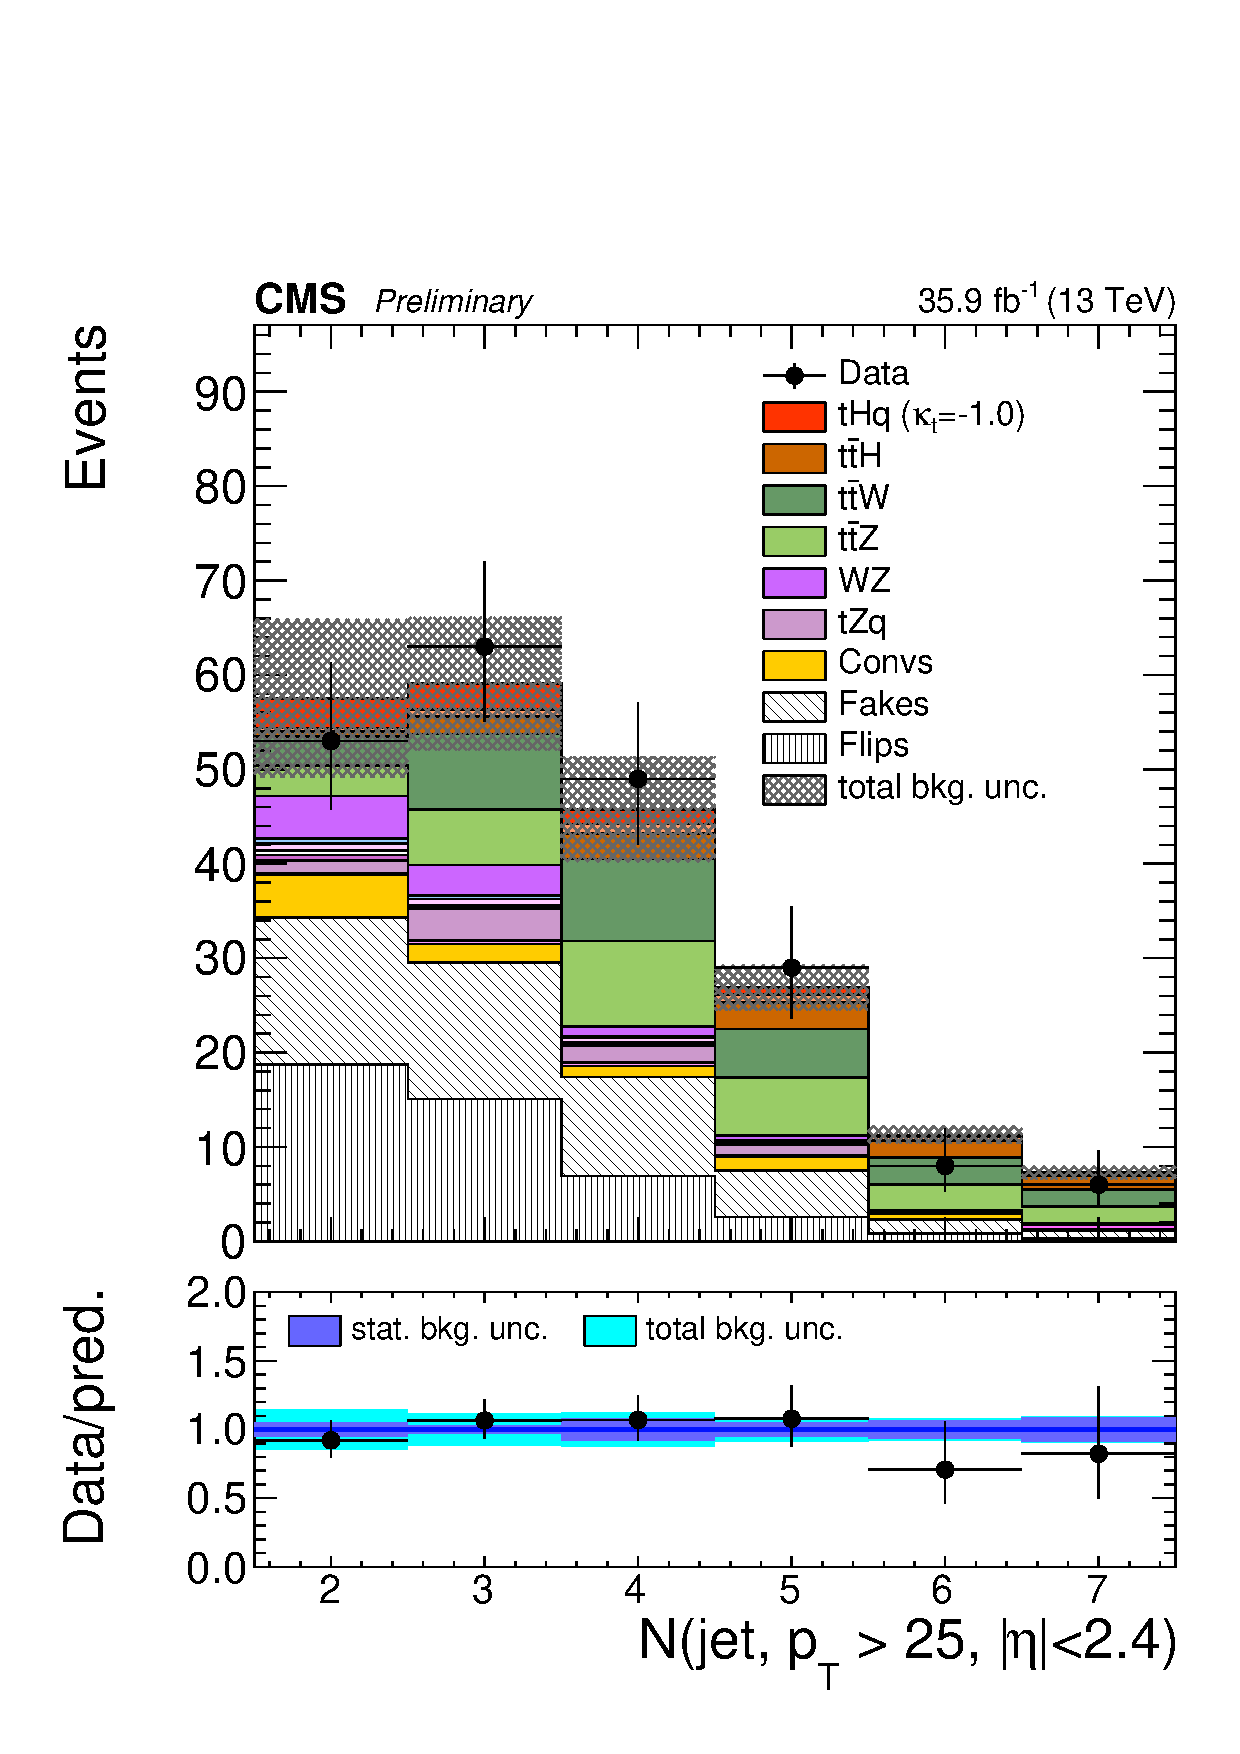
\includegraphics[width=0.22\textwidth]{figures/signalregion_2lss/ee/nJet25.pdf} \\
  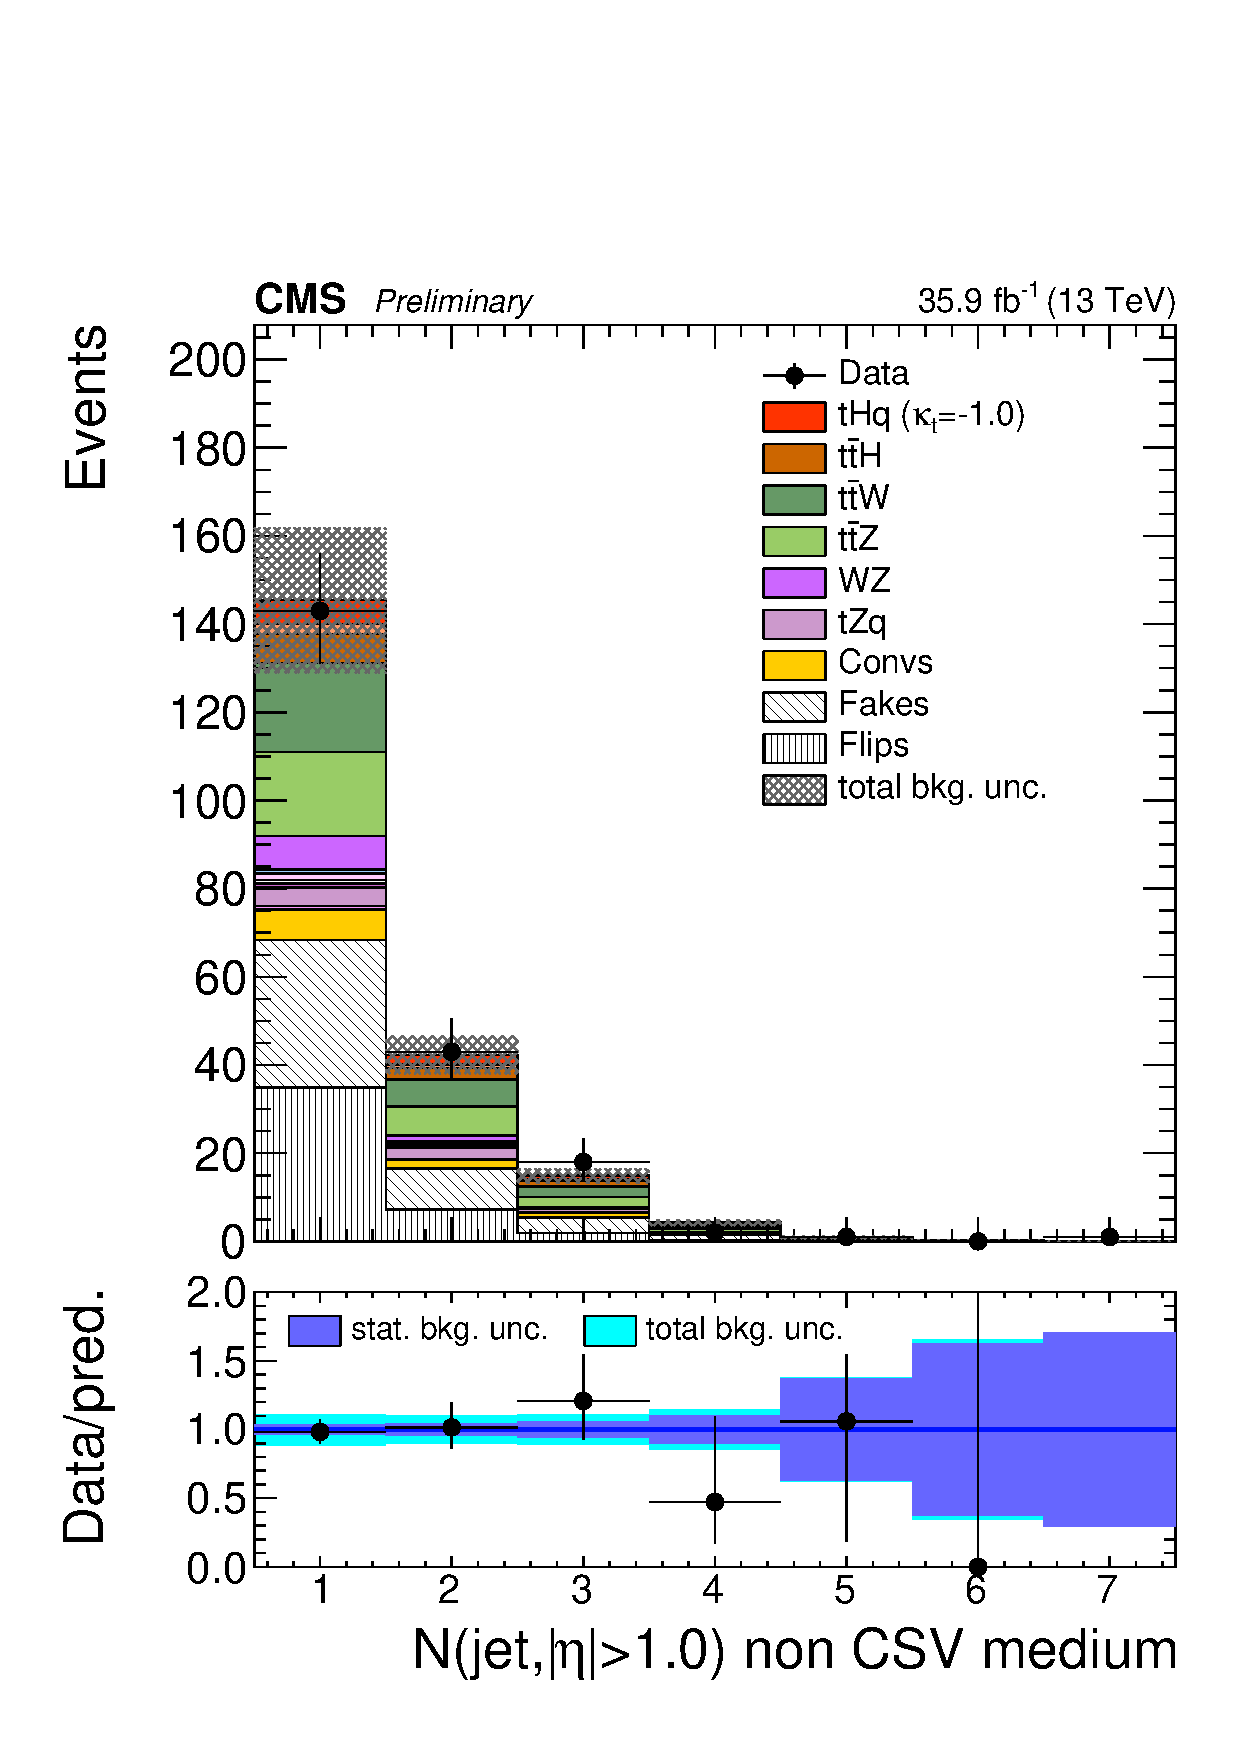
\includegraphics[width=0.22\textwidth]{figures/signalregion_2lss/ee/nJetEta1_40.pdf}
  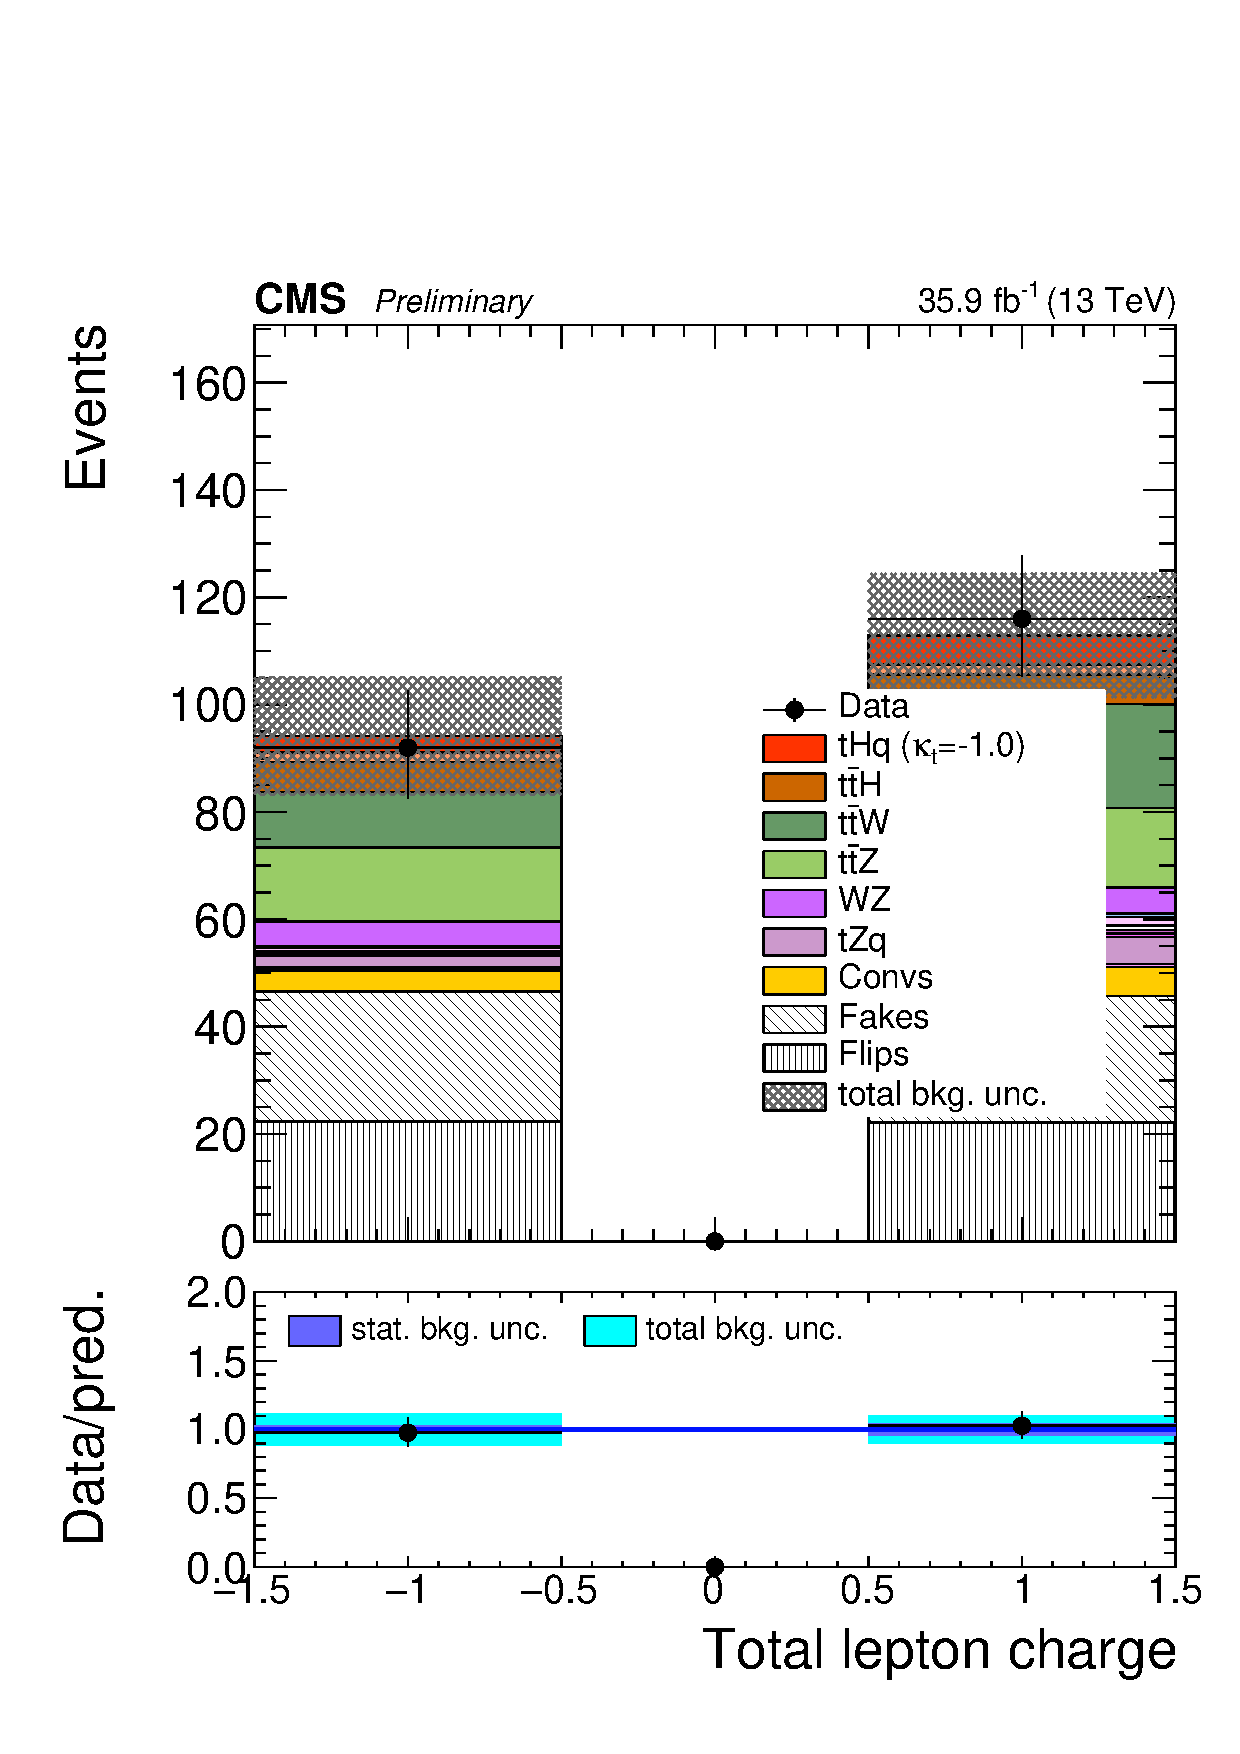
\includegraphics[width=0.22\textwidth]{figures/signalregion_2lss/ee/totCharge.pdf}
\caption{Distributions of input variables to the BDT for signal discrimination, in $\Pe^{\pm}\Pe^{\pm}$ channel, normalized to their cross section and to 35.9\fbinv.}
\label{fig:input_vars_2lss_xsec_ee}
\end{figure}

